% !TeX spellcheck = en-US
% !TeX encoding = utf8
% !TeX program = lualatex
% !BIB program = biber
% -*- coding:utf-8 mod:LaTeX -*-


% vv  scroll down to line 200 for content  vv


\let\ifdeutsch\iffalse
\let\ifenglisch\iftrue
% EN: This file is loaded before the \documentclass command in the main document

% EN: The following package allows \\ at the title page
%     For more information see https://github.com/latextemplates/scientific-thesis-cover/issues/4
\RequirePackage{kvoptions-patch}

\ifenglisch
  \PassOptionsToClass{numbers=noenddot}{scrbook}
\else
  %()Aus scrguide.pdf - der Dokumentation von KOMA-Script)
  %Nach DUDEN steht in Gliederungen, in denen ausschließlich arabische Ziffern für die Nummerierung
  %verwendet werden, am Ende der Gliederungsnummern kein abschließender Punkt
  %(siehe [DUD96, R3]). Wird hingegen innerhalb der Gliederung auch mit römischen Zahlen
  %oder Groß- oder Kleinbuchstaben gearbeitet, so steht am Ende aller Gliederungsnummern ein
  %abschließender Punkt (siehe [DUD96, R4])
  \PassOptionsToClass{numbers=autoendperiod}{scrbook}
\fi

% Warns about outdated packages and missing caption declarations
% See https://www.ctan.org/pkg/nag
\RequirePackage[l2tabu, orthodox]{nag}

%DE: Neue deutsche Trennmuster
%    Siehe http://www.ctan.org/pkg/dehyph-exptl und http://projekte.dante.de/Trennmuster/WebHome
%    Nur für pdflatex, nicht für lualatex
\RequirePackage{ifluatex}
\ifluatex
  % do not load anything
\else
  \ifdeutsch
    \RequirePackage[ngerman=ngerman-x-latest]{hyphsubst}
  \fi
\fi

\documentclass[
  % fontsize=11pt is the standard
  a4paper,  % Standard format - only KOMAScript uses paper=a4 - https://tex.stackexchange.com/a/61044/9075
  twoside,  % we are optimizing for both screen and two-side printing. So the page numbers will jump, but the content is configured to stay in the middle (by using the geometry package)
  bibliography=totoc,
  %               idxtotoc,   %Index ins Inhaltsverzeichnis
  %               liststotoc, %List of X ins Inhaltsverzeichnis, mit liststotocnumbered werden die Abbildungsverzeichnisse nummeriert
  headsepline,
  cleardoublepage=empty,
  parskip=half,
  %               draft    % um zu sehen, wo noch nachgebessert werden muss - wichtig, da Bindungskorrektur mit drin
  draft=false
]{scrbook}

% !TeX encoding = utf8
% -*- coding:utf-8 mod:LaTeX -*-

% EN: This file includes basic packages and sets options. The order of package
%     loading is important
% DE: In dieser Datei werden zuerst die benoetigten Pakete eingebunden und
%     danach diverse Optionen gesetzt. Achtung Reihenfolge ist entscheidend!


%%%
% EN: Styleguide:
% - English comments are prefixed with "EN", German comments are prefixed with "DE"
% - Prefixed headings define the language for the subsequent paragraphs
% - It is tried to organize packages in blocks. One block starts with %%%, then
%   % <heading>, then the options and more text. % followed by %%% end a block.
%
% DE: Styleguide:
%
% Ein sehr kleiner Styleguide. Packages werden in Blöcken organisiert.
% Ein Block beginnt mit drei % in einer Zeile, dann % <Blocküberschrift>, dann
% eine Liste der möglichen Optionen und deren Einstellungen, Gründe und Kommentare
% eine % Zeile in der sonst nichts steht und dann wieder %%% in einer Zeile.
%
% Zwischen zwei Blöcken sind 2 Leerzeilen!
% Zu jedem Paket werden soviele Optionen wie möglich/nötig angegeben
%
%%%


%%%
% EN: Enable copy and paste of text from the PDF
%     Only required for pdflatex. It "just works" in the case of lualatex.
%     mmap enables mathematical symbols, but does not work with the newtx font set
%     See: https://tex.stackexchange.com/a/64457/9075
%     Other solutions outlined at http://goemonx.blogspot.de/2012/01/pdflatex-ligaturen-und-copynpaste.html and http://tex.stackexchange.com/questions/4397/make-ligatures-in-linux-libertine-copyable-and-searchable
%     Trouble shooting outlined at https://tex.stackexchange.com/a/100618/9075
\ifluatex
\else
  \usepackage{cmap}
\fi
%%%


%%%
% EN: File encoding
% DE: Codierung
%     Wir sind im 21 Jahrhundert, utf-8 löst so viele Probleme.
%
% Mit UTF-8 funktionieren folgende Pakete nicht mehr. Bitte beachten!
%   * fancyvrb mit §
%   * easylist -> http://www.ctan.org/tex-archive/macros/latex/contrib/easylist/
\ifluatex
  % EN: See https://tex.stackexchange.com/a/158517/9075
  %     Not required, because of usage of fontspec package
  %\usepackage[utf8]{luainputenc}
\else
  \usepackage[utf8]{inputenc}
\fi
%
%%%

%%%
% DE: Parallelbetrieb tex4ht und pdflatex
\makeatletter
\@ifpackageloaded{tex4ht}{
  \def\iftex4ht{\iftrue}
}{
  \def\iftex4ht{\iffalse}
}
\makeatother
%%%


%%%
% EN: Defintion of colors
% DE: Farbdefinitionen
\usepackage[hyperref,dvipsnames]{xcolor}
%

%%%
% EN: Required for custom acronyms/glossaries style.
%     Left aligned Columns in tables with fixed width.
%     See http://tex.stackexchange.com/questions/91566/syntax-similar-to-centering-for-right-and-left
\usepackage{ragged2e}
%%%

%%%
% EN: Abbreviations
% DE: Abkürzungsverzeichnis
%
% DE: Wichtig, ansonsten erscheint "No room for a new \write"
\usepackage{scrwfile}
% DE: siehe http://www.dickimaw-books.com/cgi-bin/faq.cgi?action=view&categorylabel=glossaries#glsnewwriteexceeded
\usepackage[acronym,indexonlyfirst,nomain]{glossaries}
\ifdeutsch
  \renewcommand*{\acronymname}{Abkürzungsverzeichnis}
\else
  \renewcommand*{\acronymname}{List of Abbreviations}
\fi
\renewcommand*{\glsgroupskip}{}
%
% EN: Removed Glossarie as a table as a quick fix to get the template working again
%     See http://tex.stackexchange.com/questions/145579/how-to-print-acronyms-of-glossaries-into-a-table
%
\makenoidxglossaries
%%%


%%%
% EN: Support for language-specific hyphenation
% DE: Neue deutsche Rechtschreibung und Literatur statt "Literature"
%     Die folgende Einstellung ist der Nachfolger von ngerman.sty
\ifdeutsch
  % DE: letzte Sprache ist default, Einbindung von "american" ermöglicht \begin{otherlanguage}{amercian}...\end{otherlanguage} oder \foreignlanguage{american}{Text in American}
  %     Siehe auch http://tex.stackexchange.com/a/50638/9075
  \usepackage[american,ngerman]{babel}
  % Ein "abstract" ist eine "Kurzfassung", keine "Zusammenfassung"
  \addto\captionsngerman{%
    \renewcommand\abstractname{Kurzfassung}%
  }
  \ifluatex
    % EN: conditionally disable ligatures. See https://github.com/latextemplates/scientific-thesis-template/issues/54
    %     for a discussion
    \usepackage[ngerman]{selnolig}
  \fi
\else
  % EN: Set English as language and allow to write hyphenated"=words
  %     `american`, `english` and `USenglish` are synonyms for babel package (according to https://tex.stackexchange.com/questions/12775/babel-english-american-usenglish).
  %      "english" has to go last to set it as default language
  \usepackage[ngerman,english]{babel}
  % EN: Hint by http://tex.stackexchange.com/a/321066/9075 -> enable "= as dashes
  \addto\extrasenglish{\languageshorthands{ngerman}\useshorthands{"}}
  \ifluatex
    % EN: conditionally disable ligatures. See https://github.com/latextemplates/scientific-thesis-template/issues/54
    %     for a discussion
    \usepackage[english]{selnolig}
  \fi
\fi
%
%%%


%%%
% EN: For easy quotations: \enquote{text}
%     This package is very smart when nesting is applied, otherwise textcmds (see below) provides a shorter command
% DE:  Anführungszeichen
%      Zitate in \enquote{...} setzen, dann werden automatisch die richtigen Anführungszeichen verwendet.
\usepackage{csquotes}
%%%


%%%
% EN: For even easier quotations: \qq{text}.
%     Is not smart in the case of nesting, but good enough for the most cases
\usepackage{textcmds}
\ifdeutsch
  % EN: German quotes are different. So do not use the English quotes, but the ones provided by the csquotes package.
  \renewcommand{\qq}[1]{\enquote{#1}}
\fi
%%%


%%%
% EN: extended enumarations
% DE: erweitertes Enumerate
\usepackage{paralist}
%
%%%


%%%
% DE: fancyheadings (nicht nur) fuer koma
\usepackage[automark]{scrlayer-scrpage}
%
%%%


%%%
% EN: Mathematics
% DE: Mathematik
%
% DE: Viele Mathematik-Sachen. Siehe https://texdoc.net/pkg/amsmath
\usepackage{amsmath}
% EN: Options must be passed this way, otherwise it does not work with glossaries
\PassOptionsToPackage{fleqn,leqno}{amsmath}
% DE: fleqn (=Gleichungen linksbündig platzieren) funktioniert nicht direkt. Es muss noch ein Patch gemacht werden:
%\addtolength\mathindent{1em}%work-around ams-math problem with align and 9 -> 10. Does not work with glossaries, No visual changes.
% EN: Fixes bugs in AMS math
\usepackage{mathtools}
%
% EN: For theorems, replacement for amsthm
\usepackage[amsmath,hyperref]{ntheorem}
\theorempreskipamount 2ex plus1ex minus0.5ex
\theorempostskipamount 2ex plus1ex minus0.5ex
\theoremstyle{break}
\newtheorem{definition}{Definition}[section]
%
%%%


%%%
% DE: Intelligentes Leerzeichen um hinter Abkürzungen die richtigen Abstände zu erhalten, auch leere.
%     Siehe commands.tex \gq{}
\usepackage{xspace}
%DE: Macht \xspace und \enquote kompatibel
\makeatletter
\xspaceaddexceptions{\grqq \grq \csq@qclose@i \} }
\makeatother
%
%%%


%%%
% EN: Package for the appendix
% DE: Anhang
\usepackage{appendix}
%[toc,page,title,header]
%
%%%

%%%
% EN: Graphics
% DE: Grafikeinbindungen
%
% EN: The parameter "pdftex" is not required
\usepackage{graphicx}
\graphicspath{{\getgraphicspath}}
\newcommand{\getgraphicspath}{graphics/}
%
%%%


%%%
% EN: Enables inclusion of SVG graphics - 1:1 approach
%    This is NOT the approach of https://ctan.org/pkg/svg-inkscape,
%     which allows text in SVG to be typeset using LaTeX
%     We just include the SVG as is.
\usepackage{epstopdf}
\epstopdfDeclareGraphicsRule{.svg}{pdf}{.pdf}{%
  inkscape -z -D --file=#1 --export-pdf=\OutputFile
}
%
%%%


%%%
% EN: Enables inclusion of SVG graphics - text-rendered-with-LaTeX-approach
%     This is the approach of https://ctan.org/pkg/svg-inkscape,
\newcommand{\executeiffilenewer}[3]{%
  \IfFileExists{#2}
  {
    %\message{file #2 exists}
    \ifnum\pdfstrcmp{\pdffilemoddate{#1}}%
      {\pdffilemoddate{#2}}>0%
      {\immediate\write18{#3}}
    \else
      {%\message{file up to date #2}
      }
    \fi%
  }{
    %\message{file #2 doesn't exist}
    %\message{argument: #3}
    %\immediate\write18{echo "test" > xoutput.txt}
    \immediate\write18{#3}
  }
}
\newcommand{\includesvg}[1]{%
  \executeiffilenewer{#1.svg}{#1.pdf}%
  {
    inkscape -z -D --file=\getgraphicspath#1.svg %
    --export-pdf=\getgraphicspath#1.pdf --export-latex}%
  \input{\getgraphicspath#1.pdf_tex}%
}


%%%
% EN: Enable typesetting values with SI units.
\ifdeutsch
  \usepackage[mode=text,group-four-digits]{siunitx}
  \sisetup{locale=DE}
\else
  \usepackage[mode=text,group-four-digits,group-separator={,}]{siunitx}
  \sisetup{locale=US}
\fi
%%%

%%%
% EN: Extensions for tables
% DE: Tabellenerweiterungen
\usepackage{array} %increases tex's buffer size and enables ``>'' in tablespecs
\usepackage{longtable}
\usepackage{dcolumn} %Aligning numbers by decimal points in table columns
\ifdeutsch
  \newcolumntype{d}[1]{D{.}{,}{#1}}
\else
  \newcolumntype{d}[1]{D{.}{.}{#1}}
\fi
\setlength{\extrarowheight}{1pt}
%%%

%%%
% Eine Zelle, die sich über mehrere Zeilen erstreckt.
% Siehe Beispieltabelle in Kapitel 2
\usepackage{multirow}
%
%%%

%%%
%Fuer Tabellen mit Variablen Spaltenbreiten
%\usepackage{tabularx}
%\usepackage{tabulary}
%
%%%


%%%
% EN: Links behave as they should. Enables "\url{...}" for URL typesettings.
%     Allow URL breaks also at a hyphen, even though it might be confusing: Is the "-" part of the address or just a hyphen?
%     See https://tex.stackexchange.com/a/3034/9075.
% DE: Links verhalten sich so, wie sie sollen
%     Zeilenumbrüche bei URLs auch bei Bindestrichen erlauben, auch wenn es verwirrend sein könnte: Gehört der Bindestrich zur URL oder ist es ein Trennstrich?
%     Siehe https://tex.stackexchange.com/a/3034/9075.
\usepackage[hyphens]{url}
%
%  EN: When activated, use text font as url font, not the monospaced one.
%      For all options see https://tex.stackexchange.com/a/261435/9075.
% \urlstyle{same}
%
% EN: Hint by http://tex.stackexchange.com/a/10419/9075.
\makeatletter
\g@addto@macro{\UrlBreaks}{\UrlOrds}
\makeatother
%
%%%


%%%
% Index über Begriffe, Abkürzungen
%\usepackage{makeidx} makeidx ist out -> http://xindy.sf.net verwenden
%
%%%

%%%
%lustiger Hack fuer das Abkuerzungsverzeichnis
%nach latex durchlauf folgendes ausfuehren
%makeindex ausarbeitung.nlo -s nomencl.ist -o ausarbeitung.nls
%danach nochmal latex
%\usepackage{nomencl}
%    \let\abk\nomenclature %Deutsche Ueberschrift setzen
%          \renewcommand{\nomname}{List of Abbreviations}
%        %Punkte zw. Abkuerzung und Erklaerung
%          \setlength{\nomlabelwidth}{.2\hsize}
%          \renewcommand{\nomlabel}[1]{#1 \dotfill}
%        %Zeilenabstaende verkleinern
%          \setlength{\nomitemsep}{-\parsep}
%    \makenomenclature
%
%%%

%%%
% EN: Logic for TeX - enables if-then-else in commands
% DE: Logik für TeX
%     FÜr if-then-else @ commands.tex
\usepackage{ifthen}
%
%%%


%%%
% EN: Code Listings
% DE: Listings
\usepackage{listings}
\lstset{language=XML,
  showstringspaces=false,
  extendedchars=true,
  basicstyle=\footnotesize\ttfamily,
  commentstyle=\slshape,
  % DE: Original: \rmfamily, damit werden die Strings im Quellcode hervorgehoben. Zusaetzlich evtl.: \scshape oder \rmfamily durch \ttfamily ersetzen. Dann sieht's aus, wie bei fancyvrb
  stringstyle=\ttfamily,
  breaklines=true,
  breakatwhitespace=true,
  % EN: alternative: fixed
  columns=flexible,
  numbers=left,
  numberstyle=\tiny,
  basewidth=.5em,
  xleftmargin=.5cm,
  % aboveskip=0mm, %DE: deaktivieren, falls man lstlistings direkt als floating object benutzt (\begin{lstlisting}[float,...])
  % belowskip=0mm, %DE: deaktivieren, falls man lstlistings direkt als floating object benutzt (\begin{lstlisting}[float,...])
  captionpos=b
}

\ifluatex
\else
  % EN: Enable UTF-8 support - see https://tex.stackexchange.com/q/419327/9075
  \usepackage{listingsutf8}
  \lstset{inputencoding=utf8/latin1}
\fi

\ifdeutsch
  \renewcommand{\lstlistlistingname}{Verzeichnis der Listings}
\fi
%
%%%


%%%
% EN: Alternative to listings could be fancyvrb. Can be used together.
% DE: Alternative zu Listings ist fancyvrb. Kann auch beides gleichzeitig benutzt werden.
\usepackage{fancyvrb}
%
%EN: Font size for the normal text
%DE: Groesse fuer den Fliesstext. Falls deaktiviert: \normalsize
%\fvset{fontsize=\small}
%
%DE: Somit kann im Text ganz einfach §verbatim§ text gesetzt werden.
%    Disabled, because UTF-8 does not work any more and lualatex causes issues
%\DefineShortVerb{\§}
%
%EN: Shrink font size of listings
\RecustomVerbatimEnvironment{Verbatim}{Verbatim}{fontsize=\footnotesize}
\RecustomVerbatimCommand{\VerbatimInput}{VerbatimInput}{fontsize=\footnotesize}
%
%EN: Hack for fancyvrb based on http://newsgroups.derkeiler.com/Archive/Comp/comp.text.tex/2008-12/msg00075.html
%EN: Change of the solution: \Vref somehow collidated with cleveref/varioref as the output of \Vref{} was "Abschnitt 4.3 auf Seite 85"; therefore changed to \myVref -- so completely removed
\newcommand{\Vlabel}[1]{\label[line]{#1}\hypertarget{#1}{}}
\newcommand{\lref}[1]{\hyperlink{#1}{\FancyVerbLineautorefname~\ref*{#1}}}
%
%%%


%%%
% EN: Tunings of captions for floats, listings, ...
% DE: Bildunterschriften bei floats genauso formatieren wie bei Listings
%     Anpassung wird unten bei den newfloat-Deklarationen vorgenommen
%     https://www.ctan.org/pkg/caption2 is superseeded by this package.
\usepackage{caption}
%
%%%


%%%
% EN: Provides rotating figures, where the PDF page is also turned
% DE: Ermoeglicht es, Abbildungen um 90 Grad zu drehen
%     Alternatives Paket: rotating Allerdings wird hier nur das Bild gedreht, während bei lscape auch die PDF-Seite gedreht wird.
%     Das Paket lscape dreht die Seite auch nicht
\usepackage{pdflscape}
%
%%%


%%%
%EN: Required for proper environments of fancyvrb and lstlistings
%    There is also the newfloat pacakge (recommended by minted), but we currently have no expericene with that
%DE: Wird für fancyvrb und für lstlistings verwendet
\usepackage{float}
%
% EN: Alternative to float package
%\usepackage{floatrow}
%DE: zustäzlich für den Paramter [H] = Floats WIRKLICH da wo sie deklariert wurden paltzieren - ganz ohne Kompromisse
%    floatrow ist der Nachfolger von float
%    Allerdings macht floatrow in manchen Konstellationen Probleme. Deshalb ist das Paket deaktiviert.
%
% EN: See http://www.tex.ac.uk/cgi-bin/texfaq2html?label=floats
% DE: floats IMMER nach einer Referenzierung platzieren
%\usepackage{flafter}
%%%


%%%
% EN: For nested figures
% DE: Fuer Abbildungen innerhalb von Abbildungen
%     Ersetzt die Pakete subfigure und subfig - siehe https://tex.stackexchange.com/a/13778/9075
\usepackage[hypcap=true]{subcaption}
%
%%%


%%%
% EN: Extended support for footnotes
% DE: Fußnoten
%
%\usepackage{dblfnote}  %Zweispaltige Fußnoten
%
% Keine hochgestellten Ziffern in der Fußnote (KOMA-Script-spezifisch):
%\deffootnote[1.5em]{0pt}{1em}{\makebox[1.5em][l]{\bfseries\thefootnotemark}}
%
% Abstand zwischen Fußnoten vergrößern:
%\setlength{\footnotesep}{.85\baselineskip}
%
% EN: Following command disables the separting line of the footnote
% DE: Folgendes Kommando deaktiviert die Trennlinie zur Fußnote
%\renewcommand{\footnoterule}{}
%
\addtolength{\skip\footins}{\baselineskip} % Abstand Text <-> Fußnote
%
% Fußnoten immer ganz unten auf einer \raggedbottom-Seite
% fnpos kommt aus dem yafoot package
\usepackage{fnpos}
\makeFNbelow
\makeFNbottom
%
%%%


%%%
% EN: Variable page heights
% DE: Variable Seitenhöhen zulassen
\raggedbottom
%
%%%


%%%
% Falls die Seitenzahl bei einer Referenz auf eine Abbildung nur dann angegeben werden soll,
% falls sich die Abbildung nicht auf der selben Seite befindet...
\iftex4ht
  %tex4ht does not work well with vref, therefore we emulate vref behavior
  \newcommand{\vref}[1]{\ref{#1}}
\else
  \ifdeutsch
    \usepackage[ngerman]{varioref}
  \else
    \usepackage{varioref}
  \fi
\fi
%%%

%%%
% EN: More beautiful tables if one uses \toprule, \midrule, \bottomrule
% DE: Noch schoenere Tabellen als mit booktabs mit http://www.zvisionwelt.de/downloads.html
\usepackage{booktabs}
%
%\usepackage[section]{placeins}
%
%%%


%%%
% EN: Graphs and Automata
%
% TODO: Since version 3.0 (2013-10-01), it supports pdflatex via the auto-pst-pdf package
%       Requires -shell-escape
%\usepackage{gastex}
%%%


%%%
%
%\usepackage{multicol}
%\usepackage{setspace} % kollidiert mit diplomarbeit.sty
%%%


%%%
%biblatex statt bibtex
\usepackage[
  backend       = biber, %biber does not work with 64x versions alternative: bibtex8
  %minalphanames only works with biber backend
  sortcites     = true,
  bibstyle      = alphabetic,
  citestyle     = alphabetic,
  giveninits    = true,
  useprefix     = false, %"von, van, etc." will be printed, too. See below.
  minnames      = 1,
  minalphanames = 3,
  maxalphanames = 4,
  maxbibnames   = 99,
  maxcitenames  = 2,
  natbib        = true,
  eprint        = true,
  url           = true,
  doi           = true,
  isbn          = true,
  backref       = true]{biblatex}

% enable more breaks at URLs. See https://tex.stackexchange.com/a/134281.
\setcounter{biburllcpenalty}{7000}
\setcounter{biburlucpenalty}{8000}

\bibliography{bibliography}
%\addbibresource[datatype=bibtex]{bibliography.bib}

%Do not put "vd" in the label, but put it at "\citeauthor"
%Source: http://tex.stackexchange.com/a/30277/9075
\makeatletter
\AtBeginDocument{\toggletrue{blx@useprefix}}
\AtBeginBibliography{\togglefalse{blx@useprefix}}
\makeatother

%Thin spaces between initials
%http://tex.stackexchange.com/a/11083/9075
\renewrobustcmd*{\bibinitdelim}{\,}

%Keep first and last name together in the bibliography
%http://tex.stackexchange.com/a/196192/9075
\renewcommand*\bibnamedelimc{\addnbspace}
\renewcommand*\bibnamedelimd{\addnbspace}

%Replace last "and" by comma in bibliography
%See http://tex.stackexchange.com/a/41532/9075
\AtBeginBibliography{%
  \renewcommand*{\finalnamedelim}{\addcomma\space}%
}

\DefineBibliographyStrings{ngerman}{
  backrefpage  = {zitiert auf S\adddot},
  backrefpages = {zitiert auf S\adddot},
  andothers    = {et\ \addabbrvspace al\adddot},
  %Tipp von http://www.mrunix.de/forums/showthread.php?64665-biblatex-Kann-%DCberschrift-vom-Inhaltsverzeichnis-nicht-%E4ndern&p=293656&viewfull=1#post293656
  bibliography = {Literaturverzeichnis}
}

%enable hyperlinked author names when using \citeauthor
%source: http://tex.stackexchange.com/a/75916/9075
\DeclareCiteCommand{\citeauthor}
{\boolfalse{citetracker}%
  \boolfalse{pagetracker}%
  \usebibmacro{prenote}}
{\ifciteindex
  {\indexnames{labelname}}
  {}%
  \printtext[bibhyperref]{\printnames{labelname}}}
{\multicitedelim}
{\usebibmacro{postnote}}

%natbib compatibility
%\newcommand{\citep}[1]{\cite{#1}}
%\newcommand{\citet}[1]{\citeauthor{#1} \cite{#1}}
%Beginning of sentence - analogous to cleveref - important for names such as "zur Muehlen"
%\newcommand{\Citep}[1]{\cite{#1}}
%\newcommand{\Citet}[1]{\Citeauthor{#1} \cite{#1}}
%%%


%%%
% DE: Blindtext. Paket "blindtext" ist fortgeschritterner als "lipsum" und kann auch Mathematik im Text (http://texblog.org/2011/02/26/generating-dummy-textblindtext-with-latex-for-testing/)
%     kantlipsum (https://www.ctan.org/tex-archive/macros/latex/contrib/kantlipsum) ist auch ganz nett, aber eben auch keine Mathematik
%     Wird verwendet, um etwas Text zu erzeugen, um eine volle Seite wegen Layout zu sehen.
\usepackage[math]{blindtext}
%%%


%%%
% EN: Make LaTeX logos available by commands. E.g., \lualatex
\usepackage{dtk-logos}
%
%%%


%%%
% DE: Neue Pakete bitte VOR hyperref einbinden. Insbesondere bei Verwendung des
%     Pakets "index" wichtig, da sonst die Referenzierung nicht funktioniert.
%     Für die Indizierung selbst ist unter http://xindy.sourceforge.net
%     ein gutes Tool zu erhalten
%%%


%%%
%
% EN: Add new packages at this place
% DE: Hier also neue packages einbinden
%
%%%


%%%
% EN: Provides hyperlinks
%     Option "unicode" fixes umlauts in the PDF bookmarks - see https://tex.stackexchange.com/a/338770/9075
%
% DE: Erlaubt Hyperlinks im Dokument.
%     Alle Optionen nach \hypersetup verschoben, sonst crash
%     Siehe auch: "Praktisches LaTeX" - www.itp.uni-hannover.de/~kreutzm
\usepackage[unicode]{hyperref}
%

% EN: Define colors
% DE: Da es mit KOMA 3 und xcolor zu Problemen mit den global Options kommt MÜSSEN die Optionen so gesetzt werden.
%     Eigene Farbdefinitionen ohne die Namen des xcolor packages
\definecolor{darkblue}{rgb}{0,0,.5}
\definecolor{black}{rgb}{0,0,0}

% EN: Define color of links and more
\hypersetup{
  bookmarksnumbered=true,
  bookmarksopen=true,
  bookmarksopenlevel=1,
  breaklinks=true,
  colorlinks=true,
  pdfstartview=Fit,
  pdfpagelayout=SinglePage, % DE: Alterntaive: TwoPageRight -- zweiseitige Darstellung: ungerade Seiten rechts im PDF-Viewer - siehe auch http://tex.stackexchange.com/a/21109/9075
  %pdfencoding=utf8, % EN: This is probably the same as passing the option "unicode" at \usepackage{hyperref}
  filecolor=darkblue,
  urlcolor=darkblue,
  linkcolor=black,
  citecolor=black
}
%
%%%

%%%
% EN: Extensions for references inside the document (\cref{fig:sample}, ...)
% DE: cleveref für cref statt autoref, da cleveref auch bei Definitionen funktioniert
\ifdeutsch
  \usepackage[ngerman,capitalise,nameinlink,noabbrev]{cleveref}
\else
  \usepackage[capitalise,nameinlink,noabbrev]{cleveref}
\fi
%%%


%%%
% DE: Zur Darstellung von Algorithmen
%     Algorithm muss nach hyperref geladen werden
\usepackage[chapter]{algorithm}
\usepackage[]{algpseudocode}
%
%%%


%%%%%%%%%%%%%%%%%%%%%%%%%%%%%%%%%%%%%%%%%%%%%%%%%%%%%%%%%%%%%%%%%%%%%%%%%%%%%
%% EN: Fonts
%% DE: Schriften
%%
%% !!! If you change the font, be sure that words such as "workflow" can
%% !!! still be copied from the PDF. If this is not the case, you have
%% !!! to use glyphtounicode. See comment at cmap package
%%%%%%%%%%%%%%%%%%%%%%%%%%%%%%%%%%%%%%%%%%%%%%%%%%%%%%%%%%%%%%%%%%%%%%%%%%%%%

\automark[section]{chapter}
\setkomafont{pageheadfoot}{\normalfont\sffamily}
\setkomafont{pagenumber}{\normalfont\sffamily}
%
%\setheadsepline[.4pt]{.4pt} %funktioniert nicht: Alle Linien sind hier weg
%
%%%

%%%
% DE: Fuer deutsche Texte: Weniger Silbentrennung, mehr Abstand zwischen den Woertern
\ifdeutsch
  \setlength{\emergencystretch}{3em} % Silbentrennung reduzieren durch mehr frei Raum zwischen den Worten
\fi
%%%

% EN: Times Roman for all text
\ifluatex
  \usepackage{fontspec}
  \setmainfont{TeX Gyre Termes}
  \setsansfont[Scale=.9]{TeX Gyre Heros}
  \setmonofont[StylisticSet={1,3},Scale=.9]{inconsolata}
  \RequirePackage{newtxmath}
\else
  \RequirePackage{newtxtext}
  \RequirePackage{newtxmath}
  % EN: looks good with times, but no equivalent for lualatex found,
  %     therefore replaced with inconsolata
  %\RequirePackage[zerostyle=b,scaled=.9]{newtxtt}
  \RequirePackage[varl,scaled=.9]{inconsolata}
\fi

% EN: Fallback font - if the subsequent font packages do not define a font (e.g., monospaced)
%     This is the modern package for "Computer Modern".
% DE: Fallback-Schriftart
%\usepackage[%
%    rm={oldstyle=false,proportional=true},%
%    sf={oldstyle=false,proportional=true},%
%    tt={oldstyle=false,proportional=true,variable=true},%
%    qt=false%
%]{cfr-lm}

% EN: Headings are typset in Helvetica (which is similar to Arial)
% DE: Schriftart fuer die Ueberschriften - ueberschreibt lmodern
%\usepackage[scaled=.95]{helvet}

% DE: Für Schreibschrift würde tun, muss aber nicht
%\usepackage{mathrsfs} %  \mathscr{ABC}

% EN: Font for the main text
% DE: Schriftart fuer den Fliesstext - ueberschreibt lmodern
%     Linux Libertine, siehe http://www.linuxlibertine.org/
%     Packageparamter [osf] = Minuskel-Ziffern
%     rm = libertine im Brottext, Linux Biolinum NICHT als serifenlose Schrift, sondern helvet (von oben) beibehalten
%\usepackage[rm]{libertine}

% EN: Alternative Font: Palantino. It is recommeded by Prof. Ludewig for German texts
% DE: Alternative Schriftart: Palantino, Packageparamter [osf] = Minuskel-Ziffern
%     Bitte nur in deutschen Texten
%\usepackage{mathpazo} %ftp://ftp.dante.de/tex-archive/fonts/mathpazo/ - Tipp aus DE-TEX-FAQ 8.2.1

% DE: Schriftart fuer Programmcode - ueberschreibt lmodern
%     Falls auskommentiert, wird die Standardschriftart lmodern genommen
%     Fuer schreibmaschinenartige Schluesselwoerter in den Listings - geht bei alten Installationen nicht, da einige Fontshapes (<>=) fehlen
%\usepackage[scaled=.92]{luximono}
%\usepackage{courier}
% DE: BeraMono als Typewriter-Schrift, Tipp von http://tex.stackexchange.com/a/71346/9075
%\usepackage[scaled=0.83]{beramono}

% EN: backticks (`) are rendered as such in verbatim environments.
%     See following links for details:
%     - https://tex.stackexchange.com/a/341057/9075
%     - https://tex.stackexchange.com/a/47451/9075
%     - https://tex.stackexchange.com/a/166791/9075
\usepackage{upquote}

% DE: Symbole
%
%\usepackage[geometry]{ifsym} % \BigSquare
%\usepackage{mathabx}
%\usepackage{stmaryrd} %fuer \ovee, \owedge, \otimes
%\usepackage{marvosym} %fuer \Writinghand %patched to not redefine \Rightarrow
%\usepackage{mathrsfs} %mittels \mathscr{} schoenen geschwungenen Buchstaben erzeugen
%\usepackage{calrsfs} %\mathcal{} ein bisserl dickeren buchstaben erzeugen - sieht net so gut aus.
%durch mathpazo ist das schon definiert
\usepackage{amssymb}

% EN: For \texttrademark{}
\usepackage{textcomp}

% EN: name-clashes von marvosym und mathabx vermeiden:
\def\delsym#1{%
  %  \expandafter\let\expandafter\origsym\expandafter=\csname#1\endcsname
  %  \expandafter\let\csname orig#1\endcsname=\origsym
  \expandafter\let\csname#1\endcsname=\relax
}

%\usepackage{pifont}
%\usepackage{bbding}
%\delsym{Asterisk}
%\delsym{Sun}\delsym{Mercury}\delsym{Venus}\delsym{Earth}\delsym{Mars}
%\delsym{Jupiter}\delsym{Saturn}\delsym{Uranus}\delsym{Neptune}
%\delsym{Pluto}\delsym{Aries}\delsym{Taurus}\delsym{Gemini}
%\delsym{Rightarrow}
%\usepackage{mathabx} - Ueberschreibt leider zu viel - und die \le-Zeichen usw. sehen nicht gut aus!


%%%
% EN: Modern font encoding
%     Has to be loaded AFTER any font packages. See https://tex.stackexchange.com/a/2869/9075.
\ifluatex
\else
  \usepackage[T1]{fontenc}
\fi
%
%%%

%%
% EN: Character protrusion and font expansion. See http://www.ctan.org/tex-archive/macros/latex/contrib/microtype/
\usepackage[
  babel=true, % EN: Enable language-specific kerning. Take language-settings from the languge of the current document (see Section 6 of microtype.pdf)
  expansion=alltext,
  protrusion=alltext-nott, % EN: Ensure that at listings, there is no change at the margin of the listing
  final % EN: Always enable microtype, even if in draft mode. This helps finding bad boxes quickly.
        %     In the standard configuration, this template is always in the final mode, so this option only makes a difference if "pros" use the draft mode
]{microtype}
%
% EN: \texttt{test -- test} keeps the "--" as "--" (and does not convert it to an en dash)
\DisableLigatures{encoding = T1, family = tt* }
%
%DE: fuer microtype
%DE: tracking=true muss als Parameter des microtype-packages mitgegeben werden
%DE: Deaktiviert, da dies bei Algorithmen seltsam aussieht
%
%\DeclareMicrotypeSet*[tracking]{my}{ font = */*/*/sc/* }%
%\SetTracking{ encoding = *, shape = sc }{ 45 }
%DE: Hier wird festgelegt,
%    dass alle Passagen in Kapitälchen automatisch leicht
%    gesperrt werden.
%    Quelle: http://homepage.ruhr-uni-bochum.de/Georg.Verweyen/pakete.html
%    Deaktiviert, da sonst "BPEL", "BPMN" usw. wirklich komisch aussehen.
%    Macht wohl nur bei geisteswissenschaftlichen Arbeiten Sinn.
%%%

%%%
% CTAN: https://ctan.org/pkg/lccaps
% Doc: http://texdoc.net/pkg/lccaps
%
% Required for DE/EN \initialism
\usepackage{lccaps}
%%%

%%%
% Links auf Gleitumgebungen springen nicht zur Beschriftung,
% Doc: http://mirror.ctan.org/tex-archive/macros/latex/contrib/oberdiek/hypcap.pdf
% sondern zum Anfang der Gleitumgebung
\usepackage[all]{hypcap}
%%%


%%%
% Deckblattstyle
%
\ifdeutsch
  \PassOptionsToPackage{language=german}{scientific-thesis-cover}
\else
  \PassOptionsToPackage{language=english}{scientific-thesis-cover}
\fi


%%%
%Bugfixes packages
%\usepackage{fixltx2e} %Fuer neueste LaTeX-Installationen nicht mehr benoetigt - bereinigte einige Ungereimtheiten, die auf Grund von Rueckwaertskompatibilitaet beibahlten wurden.
%\usepackage{mparhack} %Fixt die Position von marginpars (die in DAs selten bis gar nicht gebraucht werden}
%\usepackage{ellipsis} %Fixt die Abstaende vor \ldots. Wird wohl auch nicht benoetigt.
%
%%%


%%%
% EN: Settings for captions of floats
% DE: Formatierung der Beschriftungen
%
\captionsetup{
  format=hang,
  labelfont=bf,
  justification=justified,
  %single line captions should be centered, multiline captions justified
  singlelinecheck=true
}
%
% EN: New float environments for listings and algorithms
%
% \floatstyle{ruled} % TODO: enabled or disabled causes no change - listings and algorithms are always ruled
%
\newfloat{Listing}{tbp}{code}[chapter]
\crefname{Listing}{Listing}{Listings}
%
\newfloat{Algorithmus}{tbp}{alg}[chapter]
\ifdeutsch
  \crefname{Algorithmus}{Algorithmus}{Algorithmus}
\else
  \crefname{Algorithmus}{Algorithm}{Algorithms}
  \floatname{Algorithmus}{Algorithm}
\fi
%%


%%
%amsmath
%\numberwithin{equation}{section}
%\renewcommand{\theequation}{\thesection.\Roman{equation}}
%%


%%%
%EN: Various chapter styles
% DE: unterschiedliche Chapter-Styles
%     u.a. Paket fncychap

% Andere Kapitelueberschriften
% falls einem der Standard von KOMA nicht gefaellt...
% Falls man zurück zu KOMA moechte, dann muss jede der vier folgenden Moeglichkeiten deaktiviert sein.

%\usepackage[Sonny]{fncychap}

%\usepackage[Bjarne]{fncychap}

%\usepackage[Lenny]{fncychap}

%DE: Zur Aktivierung eines der folgenden Möglichkeiten ein Paar von "\iffalse" und "\fi" auskommentieren

\iffalse
  \usepackage[Bjarne]{fncychap}
  \ChNameVar{\Large\sf} \ChNumVar{\Huge} \ChTitleVar{\Large\sf}
  \ChRuleWidth{0.5pt} \ChNameUpperCase
\fi

\iffalse
  \usepackage[Rejne]{fncychap}
  \ChNameVar{\centering\Huge\rm\bfseries}
  \ChNumVar{\Huge}
  \ChTitleVar{\centering\Huge\rm}
  \ChNameUpperCase
  \ChTitleUpperCase
  \ChRuleWidth{1pt}
\fi

\iffalse
  \usepackage{fncychap}
  \ChNameUpperCase
  \ChTitleUpperCase
  \ChNameVar{\raggedright\normalsize} %\rm
  \ChNumVar{\bfseries\Large}
  \ChTitleVar{\raggedright\Huge}
  \ChRuleWidth{1pt}
\fi

\iffalse
  \usepackage[Bjornstrup]{fncychap}
  \ChNumVar{\fontsize{76}{80}\selectfont\sffamily\bfseries}
  \ChTitleVar{\raggedright\Large\sffamily\bfseries}
\fi

% EN: Complete different chapter style - self made

% Innen drin kann man dann noch zwischen
%   * serifenloser Schriftart (eingestellt)
%   * serifenhafter Schriftart (wenn kein zusaetzliches Kommando aktiviert ist) und
%   * Kapitälchen wählen
\iffalse
  \makeatletter
  %\def\thickhrulefill{\leavevmode \leaders \hrule height 1ex \hfill \kern \z@}

  %Fuer Kapitel mit Kapitelnummer
  \def\@makechapterhead#1{%
    \vspace*{10\p@}%
    {\parindent \z@ \raggedright \reset@font
      %Default-Schrift: Serifenhaft (gut fuer englische Dokumente)
      %A) Fuer serifenlose Schrift:
      \fontfamily{phv}\selectfont
      %B) Fuer Kapitaelchen:
      %\fontseries{m}\fontshape{sc}\selectfont
      %C) Fuer ganz "normale" Schrift:
      %\normalfont
      %
      \Large \@chapapp{} \thechapter
      \par\nobreak\vspace*{10\p@}%
      \interlinepenalty\@M
      {\Huge\bfseries\baselineskip3ex
        %Fuer Kapitaelchen folgende Zeile aktivieren:
        %\fontseries{m}\fontshape{sc}\selectfont
        #1\par\nobreak}
      \vspace*{10\p@}%
      \makebox[\textwidth]{\hrulefill}%    \hrulefill alone does not work
      \par\nobreak
      \vskip 40\p@
    }}

  %Fuer Kapitel ohne Kapitelnummer (z.B. Inhaltsverzeichnis)
  \def\@makeschapterhead#1{%
    \vspace*{10\p@}%
    {\parindent \z@ \raggedright \reset@font
      \normalfont \vphantom{\@chapapp{} \thechapter}
      \par\nobreak\vspace*{10\p@}%
      \interlinepenalty\@M
      {\Huge \bfseries %
        %Default-Schrift: Serifenhaft (gut fuer englische Dokumente)
        %A) Fuer serifenlose Schrift folgende Zeile aktivieren:
        \fontfamily{phv}\selectfont
        %B) Fuer Kapitaelchen folgende Zeile aktivieren:
        %\fontseries{m}\fontshape{sc}\selectfont
        #1\par\nobreak}
      \vspace*{10\p@}%
      \makebox[\textwidth]{\hrulefill}%    \hrulefill does not work
      \par\nobreak
      \vskip 40\p@
    }}
  %
  \makeatother
\fi
%%%

%%%
%Minitoc-Einstellungen
%\dominitoc
%\renewcommand{\mtctitle}{Inhaltsverzeichnis dieses Kapitels}
%%%

%%%
% EN: Nicer paragraph line placement:
%     - Disable single lines at the start of a paragraph (Schusterjungen)
%     - Disable single lines at the end of a paragraph (Hurenkinder)
%     Normally, this is clubpenalty and widowpenalty, but using a package, it feels more non-hacky
\usepackage[all,defaultlines=3]{nowidow}
%
\displaywidowpenalty = 10000
%%%

%%%
% EN: Try to get rid of "overfull hbox" things and let text flow batter
%     See also
%       - http://groups.google.de/group/de.comp.text.tex/browse_thread/thread/f97da71d90442816/f5da290593fd647e?lnk=st&q=tolerance+emergencystretch&rnum=5&hl=de#f5da290593fd647e
%       - http://www.tex.ac.uk/cgi-bin/texfaq2html?label=overfull
\tolerance=2000
%
% EN: This could be increased to 20pt
\setlength{\emergencystretch}{3pt}
%
% EN: Suppress hbox warnings if less than 1pt
\setlength{\hfuzz}{1pt}
%
%%%


%%%
% EN: Fix names for algorithms in German
% DE: fuer algorithm.sty: - falls Deutsch und nicht Englisch.
\ifdeutsch
  \floatname{algorithm}{Algorithmus}
  \renewcommand{\listalgorithmname}{Verzeichnis der Algorithmen}
\fi
%
%%%


%%%
% EN: The euro sign
% DE: Das Euro Zeichen
%     Fuer Palatino (mathpazo.sty): richtiges Euro-Zeichen
%     Alternative: \usepackage{eurosym}
\newcommand{\EUR}{\ppleuro}
%
%%%


%%%
%
% Float-placements - http://dcwww.camd.dtu.dk/~schiotz/comp/LatexTips/LatexTips.html#figplacement
% and http://people.cs.uu.nl/piet/floats/node1.html
\renewcommand{\topfraction}{0.85}
\renewcommand{\bottomfraction}{0.95}
\renewcommand{\textfraction}{0.1}
\renewcommand{\floatpagefraction}{0.75}
%\setcounter{totalnumber}{5}
%
%%%

%%%
%
% Bei Gleichungen nur dann die Nummer zeigen, wenn die Gleichung auch referenziert wird
%
% Funktioniert mit MiKTeX Stand 2012-01-13 nicht. Deshalb ist dieser Schalter deaktiviert.
%
%\mathtoolsset{showonlyrefs}
%
%%%


%%%
%ensure that floats covering a whole page are placed at the top of the page
%see http://tex.stackexchange.com/a/28565/9075
\makeatletter
\setlength{\@fptop}{0pt}
\setlength{\@fpbot}{0pt plus 1fil}
\makeatother
%%%


%%%
% EN: Improves the border of the text
% DE: Optischer Randausgleich und Grauwertkorrektur
\usepackage{microtype}
%%%

%%%
% EN: Margins
% DE: Ränder
%     Viele Moeglichkeiten, die Raender im Dokument einzustellen.
%
%     Satzspiegel neu berechnen. Dokumentation dazu ist in "scrguide.pdf" von KOMA-Skript zu finden
%     Optionen werden bei \documentclass[] in ausarbeitung.tex mitgegeben.
% \typearea[current]{current} %neu berechnen, da neue Schrift eingebunden

%\usepackage{a4}
%\usepackage{a4wide}
%\areaset{170mm}{277mm} %a4:29,7hochx21mbreit

%Wer die Masse direkt eingeben moechte:
%Bei diesem Beispiel wird die Regel nicht beachtet, dass der innere Rand halb so gross wie der aussere Rand und der obere Rand halb so gross wie der untere Rand sein sollte
%\usepackage[inner=2.5cm, outer=2.5cm, includefoot, top=3cm, bottom=1.5cm]{geometry}

% EN: Package geometry to enlarge on page
%
%     Normally, geometry should not be used as the typearea package calculates the margins perfectly for printing
%     However, we want better screen-readable documents where the content does not "jump"
%     Thus, we fix the margins left and right to the same value
%
%     Source: http://www.howtotex.com/tips-tricks/change-margins-of-a-single-page/
%
\usepackage[
  left=3cm,right=3cm,top=2.5cm,bottom=2.5cm,
  headsep=18pt,
  footskip=30pt,
  includehead,
  includefoot
]{geometry}
%%%


%%%
% EN: Provides todo notes
% DE: schoene TODOs
\ifdeutsch
  \usepackage[colorinlistoftodos,ngerman]{todonotes}
\else
  \usepackage[colorinlistoftodos]{todonotes}
\fi
\setlength{\marginparwidth}{2,5cm}

\let\xtodo\todo
\renewcommand{\todo}[1]{\xtodo[inline,color=black!5]{#1}}
\newcommand{\utodo}[1]{\xtodo[inline,color=green!5]{#1}}
\newcommand{\itodo}[1]{\xtodo[inline]{#1}}
%
%%%


%%%
% EN: Enable footnotes in tables.
%     This package superseeds the 1997 package "footnote"
\usepackage{footnotehyper}
% TODO: The footnotehyper author recommends to enclose the respective area with \begin{savenotes} ... \end{savenotes}
\makesavenoteenv{tabular}
\makesavenoteenv{table}
% Reuse of footnotes, see http://tex.stackexchange.com/questions/10102/multiple-references-to-the-same-footnote-with-hyperref-support-is-there-a-bett
\crefformat{footnote}{#2\footnotemark[#1]#3}
%%%


%%%
% EN: pgfplots (optional if the ppackage is installed)
%     PGFPlots draws high-qual­ity func­tion plots in nor­mal or log­a­rith­mic scal­ing
\IfFileExists{pgfplots.sty}{
  \usepackage{pgfplots}
  % EN: highest version supported by overleaf as of 2018-03-16
  \pgfplotsset{compat=1.14}
}{}
%%%

%%%
% EN: pgfplotstable (optional if the ppackage is installed)
%     PGFPlots generates tables from csv files
\IfFileExists{pgfplotstable.sty}{
  \usepackage{pgfplotstable}
}{}
%%%

%%%
% EN: Package for creating graphics programmatically
\usepackage{tikz}
%%%

%%%
% EN: tikz-uml
%     Package for creating uml diagramms
\usepackage{tikz-uml}
%%%

%%%
% EN: Enable PlantUML listings in the environment "plantuml"
\IfFileExists{plantuml.sty}{
  \usepackage[output=latex]{plantuml}
}{}
%%

%%
% EN: Layout: bottoms of pages not aligned to each other
% DE: Der untere Rand darf "flattern"
\raggedbottom
%%


%%%
% Wie tief wird das Inhaltsverzeichnis aufgeschlüsselt
% 0 --\chapter
% 1 --\section % fuer kuerzeres Inhaltsverzeichnis verwenden - oder minitoc benutzen
% 2 --\subsection
% 3 --\subsubsection
% 4 --\paragraph
\setcounter{tocdepth}{1}
%
%%%


%%%
% DE: Angaben in die PDF-Infos uebernehmen
\makeatletter
\hypersetup{
  pdftitle={}, %Titel der Arbeit
  pdfauthor={}, %Author
  pdfkeywords={}, % CR-Klassifikation und ggf. weitere Stichworte
  pdfsubject={}
}
\makeatother
%%%

%%%
% EN: Higher compression of the output PDF
\pdfcompresslevel=9
%%%


%%%
% EN: Required for recent version of komascript, as some packges are not that compatible with KOMAScript as they should be
%     Has to be loaded at the *very* end, so we use "\AtEndPreamble" by etoolsbox
\usepackage{etoolbox}
\AtEndPreamble{\usepackage{scrhack}}
%%%

%%%
% EN: Provide tables over multiple pages
\usepackage{longtable}
%%%

%%%
% EN: Show LaTeX commands and their results in the document
\usepackage{latexdemo}
%%%


\addbibresource{bibliography.bib}
\usepackage{color}
\usepackage{listings}
\usepackage{listings-golang}
\usepackage[
  title={Evaluating Various Transaction Processing
Characteristics of Permissioned Blockchain Networks},
  author={Vikas Khinchi},
  type=Master Thesis,
  institute=iaas, % or other institute names - or just a plain string using {Demo\\Demo...}
  course={Infotech},
  examiner={Prof.\ Dr.\ Dr.\ h.\ c.\ Frank Leymann},
  supervisor={Ghareeb Falazi,\ M.Sc.},
  startdate={April 30, 2018},
  enddate={October 30, 2018}
]{scientific-thesis-cover}
% Hier stehen alle Abkürzungen
\newacronym{er}{ER}{error rate}
\newacronym{fr}{FR}{Fehlerrate}
\newacronym[plural={RDBMS},shortplural={RDBMS}]{rdbms}{RDBMS}{Relational Database Management System}
\newacronym[plural={MSPs}, shortplural={MSPs}]{msp}{MSP}{Membership Service Provider}
\newacronym[plural={DLT}, shortplural={DLT}]{dlt}{DLT}{Distributed Ledger Technology}
\newacronym{css}{CSS}{Cascading Style Sheet}
\newacronym{html}{HTML}{Hyper Text Markup Language}
\newacronym{cft}{CFT}{Crash Fault Tolerant}
\newacronym{bft}{BFT}{Byzantine Fault Tolerant}
\newacronym{poet}{PoET}{Proof of Elapsed Time}
\newacronym{pow}{PoW}{Proof of Work}
\newacronym{rbft}{RBFT}{ Redundant Byzantine Fault Tolerance}
\newacronym{pbft}{PBFT}{ Practical Byzantine Fault Tolerance}
\newacronym[plural={CAs}, shortplural={CAs}]{ca}{CA}{Certificate Authority}
\newacronym[plural={OUs}, shortplural={OUs}]{ou}{OU}{Organizational Unit}
\newacronym{escc}{ESCC}{Endorsement System Chaincode}
\newacronym{vscc}{VSCC}{Validation System Chaincode}
\newacronym{mvcc}{MVCC}{MultiVersion Concurrency Control}
\newacronym{utxo}{UTXO}{Unspent Transaction Output}
\newacronym{dos}{DoS}{Denial of Service}
\newacronym[plural={OSNs},shortplural={OSNs}]{osn}{OSN}{Ordering Service Node}
\newacronym{ptm}{PTM}{Peer Transaction Manager}


\definecolor{dkgreen}{rgb}{0.5,0.5,0}
\definecolor{gray}{rgb}{0.5,0.5,0.5}
\definecolor{mauve}{rgb}{0.58,0,0.82}

\lstset{
    basicstyle=\footnotesize,
    keywordstyle=\color{red},
    stringstyle=\color{blue},
    commentstyle=\color{OliveGreen},
    language=Golang
}

\makeindex
\setcounter{tocdepth}{2}
\begin{document}

%tex4ht-Konvertierung verschönern
\iftex4ht
  % tell tex4ht to create picures also for formulas starting with '$'
  % WARNING: a tex4ht run now takes forever!
  \Configure{$}{\PicMath}{\EndPicMath}{}
  %$ % <- syntax highlighting fix for emacs
  \Css{body {text-align:justify;}}

  %conversion of .pdf to .png
  \Configure{graphics*}
  {pdf}
  {\Needs{"convert \csname Gin@base\endcsname.pdf
      \csname Gin@base\endcsname.png"}%
    \Picture[pict]{\csname Gin@base\endcsname.png}%
  }
\fi

%\VerbatimFootnotes %verbatim text in Fußnoten erlauben. Geht normalerweise nicht.

% DE: wird fuer Tabellen benötigt (z.B. >{centering\RBS}p{2.5cm} erzeugt einen zentrierten 2,5cm breiten Absatz in einer Tabelle
\newcommand{\RBS}{\let\\=\tabularnewline}

% EN: To avoid issues with Springer's \mathplus
%     See also http://tex.stackexchange.com/q/212644/9075
\providecommand\mathplus{+}

% DE: typoraphisch richtige Abkürzungen
\newcommand{\zB}{z.\,B.\xspace}
\newcommand{\bzw}{bzw.\xspace}
\newcommand{\usw}{usw.\xspace}
\renewcommand{\dh}{d.\,h.\xspace}

% EN: from hmks makros.tex - \indexify
\newcommand{\toindex}[1]{\index{#1}#1}

% DE: Tipp aus "The Comprehensive LaTeX Symbol List"
\newcommand{\dotcup}{\ensuremath{\,\mathaccent\cdot\cup\,}}

% DE: Anstatt $|x|$ $\abs{x}$ verwenden.
%     Die Betragsstriche skalieren automatisch, falls "x" etwas größer sein sollte...
\newcommand{\abs}[1]{\left\lvert#1\right\rvert}

% DE: für Zitate
\newcommand{\citeS}[2]{\cite[S.~#1]{#2}}
\newcommand{\citeSf}[2]{\cite[S.~#1\,f.]{#2}}
\newcommand{\citeSff}[2]{\cite[S.~#1\,ff.]{#2}}
\newcommand{\vgl}{vgl.\ }
\newcommand{\Vgl}{Vgl.\ }

% EN: For the algorithmic package
\newcommand{\commentchar}{\ensuremath{/\mkern-4mu/}}
\algrenewcommand{\algorithmiccomment}[1]{\hfill $\commentchar$ #1}

% DE: Seitengrößen - Gegen Schusterjungen und Hurenkinder...
\newcommand{\largepage}{\enlargethispage{\baselineskip}}
\newcommand{\shortpage}{\enlargethispage{-\baselineskip}}

\newcommand{\initialism}[1]{%
  \ifdeutsch%
    \textsc{#1}\xspace%
  \else%
    \textlcc{#1}\xspace%
  \fi%
}
\newcommand{\OMG}{\initialism{OMG}}
\newcommand{\BPEL}{\initialism{BPEL}}
\newcommand{\BPMN}{\initialism{BPMN}}
\newcommand{\UML}{\initialism{UML}}

\pagenumbering{arabic}
\Titelblatt

%Eigener Seitenstil fuer die Kurzfassung und das Inhaltsverzeichnis
\deftripstyle{preamble}{}{}{}{}{}{\pagemark}
%Doku zu deftripstyle: scrguide.pdf
\pagestyle{preamble}
\renewcommand*{\chapterpagestyle}{preamble}



%Kurzfassung / abstract
%auch im Stil vom Inhaltsverzeichnis
\ifdeutsch
  \section*{Kurzfassung}
\else
  \section*{Abstract}
\fi
Blockchain is a ditributed ledger technology that consists of peers holding the same copy of data and it eliminates the need for a third party in exchanging assets and performing business transactions. In permissionless blockchain, any entity can participate in submitting and validating a transaction as the entire blockchain network is public. Example of permissionless blockchain includes Ethereum and Bitcoin network. On the other hand, permissioned blockchains only allow certain entities that have the right permission to be included in the blockchain network and to participate in the transactions proposal, execution and validation stages. Hyperledger Fabric is one such example of a permissioned blockchain involving a completely modular approach. It provides privacy and confidentiality in the blockchain network by using the concept of channels and it uses chaincode for transaction execution. \linebreak \linebreak
The main aim of this thesis is to investigate the transactional properties of permissioned blockchain networks like
Hyperledger Fabric and evaluate them by comparing them to the ACID properties of \glspl{rdbms}. A supply chain application has been developed that demonstrates the various business transactions like getting product details, creating a new product and updating a product. Hyperledger Fabric performs business transactions with the help of chaincodes that are deployed on peers and channels are introduced to provide privacy. A web front-end has been created that serves as a 2-P transaction monitor for writing data to different channels. Also an android application is created that gets all the products, creates products and updates existing products in the supply chain. Rollback, save-point and nested transactions are important part of any business transactions and hence, an equivalent system that implements these concepts with blockchain is developed. Also the immutability of blockchain involving number of peers is studied and it is found that the blockchain itself is immutable but the state database on a single peer can be modified in absence of efficient endorsement policy. 

\cleardoublepage


% BEGIN: Verzeichnisse

\iftex4ht
\else
  \microtypesetup{protrusion=false}
\fi

%%%
% Literaturverzeichnis ins TOC mit aufnehmen, aber nur wenn nichts anderes mehr hilft!
% \addcontentsline{toc}{chapter}{Literaturverzeichnis}
%
% oder zB
%\addcontentsline{toc}{section}{Abkürzungsverzeichnis}
%
%%%

%Produce table of contents
%
%In case you have trouble with headings reaching into the page numbers, enable the following three lines.
%Hint by http://golatex.de/inhaltsverzeichnis-schreibt-ueber-rand-t3106.html
%
\makeatletter
\renewcommand{\@pnumwidth}{2em}
\makeatother
%
\tableofcontents

% Bei einem ungünstigen Seitenumbruch im Inhaltsverzeichnis, kann dieser mit
% \addtocontents{toc}{\protect\newpage}
% an der passenden Stelle im Fließtext erzwungen werden.

\listoffigures
\listoftables

%Wird nur bei Verwendung von der lstlisting-Umgebung mit dem "caption"-Parameter benoetigt
%\lstlistoflistings 
%ansonsten:
\ifdeutsch
  \listof{Listing}{Verzeichnis der Listings}
\else
  \listof{Listing}{List of Listings}
\fi

%mittels \newfloat wurde die Algorithmus-Gleitumgebung definiert.
%Mit folgendem Befehl werden alle floats dieses Typs ausgegeben
%\ifdeutsch
  %\listof{Algorithmus}{Verzeichnis der Algorithmen}
%\else
  %\listof{Algorithmus}{List of Algorithms}
%\fi
%\listofalgorithms %Ist nur für Algorithmen, die mittels \begin{algorithm} umschlossen werden, nötig

% Abkürzungsverzeichnis
\printnoidxglossaries

\iftex4ht
\else
  %Optischen Randausgleich und Grauwertkorrektur wieder aktivieren
  \microtypesetup{protrusion=true}
\fi

% END: Verzeichnisse


% Headline and footline
\renewcommand*{\chapterpagestyle}{scrplain}
\pagestyle{scrheadings}
\pagestyle{scrheadings}
\ihead[]{}
\chead[]{}
\ohead[]{\headmark}
\cfoot[]{}
\ofoot[\usekomafont{pagenumber}\thepage]{\usekomafont{pagenumber}\thepage}
\ifoot[]{}


%% vv  scroll down for content  vv %%































%%%%%%%%%%%%%%%%%%%%%%%%%%%%%%%%%%%%%%%%%%%%%%%%%%%%%%%%%%%%%%%%%%%%%%%%%%%%%%
%
% Main content starts here
%
%%%%%%%%%%%%%%%%%%%%%%%%%%%%%%%%%%%%%%%%%%%%%%%%%%%%%%%%%%%%%%%%%%%%%%%%%%%%%%


\chapter{Introduction}

ACID defines the transaction properties in \glspl{rdbms} that help to achieve reliability in business transactions. The main focus is on achieving database consistency. The significance of the ACID properties is described as follows :
\begin{enumerate}
  \item Atomicity: The transaction is considered as an atomic unit of work and a transaction can either be committed successfully in the database or it can be aborted due to a failure but it can never be partially committed. There are two main operations \textbf{Abort} and \textbf{Commit}. It is also called as \verb|`All or nothing`| property \cite{Atomicity}.
  \item Consistency: The total value of asset in a database before a transaction and its value after the transaction(committed or aborted) is always the same. In other words, it maintains consistency by adhering to the database constraints. Inconsistent databases can lead to catastrophic events that cannot be rolled back in most cases.
  \item Isolation: Isolation ensures that multiple transactions can take place parallely without resulting in an inconsistent state in the database. This is equivalent to the transaction result execution in sequential manner with the advantages of concurrency control. Isolation guarantees that the changes made by a transaction are only visible only after its written to the main memory \cite{Atomicity}.
  \item Durability: It is expected that the database remain robust in case of hardware failures and the data generated in the process of transaction execution does not get lost due to this catastrophic failure. Durability ensures that the data remains persistent in case of transaction commitment and never gets lost due to system failure. Physical storages like Hard disk are used to guarantee durability of transactions.
\end{enumerate}

The ACID properties in \glspl{rdbms} provides a way to maintain consistency, data persistence, robustness, parallel transaction execution and avoid double spending. Typically, it is the responsibility of the \textit{transaction manager} component of a Transaction Processing system that involves co-ordination with different \textit{resource managers} \cite{Salt}. 

Blockchain has evolved as a peer to peer system that eliminates the need to have a trusted third party that manages the business transactions. It consists of immutable ledgers that are the only source of truth in the system and which cannot be modified by a single entity and every peer maintains a copy of the ledger. It is due to these important properties that blockchains have found applications in various industries like Supply Chain Management, Financial organizations and any network involving many participants that do not fully trust each other \cite{BC}. As blockchains have found way into the business use cases, it becomes extremely essential to study the transaction properties of blockchains. A typical business transaction involves many sub-transactions that are related to each other. It becomes important to study the behaviour of a blockchain system as monetary values are involved in the business transactions and the transactions are spanned across different entities in the network and are sometimes inter-linked with each other. It is important to study the behaviour of blockchain systems by comparing it to the ACID properties of the traditional \glspl{rdbms}. A blockchain system is generally classified into two different types of networks based on the ability of having controlled or uncontrolled admission in the blockchain network: \textbf{Permissionless Blockchains} and \textbf{Permissioned Blockchains}. 

\textbf{Permissionless Blockchain}: In a permissionless blockchain network, anyone can join the channel and act as miner/validator and anyone can submit a transaction as there is no central authority that authorizes who can join the network \cite{PLB}. Miners are given incentives to remain in the network and provide resources for calculating the hash and that results in a new block creation. Typically, the transactions are visible to the public but the identity of the node submitting a transaction is not known. The blockchain network is mostly driven by a cryptocurrency that is used for submitting a transaction. Examples of such network include \textit{Ethereum} and \textit{Bitcoin}.

\textbf{Permissioned Blockchain}: A permissioned blockchain network has a central authority that governs the rules about who can join the channel and submit the transactions. Most of the permissioned blockchain networks are built around the B2B use cases and hence, involves proper management about the right entities joining the channel. \textit{Hyperledger Fabric} is one such example of a permissioned blockchain network that follows a modular architectural style and can be adapted according to the needs of the business organizations \cite{HF}. It has an important concept of channels that provides privacy and confidentiality to a subset of participants in the network. 

Both the permissioned and permissionless blockchain networks have their application in the B2B scenario and therefore, it becomes imperative to compare and evaluate them with the existing traditional \glspl{rdbms} and verify if the ACID properties are as strong as in the \glspl{rdbms}. This will provide us with an overview if the Blockchain technology can still be used efficiently in the B2B scenarios and the steps towards making it robust, secure and immutable.

\section{Problem Statement}
In the past, studies have been conducted to evaluate the transaction processing characteristics of permissionless blockchain
networks, which use consensus algorithms like Proof-of-Work or Proof-of-Stake for transaction processing, and it is found that they follow different semantics as compared to the \glspl{rdbms} \cite{Salt}. From the transactions perspective, permissionless blockchain networks are generally classified as \textit{Sequential}, \textit{Agreed}, \textit{Ledgered} and \textit{Tamper-resistant} \cite{Salt}. On the other hand, these permissionless blockchain networks are characterized as \textit{Symmetric}, \textit{Admin-free}, \textit{Ledgered} and \textit{Time-consensual} \cite{Salt}. Moreover, only little research has been done on the transaction processing properties of permissioned blockchain networks that incorporate the same underlying concept of \glspl{dlt} as the permissionless blockchains, but differ substantially in the transaction processing
and execution. The primary aim of this thesis is to put forward the important aspects of \textit{Permissioned Blockchains}, to identify and evaluate the various transaction processing characteristics of such a network and to implement a supply chain application that demonstrates the various business transactions. The permissioned blockchain framework that is studied in this thesis is based on Hyperledger Fabric.

\section{Scope of Work}
This thesis is divided into two main parts. In the first part we discuss the various concepts in Permissioned Blockchains like \textit{\glspl{msp}}, \textit{consensus algorithms}, \textit{chaincodes}, \textit{ledger}, \textit{endorsement policy}, \textit{peers} and \textit{channels}. We will dive into the details of all these components that are part of the Hyperledger Fabric framework. We will study the transaction processing characteristics of Hyperledger Fabric in relation to these intrinsic components. In the second part, we will create a supply chain application that includes the basic business transactions like querying a product, getting all the product details, creating a new product and updating the current owner of a product. We will also evaluate the business transaction spanning multiple channels and how they are managed in permissioned blockchain in case of failure. Here, we will study about commit, rollback, save-point and nested transactions. We will also study the immutability property of the distributed ledger in Hyperledger Fabric and understand its impact on the business transactions. For the implementation, we will create an Angular web application and an Android application. The key technologies utilized for this use case are \gls{css}, \gls{html}, chaincodes written in Go language, Android SDK and JavaScript.

\section{Outline}
The remaining content of the document is arranged as follows:

\textbf{Chapter \ref{chap:fund} - \nameref{chap:fund}} : In this chapter we will discuss the fundamentals of permissioned blockchains based on Hyperledger Fabric, difference between permissioned and permissionless blockchains on the basis of transaction processing characteristics and the types and classification of consensus algorithms and how they impact the transaction flow.

\textbf{Chapter \ref{chap:rel} - \nameref{chap:rel}} : This chapter will give an overview of the different work being carried on permissioned blockchains that impact its transaction properties.

\textbf{Chapter \ref{chap:tc} - \nameref{chap:tc}} : This chapter will highlight the differences in the transaction processing characteristics of permissioned blockchains by comparing it with the properties of \glspl{rdbms}.

\textbf{Chapter \ref{chap:cs} - \nameref{chap:cs}} : In this chapter we will discuss the steps required to create a permissioned blockchain network and how a blockchain network can be used with web and mobile application.

\textbf{Chapter \ref{chap:de} - \nameref{chap:de}} : In this chapter we will define different experiments performed to understand the transaction characteristics of permissioned blockchains and their corresponding results.

\textbf{Chapter \ref{chap:cf} - \nameref{chap:cf}} : This chapter will summarize the entire thesis work and will give us some future research possibilities.


\chapter{Fundamentals}
\label{chap:fund}
In this chapter, we will learn about permissioned blockchains explicitly focussing on Hyperledger Fabric, which is a widely used permissioned blockchain network and has a modular architectural style, channels for privacy and confidentiality, pluggable consensus algorithms and chaincodes written in Go programming language for transaction execution \cite{HF}.

\section{Introduction to Permissioned Blockchains }
In a permissioned blockchain, the participants are usually known and identifiable. It is mostly used in scenarios where the participants are known to each other, but they have partial trust or no trust on each other \cite{HF}. In this situation, permissioned blockchain plays an important role to create a trust environment between the participants and also to take advantage of the benefits of blockchain. Permissioned blockchain is mostly used in business applications where there is exchange of money, assets, goods or any kind of important information. In order to validate and execute a transaction, permissioned blockchains use a \textit{Smart Contract Layer} that modifies data in the distributed ledger \cite{HW2}. In addition to a \textit{Smart Contract Layer}, there is a central authority that governs the rules for the participants to join the network and to authorize the participants to submit a transaction. There is also a \textit{Consensus Layer} that is used by the participants of the network to reach consensus on a block being appended and to validate the transaction executed by the Smart Contract \cite{HW1}. With all these important concepts, permissioned blockchains prove to be the right candidate to be considered for business blockchain use cases. \textit{Hyperledger Fabric} is one such example of such a permissioned blockchain network that is widely discussed and is used as a reference for the validation and study in this thesis \cite{HO}.
\section{Hyperledger Fabric as Permissioned Blockchain Network}
\textit{Hyperledger Fabric} is a project under the Hyperledger group of projects hosted by The Linux Foundation \footnote{\url{https://www.hyperledger.org/projects/fabric}}. It has a modular architectural design pattern where the different components are pluggable and can be switched depending upon the business requirements \cite{HF}. For e.g. depending upon the requirements of the business, the consensus algorithm can be either \gls{cft} or \gls{bft}. Similarly, channels can also be included to provide a higher degree of confidentiality and privacy among a subset of participants. Compared to the \textit{Order - Execute} architectural style followed by most permissionless blockchains, \textit{Hyperledger Fabric} follows an \textit{Execute - Order - Validate} architectural style that yields more deterministic results \cite{HF}. The different components of \textit{Hyperledger Fabric} and their importance is described in the coming sections.
\subsection{Consensus}
\textit{Hyperledger Fabric} includes a pluggable consensus algorithm functionality that can be switched depending upon the business requirements \cite{Con}\cite{HW1}. Due to the distributed architecture, it becomes extremely important to agree to a generated block based on some rules. These rules are called as the \textit{Consensus} \cite{HFO}. \textit{Consensus} in a \textit{Hyperledger Fabric} guarantees the ordering of transactions by the \textit{Ordering Service} and also validates the blocks generated by transactions \cite{HW1}. The important functions that \textit{Consensus} provides are:
\begin{enumerate}
\item It verifies the rightness of the transactions in a block generated after the success of the endorsement and consensus policies \cite{HW1}.
\item With the help of Consensus, the Ordering Service verifies the correct ordering of transactions in a block and hence, helps in achieving deterministic results globally \cite{HF}. 
\item Works in combination with the \textit{Smart Contracts} to verify the correctness of transactions that have to be included in the block. In Hyperledger Fabric, Consensus also verifies if the proper peers have endorsed the transactions to be considered for the transaction as valid \cite{HF}.
\end{enumerate}
\subsubsection{Types of Consensus Systems and their classification}
Consensus can be classified on the basis of the fault-tolerant model of the blockchain architecture, transaction execution model of the blockchain transaction flow, method of block selection by the network, the types of peers or depending upon the method of ordering of the transactions.

\begin{center}
\begin{table}[h]
\resizebox{\linewidth}{!}{
\begin{tabular}{ |ccc| } 
 \hline
 Classification basis & Type 1 & Type 2 \\ 
 \hline
 Method of block selection & Lottery-based & Voting-based \\ 
 Type of Fault Tolerance models & Byzantine Fault Tolerant & Crash Fault Tolerant \\ 
 Type of peers & Competing peers & Non-competing peers \\
 Method of transaction ordering & Reputation systems & Ordering service \\
 Transaction execution model & Order - Execute architecture & Execute - Order - Validate architecture \\
 \hline
 
\end{tabular}
}
\caption{Table showing classification of consensus types.}
\end{table}
\end{center}
\paragraph{Method of Block selection}
\begin{enumerate}
    \item \textbf{Lottery - based algorithms}: In \textit{lottery-based} algorithms like \gls{poet} and \gls{pow}, the winner of the lottery process is selected that proposes the new block that has to be appended in the blockchain \cite{Con}. This block is then transmitted to the rest of the network \cite{HW1}. The major advantage of such a model is that it is highly scalable since only the winner of the lottery proposes the block. \textit{Forking} is a major disadvantage in case there are multiple winners and this leads to longer time to achieve a final state or \textit{finality} \cite{HW1}.
    \item \textbf{Voting - based algorithms}: In \textit{voting-based} algorithms majority of the nodes validate the blocks or transactions and only after that it is considered for inclusion in the blockchain given that the policies are met \cite{HW1}. Examples of \textit{voting-based} algorithms include \gls{rbft} and Paxos \cite{HW1}. Since majority of the nodes agree upon the validity of the blocks, \textit{finality} is achieved very fast. The major disadvantage of such a network is the trade-off between speed and scalability as nodes transfer messages to each other. More the number of nodes in the network, more time it will take to agree on a result \cite{HW1}.
\end{enumerate}

\paragraph{Type of Fault Tolerance models}
\begin{enumerate}
    \item \textbf{\gls{bft}}: These type of consensus protocols have the ability to tolerate \textit{Byzantine} nodes. Such models take care of reaching the consensus even in case of a malicious node in the network. \gls{pbft} is one such example of a \gls{bft} algorithm. In a system of \textit{n} nodes, \gls{pbft} protocol can tolerate a maximum of \textit{f < n/3} nodes, where \textit{f} is the number of faulty or malicious nodes \cite{Con}.
    \item \textbf{\gls{cft}}: In these models the main focus is on the reliable broadcast and not on the importance of the content in the broadcast \cite{Con}. It is also called as \textit{atomic broadcast} which means either the broadcast is successful on all the nodes or on none \cite{Con}. Every node can broadcast a transaction \textit{x} by calling \textit{broadcast(x)} and this will result in an event \textit{deliver(x)} to the application \cite{Con}. Example of such an algorithm is Apache Kafka \cite{AK}.
\end{enumerate}

\paragraph{Type of Peers}
\begin{enumerate}
    \item \textbf{Competing peers}: In this type of consensus protocols, the peers are always competing with each other on the next block to be appended in the blockchain. The major disadvantage is that all the peers are working on the same data and this results in considerable wastage of resources. Examples include the \gls{pow} family of algorithms.
    \item \textbf{Non-competing peers}: In this type of consensus model, not all the peers have the same responsibility and the work can be divided that can save a lot of resources. Some of the peers can work on block creation, while other peers can validate or endorse the block for its correctness. Examples include \gls{pbft}.
\end{enumerate}

\paragraph{Method of transaction ordering}
\begin{enumerate}
    \item \textbf{Reputation systems}: Reputation systems are used for ordering the transactions in a block. The system assigns reputation to the nodes based on certain factors like the time that each node is registered in the system, total number of successful transactions and if the node was successful in the past to detect failures. Example of such a consensus protocol include \textit{Sumeragi} \cite{HW1}.
    \item \textbf{Ordering service}: In this type of models, a fixed node is always responsible for ordering the transactions in the block and this node is called as the \textit{Ordering Service node}. The ordering service can be composed of multiple nodes but the results generated by all the nodes are deterministic and this helps to achieve total-order in the blocks generated. Examples of such type of model include \gls{pbft} algorithm \cite{HF}.
\end{enumerate}

\paragraph{Transaction execution model}
\begin{enumerate}
    \item \textbf{Order-Execute architecture}: This is related to the architectural style of the system to agree on a transaction or block. In this style, first the ordering of transaction takes place an then the execution of transactions by the nodes. All the peers have to execute the transaction sequentially within a block and across the block. This results in less throughput due to the sequential execution. Example includes the \gls{pow} family of algorithms \cite{HF}.
    \item \textbf{Execute-Order-Validate architecture}: In this model, client sends transactions to peers that are specified by the endorsement policy. The ordering service then orders the executed transactions into blocks. The committing peers then validate the output against the endorsement and consensus policies and then commit the block into the blockchain. Examples based on such model include the \gls{pbft} algorithm implemented in Hyperledger Fabric ordering service.
\end{enumerate}

\begin{figure}[t!]
\begin{center}
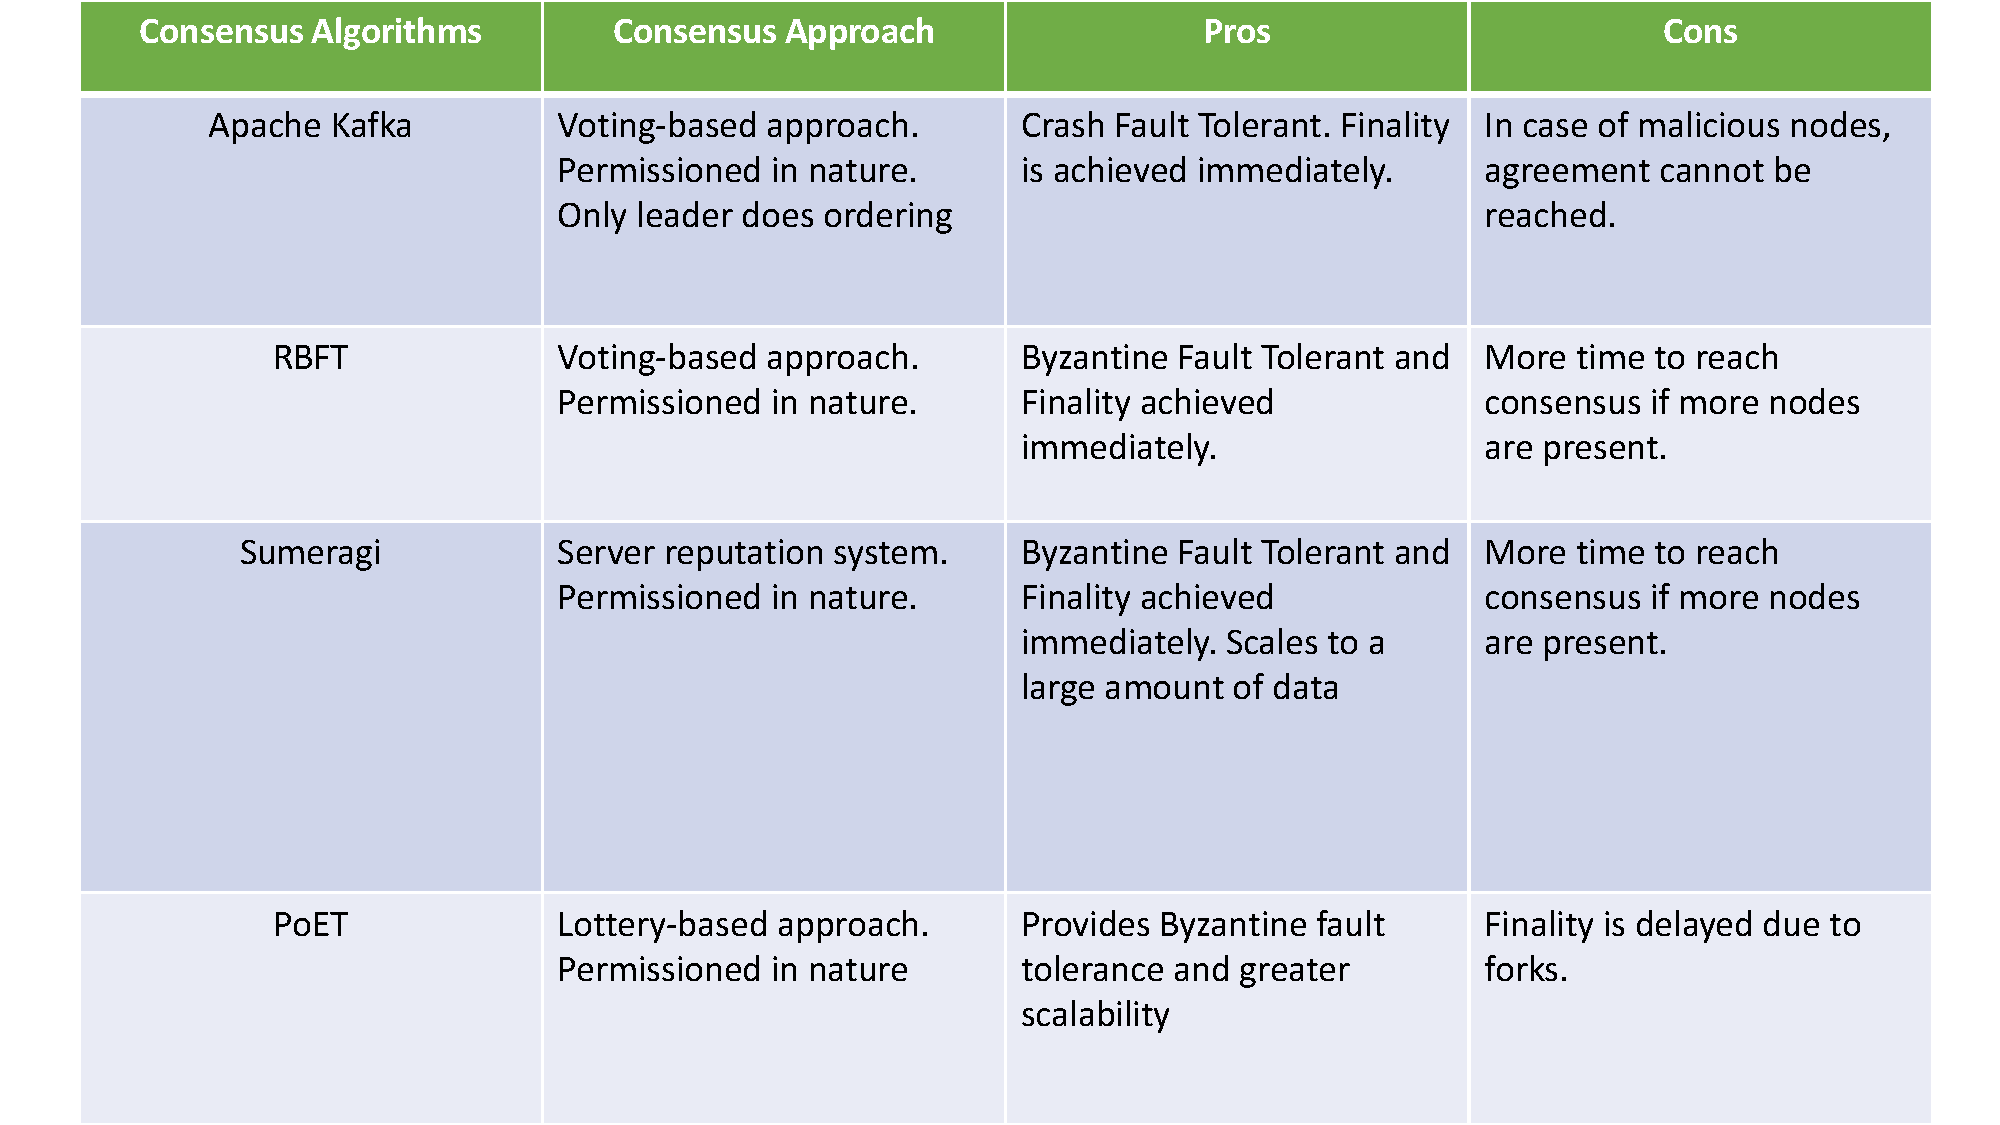
\includegraphics[width=\textwidth]{graphics/consensus.pdf}
\caption{Comparison of commonly used Consensus algorithms in Permissioned blockchains \cite{HW1}}.
\label{fig:consen}
\end{center}
\end{figure}

\subsubsection{Consensus Properties}
The consensus protocols must always satisfy two important properties among the peers: \textbf{safety} and \textbf{liveness} \cite{HW1}.
\begin{enumerate}
\item \textbf{Safety}: Safety property of any consensus algorithm ensures deterministic results on all the nodes. A transaction is called as deterministic if the same operation performed across different peers returns the same output no matter the time and order of execution. Safety property ensures that the algorithm behaves like a single node system that executes and validates transactions atomically and one at a time \cite{HW1}.

\item \textbf{Liveness}: Liveness is an important property that deals with the eventual delivery of transactions. It ensures that every non-faulty peer in the system will receive the transaction at one point of time or the other given that the communication mechanism is not down and the system can synchronize in case of failures \cite{HW1}.
\end{enumerate}



\subsection{Membership Service Provider (MSP)}
In a permissioned blockchain network, every participating entity is assigned a unique identity. This identity is wrapped around in an X.509 digital certificate \cite{Identity}. With the help of these identities, the permissioned blockchain network decides who has the proper rights and authorization to submit a transaction or who can access the resources. An \gls{msp} defines the Root \glspl{ca} and intermediate \glspl{ca} of a blockchain trust network. In a permissioned blockchain scenario, an organization is the trusted entity \cite{Membership}. An \gls{msp} also defines the access rights for different participants of the network and the channel. For e.g. some peers in a Hyperledger Fabric network may only have read access and no write access to the ledger. This is taken care by the \gls{msp}. The \gls{msp} configuration is available on the channels as well as on the peers, orderers, clients to authenticate a member outside the context of the channel \cite{Membership}.

\subsubsection{Channel and Local \glspl{msp}}
\glspl{msp} can be either present on the channel configuration information and is called as \textit{channel \gls{msp}} or it may be present locally on the peer, orderer or the client and is called as a \textit{local \gls{msp}}. In case of peers and orderers, the \gls{msp} defines the access privileges for them whereas in case of the client the \gls{msp} allows to identify the user in the transactions on the channel or if the user has a specific role like \textit{admin} in the system \cite{Membership}. 

\begin{figure}[t!]
\begin{center}
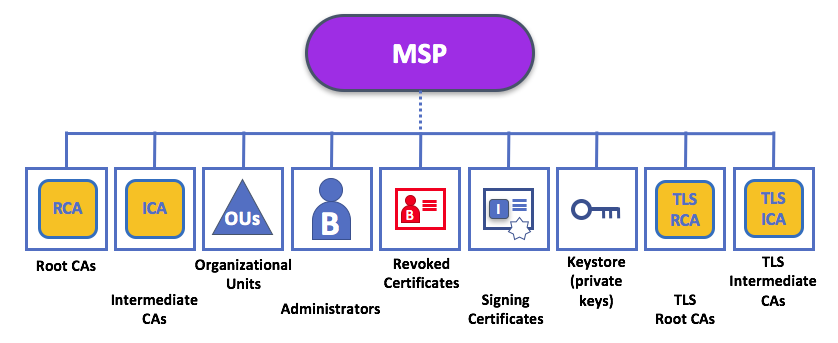
\includegraphics[width=\textwidth]{mem.png}
\caption{Figure showing how a local MSP is stored on a local file system \cite{Membership}}.
\label{fig:mem}
\end{center}
\end{figure}

\subsubsection{\gls{msp} Structure}
In addition to the root or intermediate \glspl{ca}, there are many other important aspects in a membership for the organization. Figure \ref{fig:mem} shows the local \gls{msp} structure on a local file system. The importance of the various components of an \gls{msp} can be described as follows:
\begin{itemize}
  \item \textbf{Root \glspl{ca}}: This is an important folder in the \gls{msp} file system that contains the X.509 certificates of the Root \glspl{ca} that is related to the organization's \gls{msp}. From the Root \glspl{ca} all other certificates for other members are derived \cite{Membership}.
  \item \textbf{Intermediate \glspl{ca}}: This is a folder on the local \gls{msp} file system that contains the X.509 certificates of the intermediate \glspl{ca}. The intermediate \gls{ca} certificate has to be signed by at least one of the Root \glspl{ca} of that organization. The intermediate \gls{ca} is important when a particular organization is part of a larger blockchain network and where it has more than one subdivisions. For e.g. \textit{Org1} can have two subdivisions as \textit{Org1-Manufacturer} and \textit{Org1-Supplier}. Depending upon the channel on which the organization is present, it can take a particular subdivision role and the intermediate \gls{ca} for that subdivision is then used to issue certificates to the members of the organization on the channel \cite{Membership}.
  \item \textbf{\glspl{ou}}: The \glspl{ou} provide a list of the organizational units that are the members of the network and represented by the organization issuing the \gls{msp}. This is useful when the members of an organization have to be restricted to be having a particular identity signed by the designated \glspl{ca}. The \glspl{ou} specification is optional and if its is not specified, all the identities identified by the Root \gls{ca} and Intermediate \gls{ca} will become the members of the organization with the write privileges \cite{Membership}.
  \item \textbf{Administrators}: There is a folder for the administrators in the local \gls{msp} that defines the administrator identity for a given organization represented by the specific \gls{msp}. Generally, at least one administrator identity should be defined for an organization. The admin rights are not with the management of resources but it is determined by the specific policies used for the managing the system resources. For example, the policy of the channel may define that \textit{Org1-Manufacturer} administrator has the rights to add new organizations to a channel and the \textit{Org1-Supplier} has no such administrator rights. The \textbf{Role} attribute is also defined in the X.509 certificate as admin. The role is strictly within the organization and not on the entire blockchain network \cite{Membership}.
  \item \textbf{Revoked Certificates}: The identifying information about a revoked identity in a network is held in this folder. This contains a pair of strings known as Subject Key Identifier (SKI) and Authority Access Identifier (AKI). The administrator of an organization has the responsibility to advertise the updated Certificate Revocation List (CRL) to revoke an actor of its rights in the network \cite{Membership}.
  \item \textbf{Node Identity}: This folder contains the identifying information for the nodes or peers in the blockchain network. This is used whenever a node sends a transaction proposal for endorsement, the signed endorsed transaction response and when a node wants to commit the transaction or block on the blockchain. This is a mandatory folder for the local \glspl{msp} and there should be exactly one X.509 certificate for the peer \cite{Membership}.
  \item \textbf{KeyStore for Private Key}: This folder contains the node's \textit{signing key}. The \textit{signing key} is used as an identifier for the node whenever a transaction response is signed by the node. This signature is then used by other nodes in the network to verify the authenticity of the transaction result at the endorsement phase. This is a mandatory folder for the local \glspl{msp}. Channel \glspl{msp} do not have this folder as the main aim of channel \glspl{msp} is to work on the validation and not on verification of signing by the nodes \cite{Membership}.
  \item \textbf{TLS Root CA}: This folder contains the X.509 certificates of the Root \glspl{ca} for TLS communications. This is important in case the nodes want to communicate with each other regarding the ledger updates and when new nodes want to securely join the channel. It is mandatory to have at least one TLS Root \gls{ca} X.509 certificate in the respective folder \cite{Membership}.
  \item \textbf{TLS Intermediate CA}: This folder contains the X.509 certificates of the Intermediate \glspl{ca} for TLS communications. It is important when there is a need of commercial \glspl{ca} for generating TLS certificates of an organization. This is an optional attribute and can remain empty \cite{Membership}.
\end{itemize}

\subsection{Chaincodes}
Chaincodes are the programs that contain the actual business logic of the blockchain application and it is used to access the \textit{world state} data of the blockchain. Chaincode is similar to a \textit{Smart Contract} in Ethereum or a \textit{Stored Procedure} in the traditional \glspl{rdbms} \cite{HF}. It is a self executing piece of code that is installed and instantiated on the peers of a Hyperledger Fabric channel. The client application invokes the various chaincode functions by interfacing it with a network peer. The transactions executed by the chaincode are checked for validation by the committing peers and upon complete validation the transactions results from a chaincode execution are used to update the shared ledger and change the world state. Currently, Hyperledger Fabric supports different programming languages in which chaincode can be written. These includes \textit{Go}, \textit{node.js} or \textit{Java}. Chaincode has its own secure docker environment that runs loosely coupled from the corresponding peer containers \cite{HF}. The state generated by a chaincode cannot be directly accessed by a different chaincode. If the chaincodes are in the same network, the state of chaincode can be accessed with right permissions \cite{Chaincode}. 

\subsubsection{Types of chaincodes in Hyperledger Fabric}
\begin{itemize}
    \item \textbf{System chaincode}: Transactions like the chaincode lifecycle management and and Fabric policy configuration are handled by some special system transactions executed by the \textit{System chaincodes} \cite{HW2}. The System chaincodes can also be used to specify the application requirements depending upon the requirements of the network and the chaincode developers can program it according to the needs of the application. The \textit{\gls{escc}} is a special system chaincodes that handle the endorsement related transactions. The \gls{escc} takes a transaction proposal and the result as input and produces a response with the results and the endorsement signature \cite{HF}. The \textit{\gls{vscc}} is responsible for checking the validity of the transaction. It takes the input as transaction and the output is a response indicating if the transaction is valid or not \cite{HF}. There is also a \textit{\gls{mvcc}} that checks for the versions of the key-value store before committing it to the world state. This is especially useful to avoid \textit{double-spending}.
    \item \textbf{Application chaincode}: The applications states on the distributed ledger is maintained by the application chaincode that includes assets, data records or funds \cite{HW2}. The client invokes the application chaincode methods with the help of the API and submit a request for transaction. Every transaction is associated with a transaction ID that is stored in the append only ledger.
\end{itemize}

\subsubsection{Chaincode usage scenarios}
There are generally two different ways to define and develop chaincodes for the Hyperledger Fabric architecture:
\begin{itemize}
    \item \textbf{Using chaincodes to design business contracts}: The chaincode can be used as a standalone application instance that gets invoked automatically when a condition is met or it can be programmed and accessed with the help of an API and called from the client application whenever required \cite{HW2}.
    \item \textbf{Using chaincodes to manage assets in a network}: Chaincodes can be used to transfer the assets in a network between the participants. Account balances can be encoded into past transactions records and it is called as the \gls{utxo} model that is stateless. Chaincodes can also use the ledger state to store the asset value and its current holder and regularly modifying the world state as the asset moves in the network \cite{HW2}.
\end{itemize}

\subsection{Endorsement Policy}
Endorsement policy is defined on the chaincode and it states the set of peers or nodes on a particular channel that have to execute the the chaincode method and endorse the results obtained from execution for the transaction to be deemed as valid. It is a way of defining which organizations have to approve of a result before finally appending it to the ledger and modifying the world state \cite{Endorsement}. It is the responsibility of the validating peers to check for the appropriate number of endorsements for a transaction from the right sources as defined in the endorsement policy. The validating peers also checks for the signatures of peers in the endorsement for authenticity and authorization.
\begin{Listing}
  \begin{lstlisting}
peer chaincode instantiate -C <channelid> -n cc -P "OR('Org1.member', 'Org2.member')"
\end{lstlisting}
  \caption{Endorsement policy specification at the time of chaincode instantiation.}
  \label{lst:endo}
\end{Listing}
\subsubsection{Endorsement policy types}
Generally, endorsement is defined at the time of chaincode instantiation or upgrade and it common for all the functions of the chaincode execution. However, there are some instances where a more sophisticated endorsement policy has to defined at the key level. Lets us see the difference between the two
\begin{itemize}
    \item \textbf{Chaincode level endorsement policies}: When the chaincode is instantiated on a channel, it is possible to define the endorsement policy for that chaincode on that specific channel. It is specified with the \textbf{-P} switch in the CLI command. Listing \ref{lst:endo} shows the sample CLI command used to instantiate the chaincode on a channel with the endorsement policy specified with a \textbf{-P} switch. The command specifies that a chaincode with name \textit{cc} will be deployed on the peer and channel specified by the \textit{channelid} with an endorsement policy \textit{'Org1.member', 'Org2.member'}. This endorsement policy states that the transaction on the channel has to be either endorsed by a member of organization \textit{Org1} or \textit{Org2}. Whenever a new organization is added to the network channel, the endorsement policy has to be modified \cite{Endorsement}.
    \item \textbf{Key-level endorsement policies}: The chaincode level endorsement policies are bound to the lifecycle of the chaincode. The key-level endorsement policies can be updated from within a chaincode function and is considered as a transaction. If there is no key-level endorsement policy present, the chaincode endorsement policies are executed in general. Even if the key-level endorsement policy is present, the transaction to create a key-level endorsement policy has to met the chaincode endorsement policy specification. If a transaction involves modification of a key containing a key-level endorsement policy, the key-level policy will override the chaincode level policies. A particular key can have multiple key-level endorsement policies and all of them have to be satisfied for key update \cite{Endorsement}. 
\end{itemize}
\subsubsection{Roles in endorsement policy}
The endorsement policies are always specified in combination with the \glspl{msp} and the role of different nodes in the network. In general it takes the form \textit{'MSP.ROLE'} where MSP defines the associated MSP ID in the network and ROLE represents the associated roles with the \gls{msp} in the network \cite{Endorsement}. Some examples are:
\begin{itemize}
\item \textbf{'Org1.admin'}: This specifies the administrator of organization \textit{Org1} MSP.
\item \textbf{'Org2.member'}: This specifies any member of organization \textit{Org2} MSP.
\item \textbf{'Org3.client'}: This specifies any client of organization \textit{Org3} MSP.
\item \textbf{'Org4.peer'}: This specifies any peer of organization \textit{Org4} MSP.
\end{itemize}

\subsubsection{Syntax of the language}
There is a way of defining the policy in combination with the roles and the msp and a principal like \textit{AND}, \textit{OR} and \textit{OutOf}. Some examples are:
\begin{itemize}
\item \textbf{AND('Org2.peer', 'Org3.peer')}: This specifies that at least one signature from both the organization's peers.
\item \textbf{OR('Org2.peer', 'Org3.peer')}: This specifies that at least one signature from any one of the organization's peers.
\item \textbf{OutOf(1, 'Org2.peer', 'Org3.peer')}: This specifies that at least one signature from any one of the organization's peers. Similar to \textit{OR} policy in this case.
\end{itemize}

\begin{figure}[t!]
\begin{center}
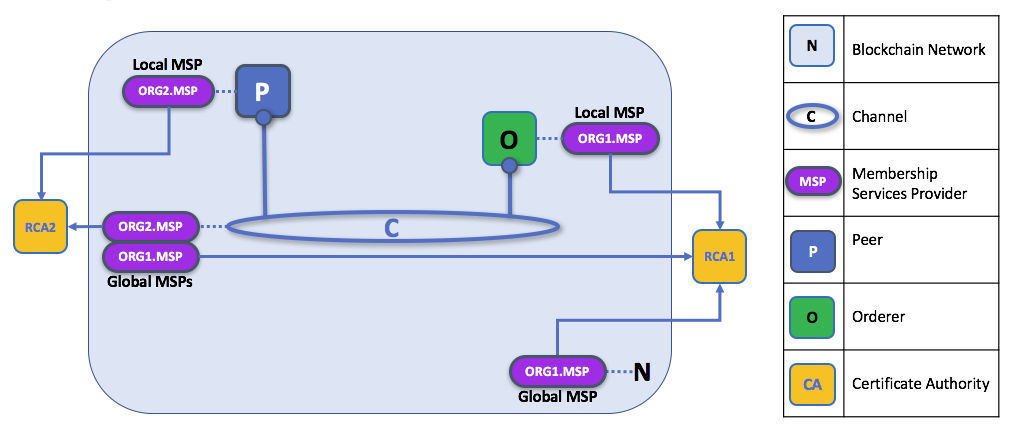
\includegraphics[width=\textwidth]{channel.png}
\caption{Figure showing a blockchain network with two organizations, their corresponding MSP, the peer, the orderer and the channel \cite{Membership}}.
\label{fig:channel}
\end{center}
\end{figure}

\subsection{Channels}
Hyperledger Fabric has the channel capabilities for a subset of participants in a blockchain network to provide some form of confidentiality and privacy. Channels are a useful feature when there are competitors involved on the same blockchain network and they do not want to share any sensitive information that might undermine their business profits. The shared ledger, chaincode applications, the ordering service node(s), members of the organization and the anchor peers per member define the channel. The transactions are checked for authentication and authorization on the channel where they are executed. The channel identifies each peer joining the channel by the \gls{msp} of that organization to authenticate it \cite{Channels}.

The client SDK calls the configuration system chaincode and checks the properties like the anchor peers, members of the organizations to create a new channel. The first step in channel creation is the generation of a genesis block for the common channel ledger. The genesis block stores the channel configuration information about the channel members, anchor peers and the endorsement policies. When a new member is added to an existing channel, the genesis block containing all the required information is shared with the new member \cite{Channels}. Figure \ref{fig:channel} shows a typical channel created for the two organizations. The peers that are part of this channel can submit and invoke transactions on the channel ledger. Listing \ref{lst:chan} shows the sample peer commands that can be used to create a channel and join the peer to the channel \cite{Channels}.

It is not possible to pass data from one channel to another which is secured by configuration chaincode, the gossip data dissemination protocol and the identity membership service. Channels are similar to the private access modifiers in a object oriented class providing access only to the right members of the channels. It is however important to note that chaincodes can be called from different channels but only for querying and it cannot be used for updating the ledger.
\begin{Listing}
  \begin{lstlisting}
peer channel create -o <ordering-service url> -c <channelName> -f <channel.tx file> --cafile<path to the peer identity file>
    
peer channel join -b <genesis-block.block>
\end{lstlisting}
  \caption{Different peer commands to create a channel and to join the peer to the created channel \cite{Channels}.}
  \label{lst:chan}
\end{Listing}

\begin{figure}[h!]
\begin{center}
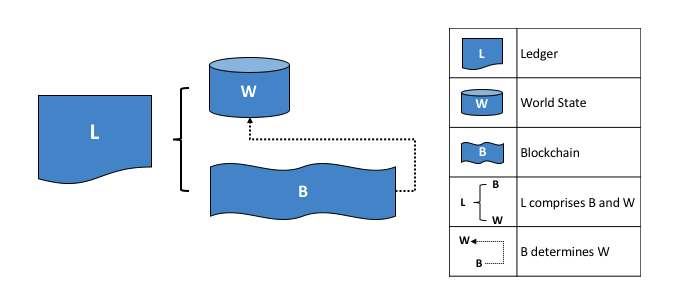
\includegraphics[width=\textwidth]{ledger.png}
\caption{Figure showing a Ledger consisting of the world state and the blockchain \cite{Ledger}}.
\label{figure:ledger}
\end{center}
\end{figure}

\subsection{Ledger}
The Ledger in Hyperledger Fabric consists of two different components, the \textbf{world state} and the \textbf{blockchain}. The world state holds the current value of a key. So whenever a new transaction is invoked and if it is successful the world state gets updated with the value obtained in the transaction execution. Whenever a peer queries the chaincode for a key value, the queries are run against the world state to give the result back. The world state is stored as a key-value pair dataset. The blockchain contains the history of all the transactions and can be considered as an historical log. The world state can be generated any time by traversing the entire blockchain. It is immutable and once transactions are appended they cannot be modified \cite{Ledger} \cite{HF}. Figure \ref{figure:ledger} shows a Ledger L comprising of a world state W and the blockchain B. The world state W can always be generated from the blockchain B. The different members of a blockchain network contain the same consistent copy of the ledger.

\subsubsection{World State}
World state contains the current value for any key and can be accessed from the chaincode without the need to traverse the entire history of the blockchain. The chaincodes can access the world state key values and modify it with the API interfaces like \textbf{GetState}, \textbf{PutState} and \textbf{DeleteState}. The state values can be either simple with just a single value like \textit{\{key=Vehicle1, value="Truck"\}} or complex consisting of multiple value fields like \textit{\{key=Vehicle1, value=\{type:"2-wheeler", color:"red"\}\}}. 

It is important to note that only those transactions that have the required number of endorsements as per the endorsement policy can change the world state. The state or the key-value pair are always associated with a version number. Every time a key gets updated, its version number gets incremented by 1. Initially when a ledger is created the world state is empty and subsequently gets populated when transactions are endorsed and committed in the blockchain\cite{Ledger}.

\begin{figure}[b!]
\begin{center}
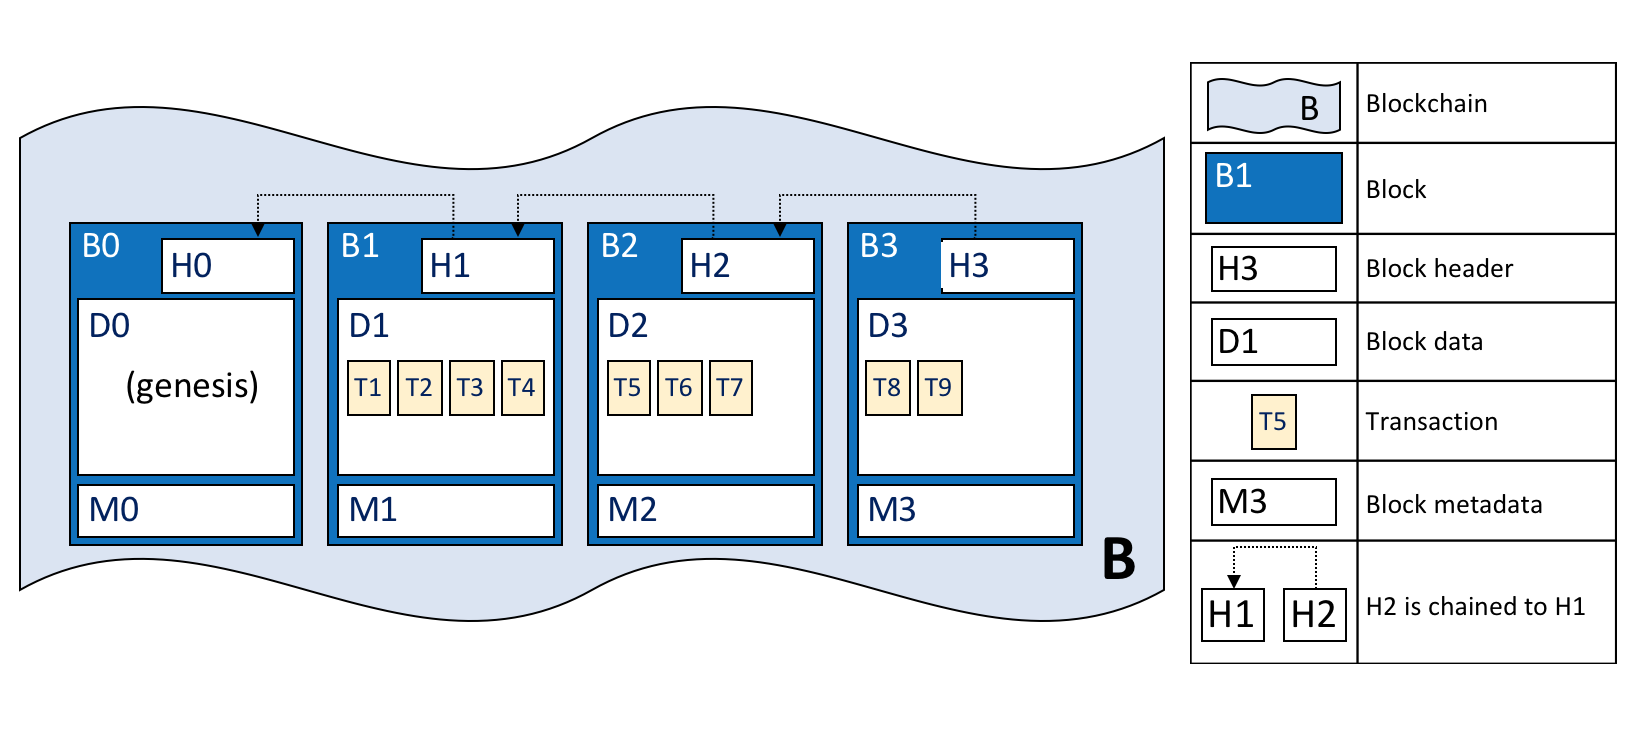
\includegraphics[width=\textwidth]{blockchain.png}
\caption{Figure showing the structure of the blockchain ledger \cite{Ledger}}.
\label{fig:blockchain}
\end{center}
\end{figure}

\subsubsection{Blockchain}
The blockchain part of the ledger contains the history of transaction logs and it is considered as append only and immutable. The blocks in the blockchain are interlinked with each block containing a sequence of transactions. The block's header includes a hash of the previous block header and the hash of all the transactions in the block. This hashing makes the blockchain secure and tampering can be easily detected as the blockchain itself is distributed. The world state is implemented as a database whereas the blockchain is designed as a file. Since, its append only, the file structure is much more appropriate \cite{Ledger}.

Figure \ref{fig:blockchain} shows the typical blockchain file structure consisting of interlinked blocks. It states that the Blockchain B is composed of blocks B0, B1, B2, B3. B0 is the genesis block in the network that contains configuration transaction and is the starting point of the blockchain. The block B3 contains block data D3 consisting of all the transactions T8 and T9. Header H3 of block B3 contains the hash of transactions T8 and T9 as well as the hash of the previous block B2's header H2.


\subsection{Data storage}
As discussed in the previous section, the world state is implemented as a database unlike the file system of the blockchain. The world state key values can be simple or complex and Hyperledger Fabric provides two different database options for the world state : \textit{LevelDB} \cite{ldb} and \textit{CouchDB} \cite{cdb}.

\subsubsection{LevelDB}
LevelDB is the default data store in Hyperledger Fabric and it is embedded within the peer operating system process. In other words, it is tightly coupled with the peer process and its life cycle is associated with the peer node. It is especially useful when the ledger states are simple key-value pairs \cite{Ledger}.

\subsubsection{CouchDB}
CouchDB supports rich and complex queries and supports simple datatypes and JSON documents for the ledger states. As a result CouchDB cab be used for efficient queries that is the main requirement of a business transaction. It runs in a separate environment than the peer operating system process but has a one to one mapping with the corresponding peer process.

Thus with the requirements of the business, different databases can be implemented as a relational data store, temporal data store or a graph structure. Hyperledger Fabric provides pluggable data store functionality \cite{Ledger}.
\section{Hyperledger Sawtooth as Permissioned Blockchain Network}
Hyperledger Sawtooth is a part of the Hyperledger group of projects hosted by the Linux Foundation. It is designed particularly for enterprise use due to its modular design that allows the applications to choose access control, transaction rules and consensus mechanisms in the blockchain network \cite{saw}. 
\subsection{Characteristics of Hyperledger Sawtooth}
\begin{enumerate}
    \item \textbf{Clear separation between the core system and application}: Sawtooth provides a smart contract abstraction layer that facilitates the applications developers to use a language of their choice to develop the smart contracts \cite{saw}.
    \item \textbf{Private groups with access control}: Separate access control can be specified for a group of nodes as the blockchain maintains stores the configuration information for access control for all participants to quickly access it \cite{saw}.
    \item \textbf{Parallel transaction execution}: With the help of a parallel scheduler, Sawtooth executes transactions parallely while still taking into consideration the transaction dependencies \cite{saw}.
    \item \textbf{Event system}: Sawtooth provides a way to subscribe to events so that the nodes can be notified \cite{saw}.
    \item \textbf{Pluggable consensus protocols}: Just like Fabric, Sawtooth also provided a pluggable mechanism to select the consensus algorithms depending upon the need of the network \cite{saw}.
    \item \textbf{Sample transaction families}: Just as Fabric has chaincodes, Sawtooth provided predefined transaction families and user-defined transaction transaction families as models. For example, the \textbf{IntegerKey} transaction family is used to test the deployed ledger \cite{saw}.
\end{enumerate}

\subsection{Transactions and Batches in Sawtooth}
In Sawtooth, transactions that are successfully executed result in state changes. Transactions are included in \textbf{batches}. A batch is an atomic unit of work in Hyperledger Sawtooth \cite{saw}. This implies that either all the transactions in a batch are committed or none at all.

\subsubsection{Dependencies between transactions}
There are instances when a transaction execution is dependent on the successful execution of some other transactions and this results in a form of \textit{dependency}. There is \textit{dependency} field in the transaction proposal in Sawtooth that specifies the dependent transaction \cite{saw}. This is called \textbf{explicit dependency} if it is specified by the client and allows two dependent transactions to be included in different batches but executed in right order. The parallel scheduler in Sawtooth takes care of \textbf{implicit dependencies} by interacting with the state. There is a input and output field in transaction proposal that specifies the address of the state \cite{saw}.

\subsubsection{Importance of batches}
Batches are the atomic unit of work in Sawtooth. If there is a invalid transaction in a batch, the batch is not applied and it is rejected. This helps to avoid the explicit dependency for transactions in the same batch as transactions are sequentially executed. External dependencies have to be specified only if the dependent transactions are in different batches \cite{saw}.

If there is a \textit{cyclic dependency} between the transactions, it cannot be solved with \textit{explicit dependency} specification at the transaction level. Suppose there are three transactions \textbf{X}, \textbf{Y}, \textbf{Z} that have to be applied in the same order. When a cyclic dependency is present between them, this cannot be defined with explicit dependencies alone. Batches solve this problem by executing the transactions in an ordered manner and rejecting the entire batch if any transaction fails. Dependencies specify the ordering of transaction execution and this fails in scenarios where there is a cyclic dependency as it cannot be specified in the transaction \cite{saw}.

\chapter{Related Work}
\label{chap:rel}
In this chapter, we will discuss the two important reference work done on blockchains related to the transaction characteristics analysis. These two are important as they highlight the differences between the permissionless and permissioned blockchain networks. In Section \ref{sec:1}, the permissionless blockchains are studied for their transactional properties. In Section \ref{sec:2}, Hyperledger Fabric and its underlying architecture is discussed which is used as a reference for further study in the thesis.

\section{A Transaction Processing Perspective on Blockchains}
\label{sec:1}
In this keynote paper, Tai et.al. discuss the transactions characteristics of blockchains \cite{Salt}. A different model called \textbf{SALT} is proposed for the blockchain transactions.

\subsection{Motivation}
The \glspl{rdbms} transactions focus on achieving database consistency while BASE is a model that trades some consistency for availability. With the introduction of blockchains that emphasize on distributed peer-to-peer technology and immutable ledger, another model in place ACID and BASE has to be introduced as blockchain transactions are consensus driven.This model introduced by Tai et.al. is called as SALT \cite{Salt}.

\subsection{Study Approach}
Blockchain transactions are consensus driven and have different properties compared to ACID and BASE models. Blocks contain transactions and it is important to study the blockchains from transaction perspective as well as block or system perspective. In this study, two real world application example of blockchain are used for comparison and evaluation of transaction properties. One use case involves Monegraph \cite{mon} which is an online digital media platform to share or sell media rights to different media users. The second use case uses Provenance blockchain \cite{pro} that is a supply chain traceability  application providing information about a product as it flows in the supply chain. 

Both the use cases were studied from a transaction and system perspective and the results were concurrent. The blockchain transactions were characterized as \textit{Sequential}, \textit{Agreed}, \textit{Ledgered} and \textit{Tamper-Resistant} from a transactions perspective. From a system perspective, these transactions were characterized as \textit{Symmetric}, \textit{Admin-free}, \textit{Ledgered} and \textit{Time-consensual} \cite{Salt}.

However, it is also important to note that the study was done on the permissionless blockchain networks and thus, it highlights the transactional properties of permissionless blockchains.

\section{Hyperledger Fabric: A distributed Operating System for Permissioned Blockchains}
\label{sec:2}
This paper describes the modular architecture of Hyperledger Fabric and its various components like consensus algorithms, smart contraction layer, transaction flow, peer communication, ledger, etc. With the help of this study, we get a deep understanding of permissioned blockchain network like Hyperledger Fabric.

\subsection{Motivation}
Androulaki et. al. describe the working of Fabric and its underlying architectural style and the programming setup required to build a permissioned blockchain model. Fabric is the first blockchain system that runs distributed applications without systemic dependency on a native cryptocurrency. This is quite opposite to the permissionless blockchains that require cryptocurrency for transaction execution. Fabric uses portable membership concept combined with identity management for access control. It uses the architectural model for transaction processing called as execute-order-validate model that removes non-determinism from the smart contracts. These properties make Fabric an ideal candidate for study related to the transaction processing \cite{HF}. 

\subsection{Study approach}
The study in this paper highlights the difference between the order-execute architecture model used in permissionless blockchains and early permissioned blockchains and the execute-order-validate architecture model of Hyperledger Fabric. For the purpose of study, a authority minted cryptocurrency similar to that of Bitcoin is used which is defined as \textit{Fabcoin} in the paper \cite{HF}. The study is focussed on the customization of the validation phase and the endorsement policy. The developed model is used for benchmarking of permissioned blockchains.

\section{Blockchain Consensus Protocols in the Wild}
Cachin and Vukoli\'c \cite{Con} wrote a paper on the different consensus models for blockchain that include crash tolerant and byzantine tolerant models.

\subsection{Motivation}
Blockchain transactions are based on consensus mechanism and it is essential to have an efficient consensus algorithm so that the transactions are secure and resilient. The main aim of consensus is to agree on the data and the order in which the transactions are executed. There are chances that a particular blockchain network can have adversarial nodes in the system and hence, a blockchain system should be able to tolerate Byzantine faults. 

\subsection{Study Approach}
Cachin and Vukoli\'c review the different consensus protocols in some prominent permissioned blockchain platforms and analyze their fault models and resilience against attacks. The protocol comparison covers Hyperledger Fabric, Tendermint, Symbiont, Iroha, Kadena, Chain,  Ripple, Stellar, and others \cite{Con}. Figure \ref{fig:conT} shows the consensus resilience properties in different blockchains.

\begin{figure}[h!]
\begin{center}
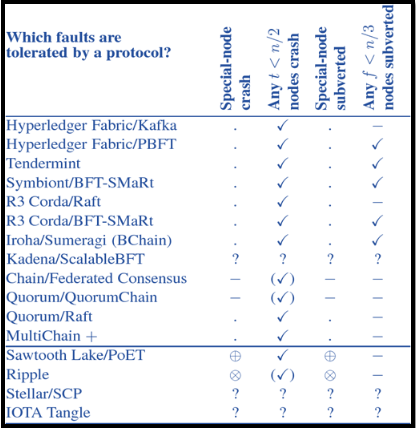
\includegraphics[width=10cm,height=10cm,keepaspectratio]{conTable.png}
\caption{Summary of consensus resilience properties, some of which use statically configured nodes
with a special role. Symbols and notes: ‘X’ means that the protocol is resilient against the fault and ‘−’
that it is not; ‘.’ states that no such special node exists in the protocol; ‘?’ denotes that the properties
cannot be assessed due to lack of information; (X) denotes the crash of other nodes, different from the
special node; + MultiChain has non-final decisions; ⊕ PoET assumes trusted hardware available from
only one vendor; ⊗ Ripple tolerates one of the five default Ripple-operated validators (special nodes) to
be subverted \cite{Con}}.
\label{fig:conT}
\end{center}
\end{figure}

\chapter{Blockchain Transaction Characteristics}
In this chapter, we will see the various transaction characteristics of permissioned blockchain network by studying the Hyperledger Fabric framework. We will compare the transaction properties of Hyperledger Fabric with that of the permissionless blockchain networks and the \glspl{rdbms} for a proper understanding. The effect of various components like \textit{channels}, \textit{chaincodes}, \textit{endorsement policies} and \textit{consensus algorithms} on the transaction properties will be studied here.
\label{chap:tc}

\section{Permissionless blockchain transaction properties}
Permissionless blockchains like Ethereum have been studied by comparing it to traditional \glspl{rdbms}'s ACID model and with the cloud systems and NoSQL data store's BASE model \cite{Salt}. The permissionless blockchains can be characterized as \textit{Sequential}, \textit{Agreed}, \textit{Ledgered}, and \textit{Tamper-resistant} from the transaction perspective, and as \textit{Symmetric}, \textit{Admin-free}, \textit{Ledgered}, and \textit{Time-consensual} from the transaction processing systems perspective \cite{Salt}. The focus of blockchain transactions is mainly on trustless transactions at the cost of scalability whereas ACID favors consistency at the cost of availability \cite{Tai}. the two perspectives of blockchains transactions can be described as in the below subsections. 

\subsection{Blockchain transactions-Transaction view}
As discussed before, permissionless blockchain transactions can be described as \textit{Sequential}, \textit{Agreed}, \textit{Ledgered} and \textit{Tamper-resistant} \cite{Salt}. Transactions are written on the blockchain and successful transactions update the world state of the ledger.

\subsubsection{Sequential}
The transactions in a blockchain network are executed sequentially. ACID transactions have the important characteristics of parallel transaction execution that increase the throughput of the system. However, in permissionless blockchains the transactions are not processed parallely and are only executed after one transaction finishes \cite{Salt}.

\subsubsection{Agreed}
In the ACID transactions, there is only one central authority that decides what data has to be added to the network. In permissionless blockchains, the transactions are added to the blocks and finally to the ledger after a consensus is achieved on the given transaction. The consensus can be reached in a variety of ways depending upon the type of consensus algorithm chosen and therefore, it is a distributed agreed transaction model \cite{Salt}.

\subsubsection{Ledgered}
The successful and consensual transactions are added to the blockchain and it cannot be tampered or changed. All the transactions are recorded in the blockchain and it is append only ledger that does not allow modifying a transaction once it is committed to the blockchain. It is also important to note that the Ledgered property is similar to the durability aspect of ACID transactions. \cite{Salt}.

\subsubsection{Tamper-resistant}
The blockchain is immutable and any effort to change the ledger can make the nodes aware of the tampering and it will be ultimately discarded. With the help of cryptography, transactions are signed by the crypto material or identity of the nodes and this helps the system to identify the right user who can submit a transaction. Furthermore, the blockchain is distributed among the network participants that work with consensus. Even if a node is compromised, other nodes in the system will discard the compromised data of the malicious or attacked node \cite{Salt}.

\subsection{Blockchain transactions-System view}
As discussed before the system perspective of permissionless blockchain transactions classifies it as \textit{Symmetric}, \textit{Admin-free}, \textit{Ledgered}, and \textit{Time-consensual} \cite{Salt}. Let us see the importance and meaning of these terms.

\subsubsection{Symmetric}
The peers in the permissionless blockchains symmetrically perform their responsibilities stating that every peer have the same processing tasks. This includes functions like data storage on the peer system, the transaction processing by signing the transactions and verifying the transactions and dissemination of information \cite{Salt}.

\subsubsection{Admin-free}
As blockchain is a peer-to-peer system and there is no administrator that has the responsibilities like network maintenance, access privileges or infrastructure management. These responsibilities are performed by all the nodes in the system in a consensual manner that helps to create a trust environment \cite{Salt}.

\subsubsection{Ledgered}
The nodes in a blockchain network maintain the ledger that is kept consistent on all the nodes with the help of the consensus property of blockchain. It is an append only transaction log that requires validation from all the nodes before adding a transaction in the logs. Blocks are a type of data structure that group transactions together. Consensus is generally reached on the blocks to reduce the number of consensus rounds and this block is then appended to the blockchain \cite{Salt}.

\subsubsection{Time-consensual}
The peers in a blockchain network may be geographically separated and hence, there is a high possibility that the blocks reach at different peers at different times. To solve this, the consensus algorithms defines an average time between which a new block can be created. This time is termed as \textit{block interval}. A transaction is therefore included into the ledger within half the block interval time but this is not guaranteed \cite{Salt}.

\section{Transaction Processing Models}
Initially, transactions in blockchain followed an \textit{order-execute} architectural style in which the network orders the transactions before sending them to all the peers in the network and then the peers execute all the transactions sequentially. The most important requirement of such a model is that it requires the transactions to be \textit{deterministic} \cite{HF}. Hyperledger Fabric follows a different architectural style for transaction processing and it is called as \textit{execute-order-validate} model \cite{HF}. In this model, the transactions are executed first, then the transactions are ordered with the help of a consensus algorithm and at the last the transactions are validated by the peers before committing it to the blockchain \cite{HF}. Let us see the details of the two models.

\subsection{Order-Execute Model}
In most blockchain networks, inclusive of permissionless and permissioned blockchains, the transaction processing model is based on the Order-Execute architectural style \cite{HF}. In this architectural style, the network first orders the transactions with the help of a consensus algorithm and then executes the transactions in the order in which they are processed on all the nodes in the network \cite{HF}. Different steps in a order-execute architecture are as follows:
\begin{enumerate}
    \item The nodes that participate in the consensus mechanism collects a block that contains valid transactions. The transactions are validated by the node itself by executing and verifying the results \cite{HF}.
    \item Depending upon the type of consensus protocol, the node or peer processes the valid transaction. For example, in \gls{pow} based system, the peer will solve a \gls{pow} mathematical problem \cite{HF}.
    \item The peer transmits the block to the network if it is successful in solving the mathematical problem.
    \item The other peers in the network that receive the block, validate the solution to the mathematical problem and also the transactions contained in the block. The receiving peers repeat the same execution steps as that carried out by the peer that solved the problem.
\end{enumerate}
All the peers execute the transactions in a block one after the other sequentially. The order-execute architecture is shown in Figure \ref{fig:oe}.

\subsubsection{Drawbacks of Order-Execute Model}
The order-execute is a simple architectural model but has many serious drawbacks associated with it which can be described as follows:
\begin{itemize}
    \item \textbf{Non-determinism}: Non-deterministic transactions are a major problem in the order-execute architectural style. In the order-execute model, consensus on the order of transaction is reached before the execution of the transactions. This involves that the transactions on all the peers produce deterministic results irrespective of the time of execution. If the transactions are non-deterministic, it can produce \textit{forks} in the blockchain and it is against the basic principle of blockchain that every peer holds the same copy of data. Determinism can be achieved by using a domain-specific programming language like Solidity \cite{HF}. 
    \item \textbf{Sequential transaction execution}: In a order-execute model all the peers execute the transactions in a sequential manner and this limits the overall throughput of the network to process the transactions. In addition, if a smart contract has some programming faults like an infinite loop, this can stop the entire blockchain network and proceeding transactions will remain halted forever. To solve this issue, permissionless blockchains like Ethereum use cryptocurrency to process a transaction. So even if the smart contract has programming error like an infinite loop, the cryptocurrency will get exhausted at some point of time \cite{HF}. In permissioned blockchains, this can be solved by executing the transactions in parallel. But in order to do this, transaction dependencies have to be considered before parallel transaction execution \cite{HF}.
    \item \textbf{Confidentiality of execution}: Most blockchain networks, run smart contracts on all the nodes in the network. But if the network requires confidentiality for the transaction, ledger state or smart contract logic, this becomes difficult to achieve without overloading the system \cite{HF}. The solution could be to create a network of trusted peers that execute the smart contract and propagate the results to other peers \cite{HF}.
\end{itemize}

\begin{figure}[t!]
\begin{center}
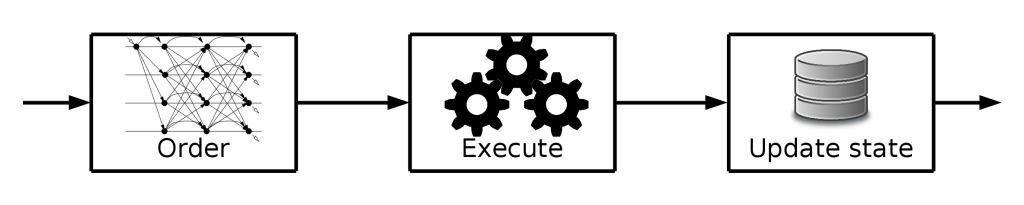
\includegraphics[width=\textwidth]{oe.png}
\caption{Figure showing the order-execute architectural style in blockchain network \cite{HF}}.
\label{fig:oe}
\end{center}
\end{figure}

\subsection{Execute-Order-Validate Model}
As seen in the previous subsection, the order-execute model suffers from a number of drawbacks that limits its application in the blockchain networks. This becomes very critical when business transactions are involved that have value only if executed in a secure and timely manner. To overcome the drawbacks in order-execute model, Hyperledger Fabric introduced the execute-order-validate model that solves all the major problems of the order-execute model \cite{HF}. Fabric has a smart contract called the \textit{chaincode} that performs the \textit{execution phase}. The transactions after execution are ordered by a \textit{ordering service} and this is called as the \textit{ordering phase}. In the \textit{validation phase} the ordered transactions are checked for the fulfillment of the endorsement policy \cite{HF}. Figure \ref{fig:eov} shows the transaction execution in Hyperledger Fabric by the execute-order-validate model. The importance of the three steps can be described as follows:

\begin{figure}[h!]
\begin{center}
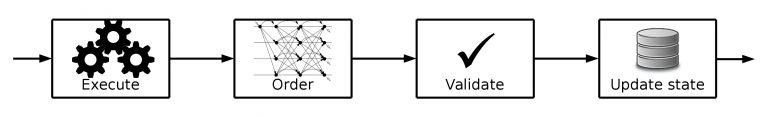
\includegraphics[width=\textwidth]{eov.png}
\caption{The execute-order-validate architecture model of transactions in Hyperledger Fabric \cite{HF}}.
\label{fig:eov}
\end{center}
\end{figure}

\subsubsection{Execution phase}
The client submits a transaction proposal by signing it to the endorsing peers in the network. The endorsing peers are specified at the time of chaincode instantiation on the channel. The transaction proposal submitted by the client contains the identifier of the chaincode, a counter or random variable, the transaction payload, parameters of the chaincode, a transaction identifier and the identity of the submitting client \cite{HF}. The chaincode is installed for the endorsing peers to generate the transaction results. This is called as creation of a \textit{proposal}. The proposal is generally executed against the local world state of the peer and the other peers have no knowledge about this state. The endorsers then produce a \textit{writeset} that consists of the keys and the new values of keys and a \textit{readset} that consists of the keys and its values read before endorsement. The signing of the message that contains the readset and the writeset is called as \textit{endorsement} that is delivered to the client as a response \cite{HF}.

Execution of the transaction before ordering them helps to overcome the drawback of non-deterministic chaincode. It is also possible to abort a transaction in case of \gls{dos} attacks that was not possible with the order-execute model \cite{HF}.

\subsubsection{Ordering phase}
The proposal response from the endorsing peers is collected by the client. As per the endorsement policy specification, the client waits till it gets the right number of valid responses and assembles a transaction and delivers it to the \textit{ordering service} for ordering. The transactions is composed of the endorsements, the chaincode methods with parameters and the metadata about the transactions \cite{HF}. Ordering is a process of atomically broadcasting \cite{ab} the endorsed transactions by establishing consensus on the transactions \cite{HF}. The ordering service does the work of putting transactions in blocks that helps to improve the throughput of the system \cite{HF}. The ordering service supports two operations:
\begin{itemize}
    \item \textit{broadcast(txn)}: This method is called by the client to broadcast a transaction \textit{txn} in the network. The transaction contains a payload and signature of the sending client \cite{HF}.
    \item  \textit{B\textleftarrow{}deliver(x)}: This operation is performed by the client on the orderer to retrieve a block B a sequence number as x. The block B contains a number of transactions that were included into it at the time of committing it to the ledger \cite{HF}.
\end{itemize}
It is the responsibility of the ordering service to ensure the blocks are fully ordered. It is important to note that the ordering service in Fabric does not execute or validate a transaction and it is concerned with the ordering of transactions. This makes the consensus process in Fabric quite modular by separating the execution and validation stages with the ordering stage \cite{HF}.

\subsubsection{Validation phase}
This is an important step before the blocks can be finally committed to the ledger. In this step the blocks are validated by the committing peers to check the content of the transactions within the block and the block itself. The steps in the validation stage are performed sequentially as: 
\begin{enumerate}
    \item \textit{Evaluation of endorsement policy}: This step involves parallel evaluation of the transactions in the block. The step is performed by the Validation System Chaincode \gls{vscc} that is responsible for checking the endorsement policy against the chaincode. The unsatisfied endorsements for a transaction results in the transaction becoming invalid but it is still included in the block and its effect does not take place on th ledger. It is logged for future auditing \cite{HF}.
    \item \textit{Read-write conflict check}: This is a sequential step that is done for all the transactions in the block. In this step, the key versions in the \textit{readset} is compared with the current version of the key in the ledger state. Non-matching versions result in invalid transactions and its effect on the ledger is prohibited \cite{HF}.
    \item \textit{Ledger update stage}: This is the last step in which the block is finally appended to the ledger and the world state is also updated with the new key values. The state changes are done by updating the key values with the \textit{writeset} of the valid transactions. Invalid transactions are still included in the block but have no effect on the world state \cite{HF}.
\end{enumerate}
The result of the validation stage may also contain invalid transactions in the block. This is very useful in cases when the auditing is done to identify peers that submitted faulty transactions.  


\section{Transaction flow in Hyperledger Fabric}
Hyperledger Fabric follows a execute-order-validate architecture to overcome the drawbacks present in the order-execute architectural model of transaction processing. Transactions in Fabric can be either \textit{Deploy transactions} that create a new chaincode for the specified peer or \textit{Invoke transactions} that perform a particular operation on a already installed chaincode. The execution may result in modification of world state because of \textit{write} or just a simple query to return a key value (read). Figure \ref{fig:tf} shows a typical transaction flow from execution, ordering to the validation of transactions in Hyperledger Fabric. The steps can be outlined as below:
\begin{enumerate}
    \item The client submits a transaction request that is passed to all the endorsing peers in the blockchain network. The transaction proposal is composed of the client identifier, chaincode identifier, transaction payload, timestamp and the client signature.
    \item The endorsing peers simulate the transactions and produce a transaction response. This process is called as \textit{endorsement} and is part of the \textit{execution phase}. The endorsing peers submit the proposal response to the requesting client.
    \item In this step, the client verifies the minimum amount of correct endorsements received on the transaction response and sends it to the ordering service to be included in the block and ultimately into the blockchain. The ordering service then orders the transactions as it receives in a sequence. This is called as \textit{ordering phase}.
    \item In the last step, the ordering service disseminates the blocks containing the transaction simulation results to all the peers in the network and optionally to the client. The peers validate the blocks and the transactions in the block that is finally appended in the ledger. This is called as \textit{validation phase}.
\end{enumerate}

\begin{figure}[t!]
\begin{center}
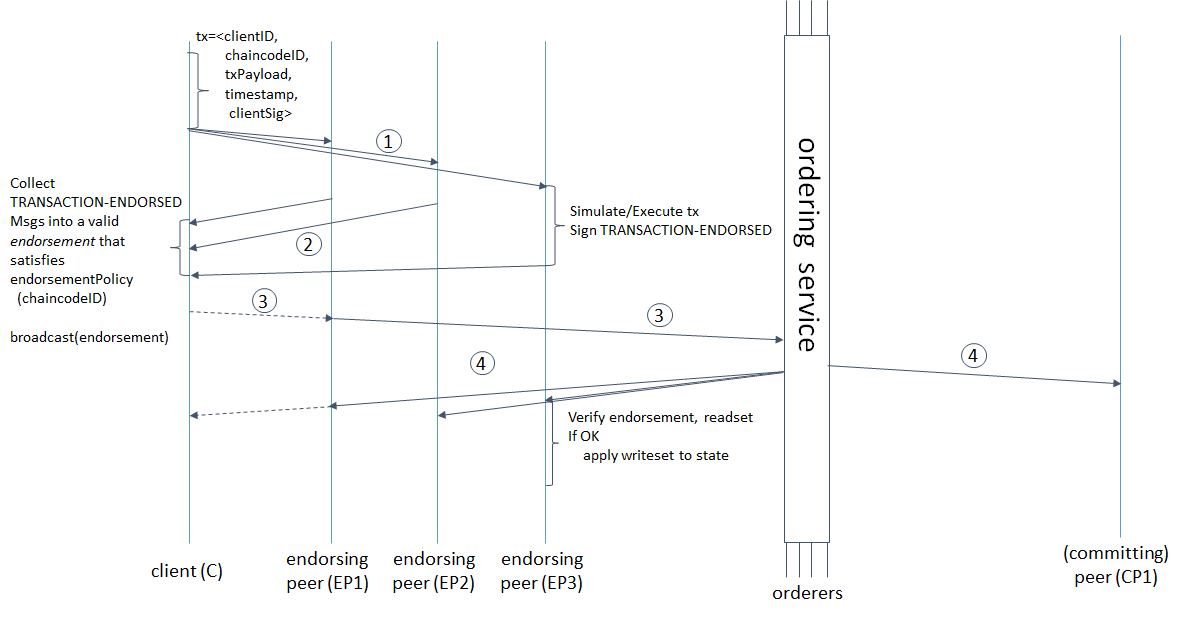
\includegraphics[width=\textwidth]{tf.png}
\caption{Transaction flow in Hyperledger Fabric that follows an execute-order-validate architectural style \cite{hfarc}}.
\label{fig:tf}
\end{center}
\end{figure}


\section{Hyperledger Fabric transactional properties from an ACID perspective}
We have already seen the transaction flow in Hyperledger Fabric. There are various aspects to consider that affect its transaction processing characteristics. In this section we will evaluate the transactional properties of Hyperledger Fabric from an ACID perspective both at the transaction level and at the system level or block level and also see ways by which the properties can be made stronger.

\subsection{Atomicity}
Atomicity is a property by which the \glspl{rdbms} guarantees that the transaction will either be committed fully or not committed at all \cite{Atomicity}. In blockchain, atomicity can be evaluated at the individual transaction level and at the block level.
\subsubsection{Transaction level atomicity}
Atomicity states that a transaction is either fully committed or not committed at all. In Fabric, a transaction can be either a query or invoke on the chaincode that may modify the world state. Proper number of endorsements on the transaction execution result is required by the endorsing peers specified with the endorsement policy in order for the transaction to be committed to the blockchain. If the endorsement is met, the transaction is sent to the orderer to be included in a block. On the other hand, if a transaction does not meet the endorsement policy specification, it not sent to the orderer.If a transaction fails the \textit{validation system check} and \textit{multiversion system check}, it is marked as invalid but it is not removed from the block and still appended to the blockchain but the world state is not updated. This is different from the permissionless blockchain networks where invalid transactions are not included in the block. Since, the state changes occur only if the transaction is valid, it can be considered as atomic. It is also important to note that if the endorsement criteria is not met, the transaction is not sent to the orderer to be included in the block and the transaction, therefore, does not commit making it \textit{atomic} \cite{HF}.

\subsubsection{Block level atomicity}
Once the transaction passes the endorsement criteria, it is sent to the ordering service to be included in the block. Blocks contain the transactions that have satisfied the endorsement policy. If, at the \textit{validation phase}, the transaction is deemed as invalid due to a version check failure or validation failure, it is not removed from the block but marked as valid. The generated block will always be committed to the blockchain. This makes the blocks \textit{non-atomic}.

Further work can be done to avoid committing a block in which all the transactions are invalid. This would keep the blockchain short.

\subsubsection{Guarantee of Atomicity}
There are scenarios in business transactions, where one transaction might be dependent on some other transaction. \textit{Transaction dependencies} should be taken care of so that the transactions execute in the right order. Endorsement policy should be strong enough so that valid transactions are included in the block. In some cases it might happen that a block contains two different transactions that write to the same key in the world state. In this scenario, if the transaction model is not properly implemented only the first transaction will be valid and the second one will be deemed as invalid. Thus strong endorsement policy and \textit{multiversion concurrency checks} and \textit{validation system checks} are required to provide high degree of atomicity.


\subsection{Consistency}
Consistency states that the total asset value before and after a transaction in a system is always the same and it satisfies all the constraints \cite{Atomicity}. In blockchains, consistency can be either \textit{weak}, \textit{eventual}, \textit{strong} or \textit{no consistency} at all depending upon the peer behaviour after transaction execution. As every peer hold the same copy of the ledger, but the update might take time due to geographical location of the peer or due to unavailability, consistency in blockchain can be considered as eventual consistency.

\subsubsection{Ways to make the transactions consistent}
\begin{itemize}
    \item \textbf{Removal of non-deterministic behaviour}: Non-determinism in blockchain results in different transaction results on different peers for the same transaction. This is against the basic rule of distributed applications where the same copy is maintained on all the peers. The non-determinism in blockchain can be removed by:
    \begin{enumerate}
        \item Using execute-order-validate model removes inconsistent states in the blockchain prior to ordering them in the block and provides high throughput by executing them in parallel \cite{HF}.
        \item Using a deterministic execution model like Ethereum \cite{evm} and use of a deterministic language like Solidity \cite{sol} that avoids non-determinism in smart contracts.
        \item Parameters that affect the determinism of smart contract execution should always be passed from the client. For example, timestamp should be generated from the smart contract but passed from the client as every peer will get the same timestamp.
        \item External API calls should be avoided which may result in non-deterministic execution results \cite{HW2}.
    \end{enumerate}
    \item \textbf{Avoid Forking}: \textit{Forking} in blockchain creates two different chains and leads to inconsistent state in the blockchain. This is usually solved by taking the longest chain as the legitimate blockchain. Using execute-order-validate model can remove inconsistent states early and avoids forking. Also avoiding \textit{lottery-based} consensus algorithms can help in avoiding forking in the chain \cite{HW1}.
\end{itemize}

\subsection{Isolation}
Isolation ensures that multiple transactions can take place parallely without resulting in an inconsistent state in the database. This is equivalent to the transaction result execution in sequential manner with the advantages of concurrency control. Isolation guarantees that the changes made by a transaction are only visible only after its written to the main memory \cite{Atomicity}.

\subsubsection{Ways to achieve Isolation}
Transaction dependencies should be taken care to guarantee strong Isolation property. Dependency is created when the execution result of one transaction is dependent on the execution of another transaction. This dependency can be handled by the smart contract as they handle the transaction execution logic. Dependencies can be either \textit{explicit} or \textit{implicit} \cite{HW2}. 

\textbf{Implicit} dependency has to be taken care of by the smart contract and it is very hard to achieve. This can be implemented by using \textit{mempool} of transactions and continuously applying different transactions till the required result is obtained. With \textbf{explicit} dependency, the client application or the user has to specify which transactions occur in which order. In simple words, the user has to wait till one transaction finishes, fetch the result from that transaction and use those results to simulate the dependent transaction \cite{HW2}.

Similarly, \textbf{dependency graph} also affect the order of transaction execution in a block. The dependency graph can be of two types, \textbf{cyclic} or \textbf{acyclic} \cite{HW2}. Consider a cyclic dependency between three transactions \textit{X}, \textit{Y} and \textit{Z} such that \textit{X} depends on \textit{Y}, \textit{Y} depends on \textit{Z} and \textit{Z} depends on \textit{X}. In this cyclic dependency, all the three transactions must be in the same block and design should be done in such a way that \textit{multiversion check} should execute all the transactions \cite{HW2}.

With the acyclic dependency, the transactions can be included in different blocks but care has to be taken about the sequence in which transactions are committed. Explicit references can also allow for parallel execution of non-dependent transactions included in the same block \cite{HW2}.

\subsection{Durability}
Durability is the property by which the transaction results are kept persistent on the system even if there is a crash or failure. This is achieved by saving the data on a physical memory on the system. In blockchain, the ledger is composed of the immutable blockchain and the constantly updated world state consisting of the key value store with increasing version number \cite{Ledger}. 

The blockchain in the ledger is a file on the peer system and every peer maintains a copy of the blockchain. Since, it is an append only data structure, it makes sense to use files for the blockchain. It consists of blocks that are linked to each other. It is important to note that since the transactions are validated before committing, there is no guarantee that an successfully executed transaction will change the world state but it will be written on the blockchain. This ensures \textit{strong durability} for transactions.

The world state on the other hand consists of keys and their corresponding latest values that are updated regularly. The peer query is run against the world state. The world state can have different implementations ranging from a relational database model, NoSQL database, JSON document. It is important to note here that a successfully executed transaction might fail the \textit{validity checks} and the world state will not be updated. Hence, there is a \textit{weak durability} in this case.

\begin{figure}[t!]
\begin{center}
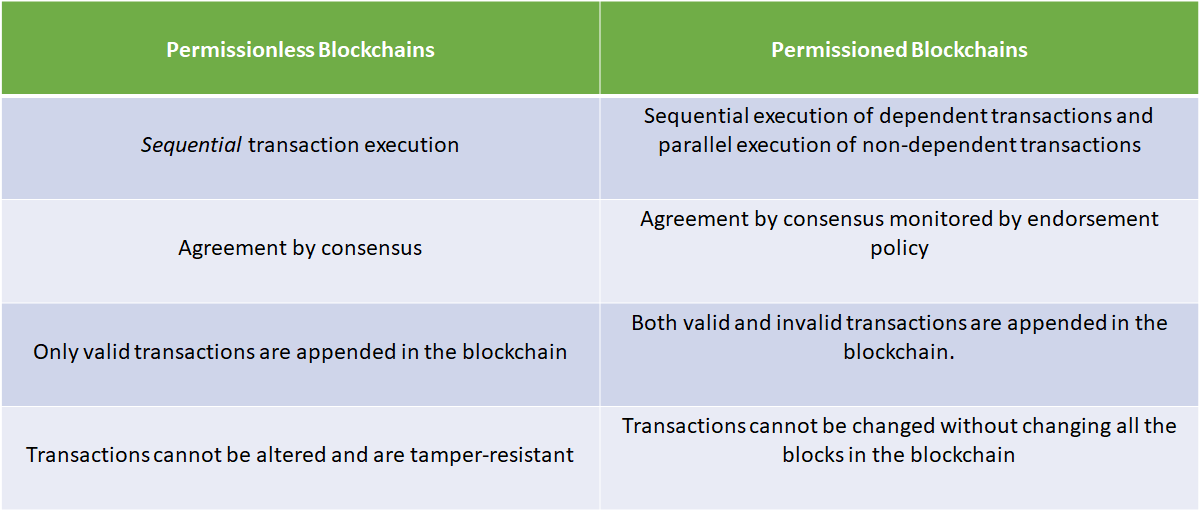
\includegraphics[width=\textwidth]{dif.png}
\caption{Differences in transactional properties of permissioned and permissionless blockchains at the transaction level.}.
\label{fig:dif}
\end{center}
\end{figure}

\section{Differences between Permissioned and Permissionless blockchains based on transactional properties}
The differences in the transactional properties of the two blockchain systems can be evaluated at the transaction level and at the block or system level. The main concept in both the blockchain networks is to have a peer-to-peer transaction processing system and having a distributed ledger that is secure and tamper-proof. Figure \ref{fig:dif} shows a table with differences from a transaction perspective. Permissionless blockchains can be considered as \textit{Sequential}, \textit{Agreed}, \textit{Ledgered} and \textit{Tamper-Resistant} at the transaction level \cite{Salt}. On the other hand, permissioned blockchains can be considered as \textit{Sequential and Conditionally Parallel}, \textit{Agreed and endorsed}, \textit{Ledgered} and \textit{Tamper-proof}. 

On the other hand at the block level, the transaction processing is a bit different. Figure \ref{fig:diff} shows the differences in transactional properties at the block level for the permissionless and permissioned networks. In permissionless networks, the transaction at the block level can be considered as \textit{Symmetric}, \textit{Admin-free}, \textit{Ledgered} and \textit{Time-consensual} \cite{Salt}. On the other hand, for permissioned blockchains \footnote{the reference is Hyperledger Fabric for the permissioned blockchains}, it can be considered as \textit{Asymmetric} due to different roles associated with an identity and access control, \textit{Admin-controlled} due to the presence of MSPs in the network for resource access, \textit{Ledgered} as both the valid and invalid transactions in a block are committed by the peer and \textit{Time-consensual} by defining a time-to-cut transaction by the \glspl{osn} in the network that creates deterministic blocks on all the nodes. This timer starts when a transaction is included in a block and when the timer expires and a block is still not cut, a time-to-cut transaction is broadcast to finish the block creation \cite{HF}.



\begin{figure}[h!]
\begin{center}
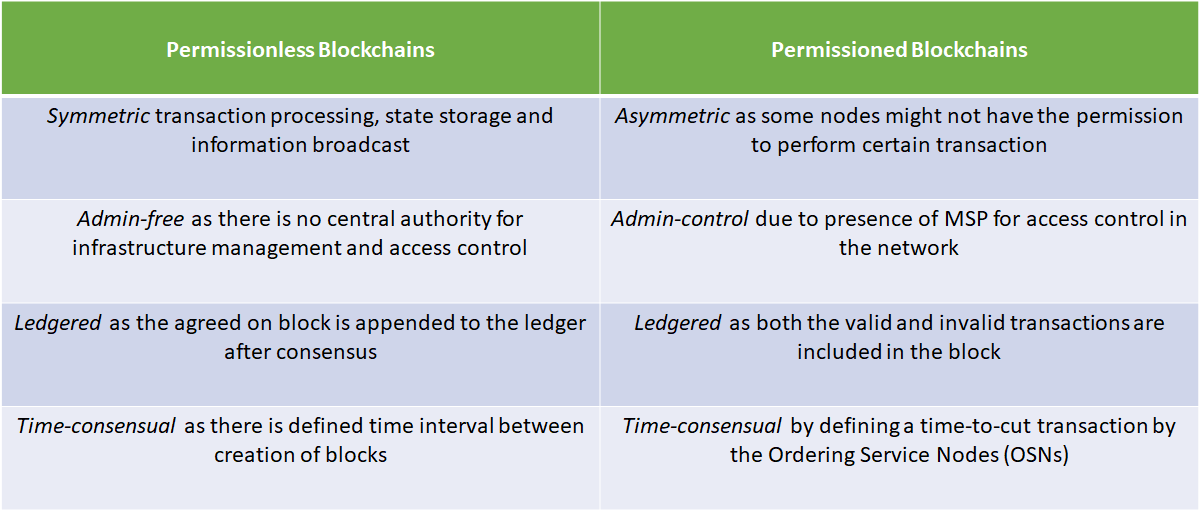
\includegraphics[width=\textwidth]{diff.png}
\caption{Differences in transactional properties of permissioned and permissionless blockchains at the block level.}.
\label{fig:diff}
\end{center}
\end{figure}

\section{Effect of consensus algorithms on transactional properties}
Consensus is a process by which the nodes in a blockchain network agree on the order and content of data. The peers in the blockchain network execute a \textit{consensus protocol} to create blocks from transactions, to validate the transactions and building a hash chain over the created blocks \cite{HF}. Therefore consensus is a necessary requirement to achieve \textbf{consistency} in the blockchain networks \cite{HF}.

The \textit{order-execute} architecture with the consensus implementation can lead to inconsistent state due to non-deterministic results \cite{HF}. In Hyperledger Fabric, the \textit{ordering phase} involves the use of consensus protocols for ordering the transactions in blocks \cite{HF}. Consensus also affects the \textbf{atomicity} of transactions specifying either a transaction execution result is valid or not. Only after the peers reach consensus on a transaction or block, it is considered valid and appended to the ledger by updating the world state. A strong consensus protocol can guarantee atomicity of transactions. 

\section{Effect of channels on transactional properties}
The concept of channels in Hyperldger Fabric provided confidentiality and privacy to the peers of the channel \cite{Channels}. However, since a business transaction can span different channels and be composed of many \textit{nested transactions} that are scattered over different channels, it is important to consider the impact of channels on transaction execution.

Having a channel is like creating a private blockchain network within a larger blockchain network. It can also be said that a blockchain network in Hyperledger Fabric is composed of several smaller channels. A peer can be on more than one channel but it maintains a separate ledger for the different channels. For example, if a peer \textit{P} is present on channel \textit{A} and channel \textit{B}, it will have two different ledgers \textit{L1} for channel \textit{A} and \textit{L2} for channel \textit{B}.

As the main purpose of channels is to isolate data, it becomes problem when a large business transaction involves sub-transactions from different channels. Consider that a chaincode call on one channel requires data from a chaincode call on a different channel (same chaincodes are installed on both the channels but their states are different). In this scenario, if the first transaction fails, the second transaction will not fail automatically and requires a layer of implementation on the top that handles this logic. Without proper implementation, the large transaction will be considered \textbf{non-atomic} and may result in \textbf{inconsistent state}. There are different ways to make the transactions consistent and atomic as:
\begin{enumerate}
    \item Use channels only when the data is not going to be used in different channels at all.
    \item Use of a single channel and private data collection to provide privacy for only the data that is sensitive and cannot be shared with other peers on the channel.
    \item Use of single channel with data encryption.
    \item Use of multiple channels with an intermediate implementation of a software layer like a 2-P transaction monitor on the application side that has access to all the channel's data and manages the dependent transactions. This layer has to take care of \textbf{rollback}, \textbf{compensation action} and \textbf{commit} for all the transactions. However, this type of implementation will make the network slow.
\end{enumerate}

\section{Effect of chaincodes on transactional properties}
Chaincodes contain the application logic for the entire blockchain network and for a peer to access the world state and ledger the chaincode has to be installed on the corresponding peer \cite{Chaincode}. A business transaction may span different chaincodes on same channel or on different channel. Proper transaction management has to be taken care of in such a scenario.

Chaincodes affect the \textbf{consistency} \textbf{isolation} and \textbf{atomicity} properties of a transaction and requires special effort on the side of the application developer to program the chaincodes in such a way that these properties can be guaranteed. Chaincode operations can be either \textbf{reads} or \textbf{writes}. This is also impacted by the introduction of a number of channels. Let us consider the different scenarios involving chaincode to chaincode call:
\begin{enumerate}
    \item \textbf{Same channel read operation}: It is possible to call a chaincode from another chaincode on the same channel to read the world state. This will be included in a single transaction and will respect the atomicity guarantee.
    \item \textbf{Different channel read operation}: Reads from a chaincode on a different channel are also possible. However, there is no MVCC check of the read value and the caller has to maintain the state in its own transaction context. If the caller has no access to the callee channel, the read will fail.
    \item \textbf{Same channel write operation}: The called chaincode has its own individual read write sets within the caller's transaction context. Therefor, committing this transaction will involve multiple chaincode's read-write sets on a single MVCC check.If there exists any key-version check failure from any involved chaincodes, the whole transaction will fail. This provides \textbf{atomicity} and \textbf{consistency} to the transactions \cite{jira}.
    \item \textbf{Different channel write operation}: The same transaction context cannot be used when different channels are involved. There are different ledgers involved with different key sets. In order to atomically co-ordinate the sub-transactions, the caller has to create an intermediate implementation like a 2-PC transaction monitor that handles all the sub-transactions in a single transaction context \cite{jira}.
\end{enumerate}

\section{Effect of endorsement policy on transactional properties}
Endorsement policies are defined at the time of instantiation of chaincode on a channel. A strong endorsement policy will guarantee \textbf{consistency} and \textbf{atomicity} of transactions. For example, if there are two organizations \textit{Org1} and \textit{Org2}, endorsement policy should be such that involves agreement on execution results from both the organizations. This can be achieved by using the policy \textit{AND(Org1.member, Org2.member)}. This will force the client to collect endorsements from both the organizations. The endorsement will be valid if and only if the peers sign the same bytes which will be different if the transaction results are different and will be easily caught. Thus a strong endorsement policy guarantees \textbf{consistency} and \textbf{atomicity} in the network.

\section{Other miscellaneous transaction terms}
In this section we will see some of the ACID transaction concepts in relation to the blockchain transactions and how they can be implemented.

\subsection{Peer transaction manager}
The traditional \glspl{rdbms} have a \textit{resource manager} that is responsible for affecting the state changes in the databases to maintain data consistency. In Hyperledger Fabric, the world state is maintained and managed by the \gls{ptm} \cite{HF}. The \gls{ptm} has a key-value store to manage the latest state in the form as (\textit{key, value, ver}) for every unique key of the chaincode state. The \textit{ver} in the store provides information about the sequence number of the block and also the transaction sequence number in the block. The version is unique and increases every time there is a state change \cite{HF}.

When a transaction is executed, its \textit{readset} in the form (key, ver) and writeset in the form (key, value) is maintained by the \gls{ptm}. The PTM also supports rich range queries by computing a hash of the query execution results and then adding the query string and hash in the \textit{readset} \cite{HF}.

The PTM also perform the validation phase to ensure consistency of data in the ledger. The validation of transactions is done sequentially in a block by comparing the version in the readset for a key to the latest version present in the blockchain. If the version differs, the PTM aborts the update of world state by marking the transaction as invalid. To avoid phantom reads for range queries, PTM executes the query again and compares the new hash with the one present in readset. In case of successful transactions, the PTM updates the latest state with the \textit{writeset} that it has \cite{HF}. Thus, PTM has the responsibility to maintain the integrity and consistency of transactions on all the peers respectively.

\subsection{Savepoint}
Savepoint is a way of defining labels or markers in a transaction so that if a failure occur, the transaction can be resumed from these labels \cite{sp}. It is a way of dividing a large complex transaction into smaller manageable transactions. In Hyperledger Fabric Ledger, the PTM is responsible for managing the \textit{savepoint} for the blockchain \cite{HF}. After the PTM validates the transactions and applies the state changes, it calculates the savepoint value that defines the largest successfully committed block number in the ledger \cite{HF}. This savepoint is very useful in times of crashes when the world state and the indices have to be recovered from the persisted blocks in the ledger \cite{HF}.

\subsection{Rollback transactions in Hyperledger Fabric}
Rollback is the process by which the transaction effects are undone in the context of transaction execution. As stated before, the blockchain is an append only data structure and the world state contains the latest value for a key. It is always possible to generate a world state from the blockchain with the help of \textit{savepoint} in case of crashes and with the help of mutual consensus in case the world state has to be regenerated for all the peers. However, rollback will not decrease the version number for a key in the world state and it will only increase with the rollback transaction.

\subsection{Compensating transactions}
In \gls{rdbms}, a compensating transaction is used when the transaction results are committed and have to be undone with a new transaction that overwrites it to the previous value or to some predefined required value. As discussed before, the ledger contains an append-only blockchain data structure and to create a compensation action a new transaction has to be submitted. This transaction will also be recorded in the blockchain and the world state can be updated with the required value.


\chapter{Concept, Specification and Design of a permissioned blockchain network}
\label{chap:cs}
In this chapter, we will create a blockchain network that works with a web application and an Android application. We will see the creation of different artifacts like the chaincodes, channels, endorsement policy, MSP, ledger, peer and client web applications and android applications that work with this blockchain network. Some of the experiments in Chapter \ref{chap:de} are based on the extension of this application. 

\section{System Overview}
We will create a simple supply chain application using Hyperledger Fabric that will help us to understand the transaction processing functions in permissioned blockchains. As a product passes hands through different parties in a supply chain, traceability of product regarding its authenticity and quality becomes troublesome and time-consuming. With the help of a blockchain application, all the interested parties are included in a single network and every participant maintains a copy of data. As a result, traceability becomes fast and it also provides transparency in the whole network. Moreover, it provides a trust environment for business transactions that was hitherto managed by third parties like banks.

The supply chain application can be used to trace any product from source to destination. For simplicity, we will not categorize the products and consider it as a general food product. The products, however, can be identified through their product id as we will show in our Android application. The supply chain involves participants like \textbf{supplier}, \textbf{producer}, \textbf{buyer} and \textbf{consumer} that we will depict in the application. The functions on a product will include \textit{query a product with its id}, \textit{query all the products}, \textit{update a product with the new owner} and \textit{create a new owner}. The different functions will be based upon the type of user permissions granted for the participant. For example, a supplier will have the permission to update the owner, a producer will have the permission to view all products, create a new product, view a product by its id, a buyer will have query permissions, update privileges whereas a consumer will have the permission to query a product with its id to trace the product.

Initially, we will create a single channel for the supply chain and for the experimentation we will further extend it by creating multiple channels and simulating a 2-PC transaction monitor. The Android application is useful for the \textbf{consumer} who can scan a product's QR code and get the information about the product.

\begin{figure}[h!]
\advance\leftskip-2cm

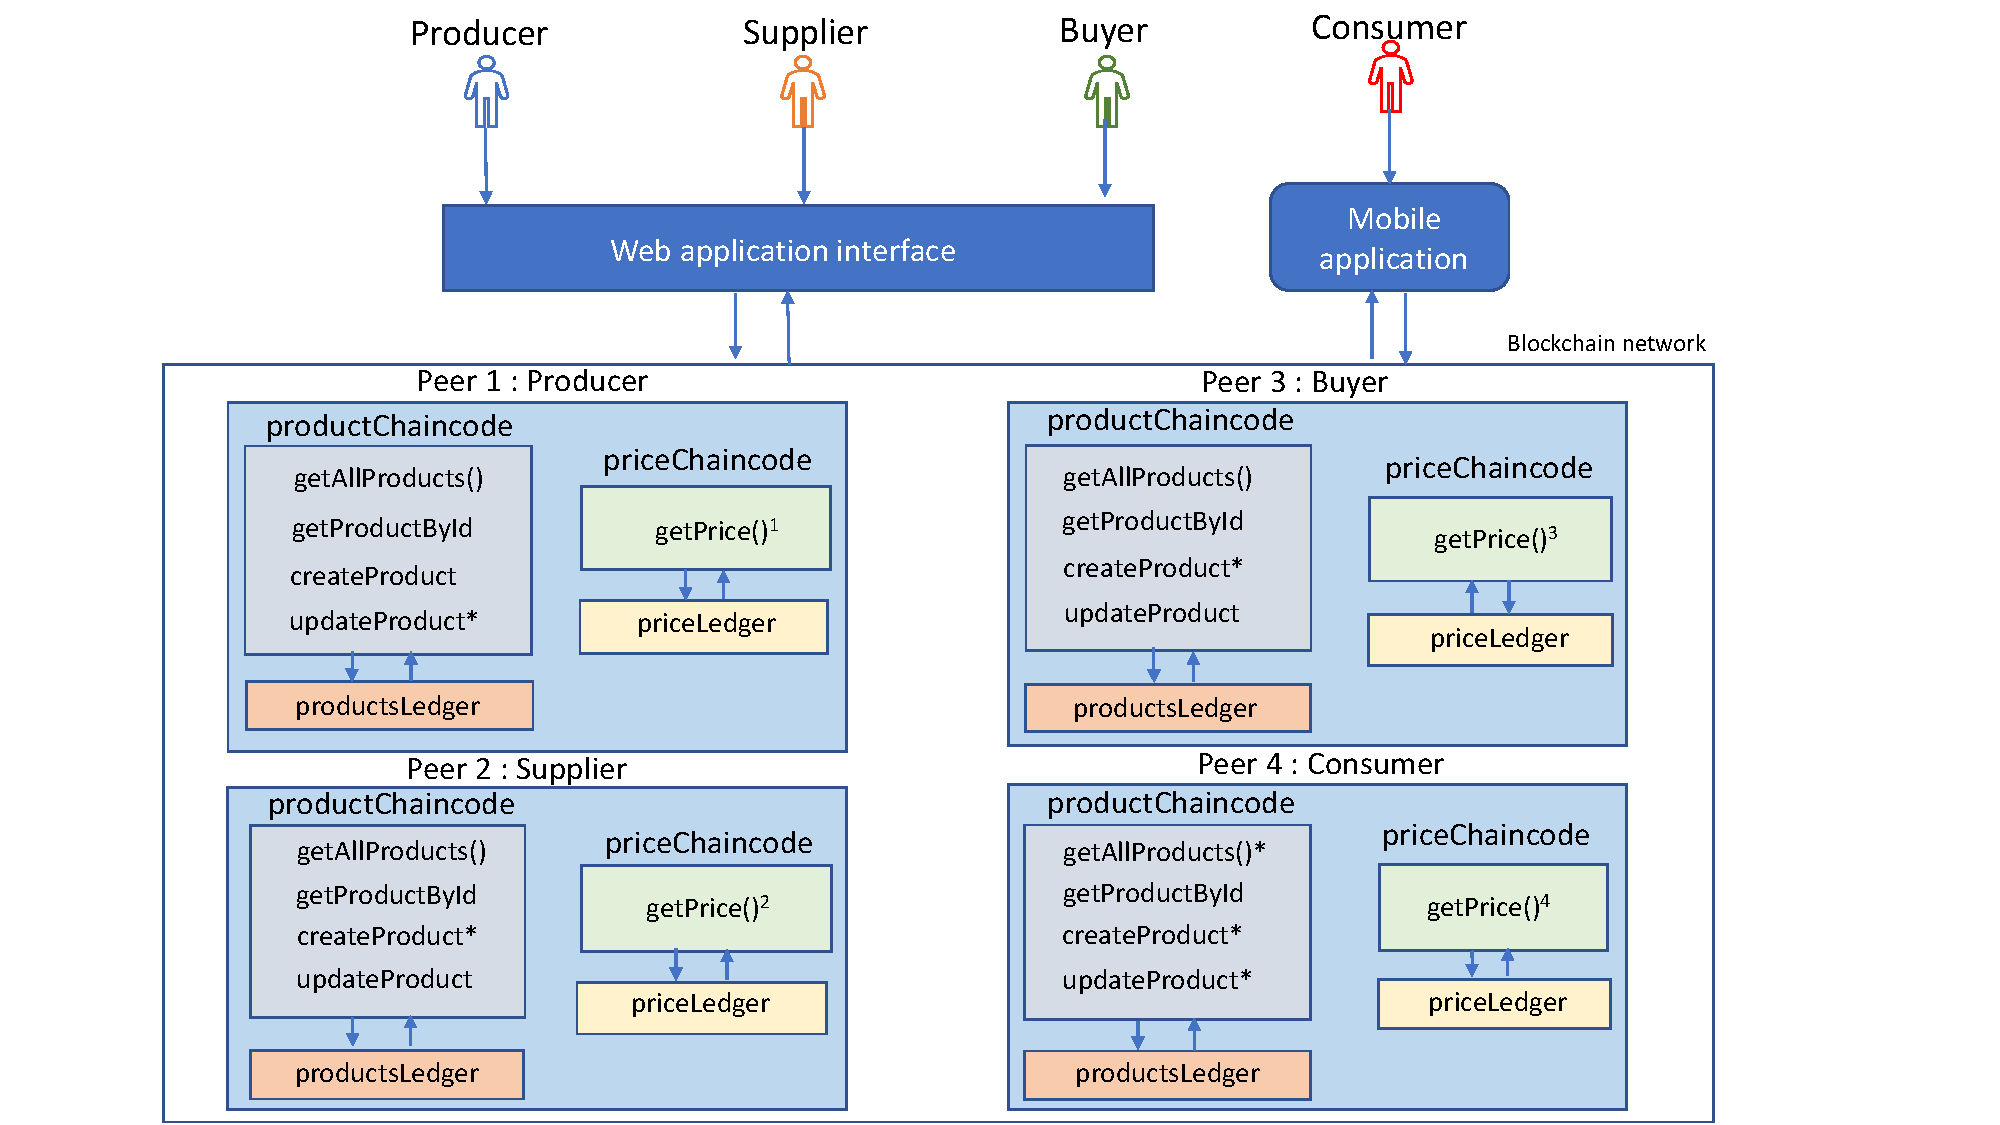
\includegraphics[width=20cm,height=20cm,keepaspectratio]{architecture.pdf}
\caption{Figure showing the architecture of the developed application. Methods marked with (*) will not be accessible to the corresponding users. The method  $getPrice()\textsuperscript{1}$ will fetch price for channel between Producer and Supplier, $getPrice()\textsuperscript{3}$ will fetch price for channel betwwen Supplier and Buyer, $getPrice()\textsuperscript{2}$ will fetch prices for both the channels, $getPrice()\textsuperscript{4}$ will fetch price for channel between buyer and consumer}.
\label{fig:arch}

\end{figure}

\section{System Architecture}
The participants of a blockchain network will be accessing the blockchain network from a web application interface and a mobile application. As shown in Figure \ref{fig:arch}, the different peers are associated with different participants of the network. This ensures that only the authorized peers can access the functions of the chaincode and can submit transaction on the blockchain network. Initially for the application, we created a single channel where all the participants are included in the channel and the use case is further extended with the experimentation in the next chapter where we use multiple channels. 

Depending upon the login credentials, the user identity is mapped to the login details and the peer and the view related to the user's permissions is shown on the screen. For example, the user \textbf{producer} will have access to three functions that include getting all the products details, get product detail by id and create a new product. The view for \textbf{producer} will only show these functions and it will be handled programatically. Additionally, there is an android application created that can be used to get a product by id, get a product by scanning QR-Code. Also the app can be used by different users like \textbf{producer}, \textbf{supplier}, \textbf{buyer} to perform the associated functions.

As it is seen in Figure \ref{fig:arch}, the peer for the \textbf{producer} will have two chaincodes installed on it. The \textbf{productChaincode} contains all the functions related to the products like querying, updating and creating a new product. However, the producer has no access to the \textbf{updateProduct} method of the chaincode. Similarly, supplier and buyer has no access to \textbf{createProduct}, consumer has no access to \textbf{getAllProducts}, \textbf{createProduct} and \textbf{updateProduct}. The chaincodes maintain their own state and the \textbf{priceChaincode} will have its own state containing price information. Both the chaincodes maintain their separate ledger that is distributed over the network. 

There are three \footnote{the fourth channel for price between buyer and consumer is not created} different channels created in the application, one channel between the producer and supplier for the agreed price, one channel between the supplier and buyer for the agreed price and one channel for the product functions. In short there are two channels for price and one channel for the product processing functions.  


\section{User Roles}
The blockchain application will have four different type of participants with each participant having its own functions in the blockchain application. Figure \ref{fig:actors} shows the different actors in the developed blockchain application. The description of the participants is as follows:
\begin{figure}[h!]
\begin{center}
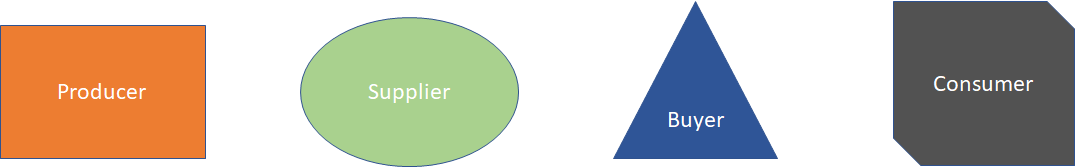
\includegraphics[width=\textwidth]{actors.png}
\caption{Figure showing different participants in the blockchain application.}
\label{fig:actors}
\end{center}
\end{figure}

\begin{figure}[b!]
\begin{center}
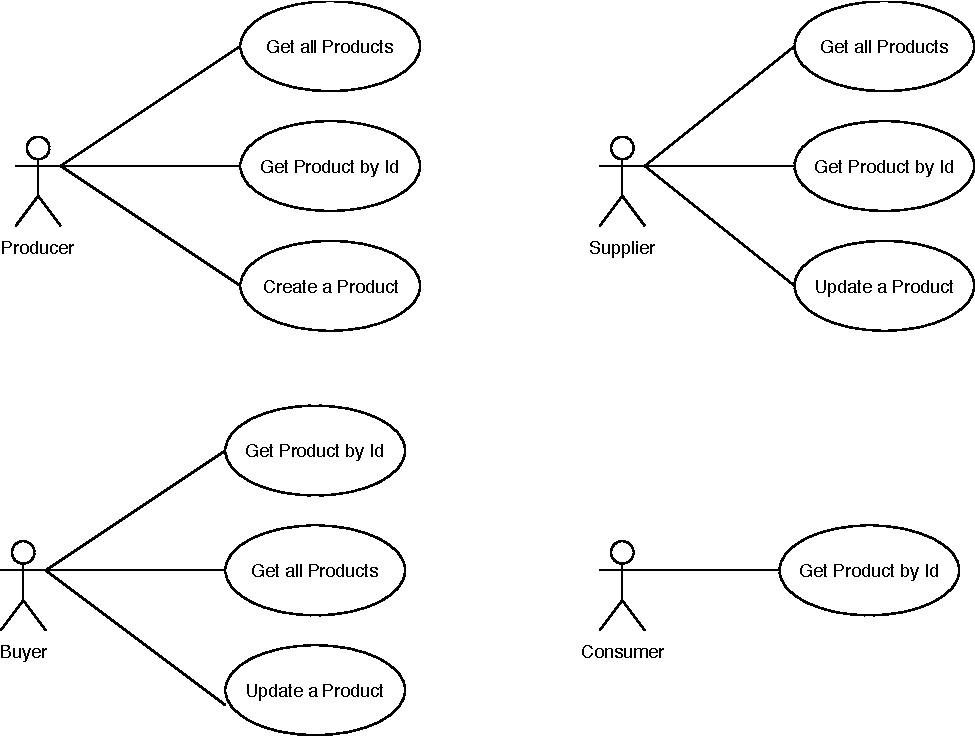
\includegraphics[width=\textwidth]{uml.pdf}
\caption{Use case diagram for the different participants. The first figure shows the use case diagram for producer, second figure shows the use case diagram for supplier, third figure for the buyer and fourth figure for the consumer.}
\label{fig:uml}
\end{center}
\end{figure}

\begin{itemize}
    \item \textbf{Producer}: The producer of product can be any manufacturer that creates products from finished goods. For example, a farmer who produces wheat in the field or a company that manufactures biscuits. The different functions associated with the producer are as follows:
    \begin{enumerate}
        \item \textbf{getAllProduct()}: Fetches the details about all the products.
        \item \textbf{getProductById()}: Fetches the details of a specific product identified by its id.
        \item \textbf{createProduct()}: Creates a new product with all the necessary and required fields.
    \end{enumerate}
    \item \textbf{Supplier}: The supplier is the link between the producer and buyer and plays an important role in the supply chain application. The supplier can be an organization or a company that delivers raw or finished goods to a buyer. The different functions associated with the supplier are as follows:
    \begin{enumerate}
        \item \textbf{getAllProduct()}: Fetches the details about all the products.
        \item \textbf{getProductById()}: Fetches the details of a specific product identified by its id.
        \item \textbf{updateProduct()}: Updates the owner of the product as it moves in the supply chain.
    \end{enumerate}
    \item \textbf{Buyer}: A buyer is the one who gets the product produced by the producer and can further process it or sell it the way its delivered. The buyer can be a supermarket store, vehicle manufacturer or other such manufacturing units. The different functions associated with the buyer are as follows:
    \begin{enumerate}
        \item \textbf{getAllProduct()}: Fetches the details about all the products.
        \item \textbf{getProductById()}: Fetches the details of a specific product identified by its id.
        \item \textbf{updateProduct()}: Updates the owner of the product as it moves in the supply chain.
    \end{enumerate}
    \item \textbf{Consumer}: The consumer is the last point in the supply chain and is the one who enjoys the services of the final finished good after purchasing it from the manufacturer or from a supermarket. The different functions associated with the consumer are as follows:
    \begin{enumerate}
        \item \textbf{getProductById()}: Fetches the details about a particular product specified with the Id.
    \end{enumerate}
\end{itemize}



\section{Use Cases}
As discussed before, there are four different participants in the network where each participant has a specific set of functions. The use case diagram helps to understand the different functions \footnote{The function \textit{getPrice()} is associated with the Product and is called as a promise function after the product response in the corresponding channel} a participant can perform and the constraints and possible outcomes are also discussed. Figure \ref{fig:uml} shows the different participants in the network and their functions with the help of a use-case diagram.

The details about the different use-cases is described further: 


\begin{table}[h!]
\begin{center}
    \begin{tabular}{ | l | p{9cm} |}
    \hline
    \textbf{Name} & \textbf{Get all Products} \\ \hline
    Goal & Get all the details about all the products on the blockchain network. \\ \hline
    Actor & Producer, Supplier, Buyer \\ \hline
    Pre-condition & The logged user should have proper authorization to perform the function. \\ \hline
    Post-condition & The details about the product like owner, location, datetime and product Id are shown in a table. \\ \hline
    Post-condition in Special Case & The user is not authorized to perform the action and hence, no results are shown.\\ \hline
    Normal Case & \begin{itemize}
        \item The user clicks on the button that fetches all the products.
        \item A chaincode query is executed against the world state on the local peer and response is returned in a json format.
        \item The response from the blockchain is handled by the front-end application that parses the data and shows it in a tabular format.
    \end{itemize}\\ \hline
    Special Cases & Request to get the product details failed because the user now is no longer a part of the network or its membership has been revoked. \\ \hline
    \end{tabular}
\end{center}
\caption{Description for the use case \textit{Get all Products} for the participants \textit{Producer}, \textit{Supplier}, \textit{Buyer}.}
    \label{tab:uc1}
\end{table}

\begin{table}[t!]
\begin{center}
    \begin{tabular}{ | l | p{9cm} |}
    \hline
    \textbf{Name} & \textbf{Get Product by Id} \\ \hline
    Goal & Get all the details about a product by querying it with its Id on the blockchain network. \\ \hline
    Actor & Producer, Supplier, Buyer, Consumer \\ \hline
    Pre-condition & The logged user should have proper authorization to perform the function. \\ \hline
    Post-condition & The details about the product, specified with the Id, like owner, location, datetime and product Id are shown in a table. \\ \hline
    Post-condition in Special Case & \begin{itemize}
        \item The user is not authorized to perform the action and hence, no results are shown.
        \item The product with the specified Id does not exist in the blockchain network.
    \end{itemize}\\ \hline
    Normal Case & \begin{itemize}
        \item The user enter the Product Id and clicks on the button that the details about a specific product.
        \item A chaincode query is executed against the world state on the local peer and response is returned in a json format.
        \item The response from the blockchain is handled by the front-end application that parses the data and shows it in a tabular format.
    \end{itemize}\\ \hline
    Special Cases & \begin{itemize}
        \item Request to get the product details failed because the user now is no longer a part of the network or its membership has been revoked.
        \item No response returned as the product with the specified Id is not there in the network.
    \end{itemize} \\ \hline
    \end{tabular}
\end{center}
\caption{Description for the use case \textit{Get Product by Id} for the participant \textit{Producer}, \textit{Buyer}, \textit{Supplier}, \textit{Consumer}.}
    \label{tab:uc2}
\end{table}

\begin{table}[t!]
\begin{center}
    \begin{tabular}{ | l | p{9cm} |}
    \hline
    \textbf{Name} & \textbf{Create a Product} \\ \hline
    Goal & Create a new product in the blockchain network by providing all the details. \\ \hline
    Actor & Producer \\ \hline
    Pre-condition & The logged user should have proper authorization to perform the function. \\ \hline
    Post-condition & A new product with the supplied values for owner, location, datetime and product Id fields is created. \\ \hline
    Post-condition in Special Case & The user is not authorized to perform the action and hence, transaction fails.\\ \hline
    Normal Case & \begin{itemize}
        \item The user enter product Id, owner, location, datetime for the product.
        \item A chaincode invoke transaction is executed on the peer and the results after validation are submitted to all the peers and transaction is committed.
        \item The response from the blockchain contains the transaction Id of the transaction and it is displayed on the web and mobile application.
    \end{itemize} \\ \hline
    Special Cases & \begin{itemize}
        \item Request to get the product details failed because the user now is no longer a part of the network or its membership has been revoked.
        \item The ordering service is down and as a result the transaction cannot be put in blocks and cannot be committed. Transactions failure notification is shown in the application.
    \end{itemize}\\ \hline
    \end{tabular}
\end{center}
\caption{Description for the use case \textit{Create a Product} for the participant \textit{Producer}.}
    \label{tab:uc3}
\end{table}

\begin{table}[t!]
\begin{center}
    \begin{tabular}{ | l | p{9cm} |}
    \hline
    \textbf{Name} & \textbf{Update a Product} \\ \hline
    Goal & Update the \textbf{Owner} field of the product as it flows through the supply chain. \\ \hline
    Actor & Supplier, Buyer \\ \hline
    Pre-condition & The logged user should have proper authorization to perform the function. \\ \hline
    Post-condition & The product is updated with the new owner and result can be verified by quering. \\ \hline
    Post-condition in Special Case & \begin{itemize}
        \item The user is not authorized to perform the action and hence, transaction fails.
        \item The Product with specified Id does not exist resulting in error.
    \end{itemize}\\ \hline
    Normal Case & \begin{itemize}
        \item The user enter the Product Id and owner for which the update is required.
        \item A chaincode invoke transaction is executed on the peer and the transaction is sent to the ordering service. The ordering service puts the transaction in a block and broadcasts it to all peers that eventually commit it.
        \item The response contains the transaction Id of the invoke transaction and acknowledgement about transaction status that is shown in the application.
    \end{itemize}\\ \hline
    Special Cases & \begin{itemize}
        \item Request to get the product details failed because the user now is no longer a part of the network or its membership has been revoked.
        \item The ordering service is down and as a result the transaction cannot be put in blocks and cannot be committed. Transactions failure notification is shown in the application.
    \end{itemize}\\ \hline
    \end{tabular}
\end{center}
\caption{Description for the use case \textit{Update a Product} for the participant \textit{Buyer}, \textit{Supplier}.}
    \label{tab:uc4}
\end{table}
\clearpage
\section{Data Model}
The data model defines the schema of the data that is going to be used in the application. The product has information like \textbf{ProductId}, \textbf{Location}, \textbf{Owner}, \textbf{Datetime} which is maintained in a separate ledger called \textbf{productLedger} on every peer. Similarly, the Price schema defines the information required to get a product's price. It has fields like \textbf{ProductId} and \textbf{Price}. The Price schema is maintained by the priceLedger on every peer. Figure \ref{fig:dm} shows the data model for the application developed.
\begin{figure}[h!]
\begin{center}
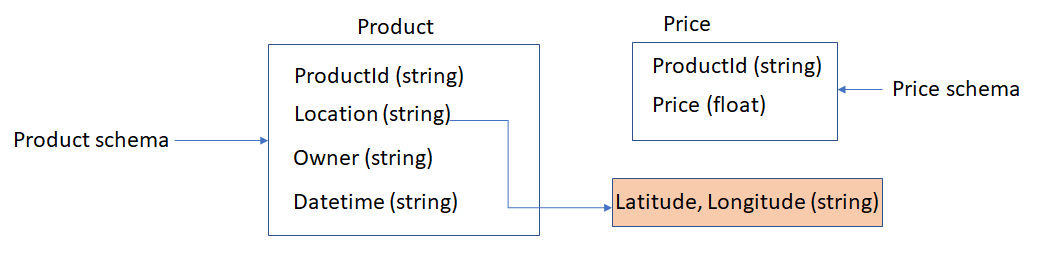
\includegraphics[width=\textwidth]{dataModel.png}
\caption{Figure showing the schema of product and price that are maintained in two different ledgers.}
\label{fig:dm}
\end{center}
\end{figure}
The importance of the various properties can be explained as:
\begin{enumerate}
    \item \textbf{ProductId}: Every product is unique and therefore, ProductId is the primary key for the product that can be used to query a product.
    \item \textbf{Location}: The Location property defines the current location of the product in the supply chain. The location field is composed of latitude and longitudes for exact geographical location.
    \item \textbf{Owner}: The Owner fields defines the current owner of the product in the supply chain. This helps to understand the flow of product through different people and can be used for traceability and quality analysis.
    \item \textbf{Datetime}: This field defines the processing time of the product at that specific location with the owner mentioned in the Owner field.
    \item \textbf{Price}: This field shows the price of the product. The Price is fetched from different channels and one product may have different prices as it is on different channels.
\end{enumerate}
All these properties help in properly understanding the flow of products in supply chain as the product moves and reaches to the end user. It helps in traceability, quality analysis, dispute resolution and creation of trust environment between the participants.

\section{Chaincode functions}
Chaincode contain the actual business logic for the blockchain network. It deals with the transaction execution on the peer on which it is attached and the results are then sent to all the peer for committing so that every peer maintains a shared copy of the same data. There are two types of chaincode methods:
\begin{itemize}
    \item \textbf{Init} method: The Init method is called whenever the chaincode is instantiated or upgraded on a channel \cite{Chaincode}. The initialization is accompanied with initialization of the world state by creating keys and their corresponding values.
    \item \textbf{Invoke} method: The Invoke method is called whenever an invoke transaction is explicitly specified on the peer. In other words, Invoke method creates a transaction proposal on the peer on which it is executed.
\end{itemize}
Let us examine the different chaincode methods \cite{cm} developed in the application.

\begin{Listing}[b!]
\begin{lstlisting}
// product-chaincode.go
/*
 This code is based on code written by the Hyperledger Fabric community.
 Original code can be found here: https://github.com/hyperledger/fabric-samples/blob/release/chaincode/fabcar/fabcar.go
*/

/*
 * The Invoke method *
 called when an application requests to run the chaincode "product-chaincode"
 The app also specifies the specific chaincode function to call with args
*/
func (s *SmartContract) Invoke(APIstub shim.ChaincodeStubInterface) sc.Response {

	// Retrieve the requested chaincode function and arguments
	function, args := APIstub.GetFunctionAndParameters()
	// Route to the appropriate handler function to interact with the ledger
	if function == "queryProduct" {
		return s.queryProduct(APIstub, args)
	} else if function == "initLedger" {
		return s.initLedger(APIstub)
	} else if function == "createProduct" {
		return s.createProduct(APIstub, args)
	} else if function == "queryAllProducts" {
		return s.queryAllProducts(APIstub)
	} else if function == "changeProductOwner" {
		return s.changeProductOwner(APIstub, args)
	}

	return shim.Error("Invalid chaincode function name.")
}
\end{lstlisting}
\caption{Code snippet for the Invoke method in the product-chaincode.go}
\label{lst:invoke}
\end{Listing}

%Listing \ref{lst:invoke} shows the Invoke method of the product-chaincode file. The peer can call this method on the installed chaincode\footnote{For a peer to invoke any method the chaincode must be installed on that peer.} and can specify which function has to be called with the required parameters in \textbf{Args} parameter specified in the cli command.

\begin{Listing}[h!]
\begin{lstlisting}
/*
 * The queryProduct method *
Used to view the records of one particular product
It takes one argument -- the productId for the product to be searched
*/
func (s *SmartContract) queryProduct(APIstub shim.ChaincodeStubInterface, args []string) sc.Response {

	if len(args) != 1 {
		return shim.Error("Incorrect number of arguments. Expecting 1")
	}

	productAsBytes, _ := APIstub.GetState(args[0])
	if productAsBytes == nil {
		return shim.Error("Could not locate product")
	}
	return shim.Success(productAsBytes)
}
\end{lstlisting}
\caption{Code snippet for the \textit{queryProduct} method in the product-chaincode.go}
\label{lst:queryPId}
\end{Listing}
%Listing \ref{lst:queryPId} shows the chaincode function that fetches a product based upon the product Id entered by the user. The function requires a parameter for the key that it searches in the world state and returns the latest value.
\begin{Listing}[h!]
\begin{lstlisting}
/*
 * The createProduct method *
This method will be used by the Producer to create a record of a new product that becomes part of the supply chain.
*/
func (s *SmartContract) createProduct(APIstub shim.ChaincodeStubInterface, args []string) sc.Response {

	if len(args) != 5 {
		return shim.Error("Incorrect number of arguments. Expecting 5")
	}

	var product = Product{Price: args[1], Location: args[2], Timestamp: args[3], Owner: args[4]}

	productAsBytes, _ := json.Marshal(product)
	err := APIstub.PutState(args[0], productAsBytes)
	if err != nil {
		return shim.Error(fmt.Sprintf("Failed to record product: %s", args[0]))
	}

	return shim.Success(nil)
}
\end{lstlisting}
\caption{Code snippet for the \textit{createProduct} method in the product-chaincode.go}
\label{lst:create}
\end{Listing}

\begin{Listing}[h!]
\begin{lstlisting}
/*
 * The queryAllProducts method *
allows for assessing all the records added to the ledger(all the products in the ledger)
This method will return an array of JSON response that can be parsed by the front-end applications to show the results.
*/
func (s *SmartContract) queryAllProducts(APIstub shim.ChaincodeStubInterface) sc.Response {

	startKey := "0"
	endKey := "999"

	resultsIterator, err := APIstub.GetStateByRange(startKey, endKey)
	if err != nil {
		return shim.Error(err.Error())
	}
	defer resultsIterator.Close()

	// buffer is a JSON array containing QueryResults
	var buffer bytes.Buffer
	buffer.WriteString("[")

	bArrayMemberAlreadyWritten := false
	for resultsIterator.HasNext() {
		queryResponse, err := resultsIterator.Next()
		if err != nil {
			return shim.Error(err.Error())
		}
		// Add comma before array members,suppress it for the first array member
		if bArrayMemberAlreadyWritten == true {
			buffer.WriteString(",")
		}
		buffer.WriteString("{\"Key\":")
		buffer.WriteString("\"")
		buffer.WriteString(queryResponse.Key)
		buffer.WriteString("\"")

		buffer.WriteString(", \"Record\":")
		// Record is a JSON object, so we write as-is
		buffer.WriteString(string(queryResponse.Value))
		buffer.WriteString("}")
		bArrayMemberAlreadyWritten = true
	}
	buffer.WriteString("]")

	fmt.Printf("- queryAllProducts:\n%s\n", buffer.String())

	return shim.Success(buffer.Bytes())
}
\end{lstlisting}
\caption{Code snippet for the \textit{queryAllProducts} method in the product-chaincode.go}
\label{lst:query}
\end{Listing}

\begin{Listing}[h!]
\begin{lstlisting}
/*
 * The changeProductOwner method *
The data in the world state can be updated with currently has the product.
This function takes in 2 arguments, product id and new owner name.
*/
func (s *SmartContract) changeProductOwner(APIstub shim.ChaincodeStubInterface, args []string) sc.Response {

	if len(args) != 2 {
		return shim.Error("Incorrect number of arguments. Expecting 2")
	}

	productAsBytes, _ := APIstub.GetState(args[0])
	if productAsBytes == nil {
		return shim.Error("Could not locate product")
	}
	product := Product{}

	json.Unmarshal(productAsBytes, &product)
	// Normally check that the specified argument is a valid owner of the product
	// we are skipping this check for this example
	product.Owner = args[1]

	productAsBytes, _ = json.Marshal(product)
	err := APIstub.PutState(args[0], productAsBytes)
	if err != nil {
		return shim.Error(fmt.Sprintf("Failed to change product owner: %s", args[0]))
	}

	return shim.Success(nil)
}
\end{lstlisting}
\caption{Code snippet for the \textit{changeProductOwner} method in the product-chaincode.go}
\label{lst:update}
\end{Listing}
\begin{Listing}[h!]
\begin{lstlisting}
/*
 * main function *
calls the Start function
The main function starts the chaincode in the container during instantiation.
*/
func main() {

	// Create a new Smart Contract
	err := shim.Start(new(SmartContract))
	if err != nil {
		fmt.Printf("Error creating new Smart Contract: %s", err)
	}
}
\end{lstlisting}
\caption{Code snippet for the \textit{main} method in the product-chaincode.go}
\label{lst:main}
\end{Listing}

\section{Web front-end application}
In this section, we will see the structure and flow of different actions that a user can perform with the front-end application. The user is authenticated with the login credentials and depending upon the type of user, different actions are performed by the user. The application uses the Hyperledger Fabric Client SDK to interact with the blockchain ledger.

\subsection{Get All Products}
Here we will see the front-end application part where we get all the details about all the products. We will also see how the blockchain network chaincode function \textbf{queryAllProducts} is called from the front-end application.

\begin{figure}[h!]
\begin{center}
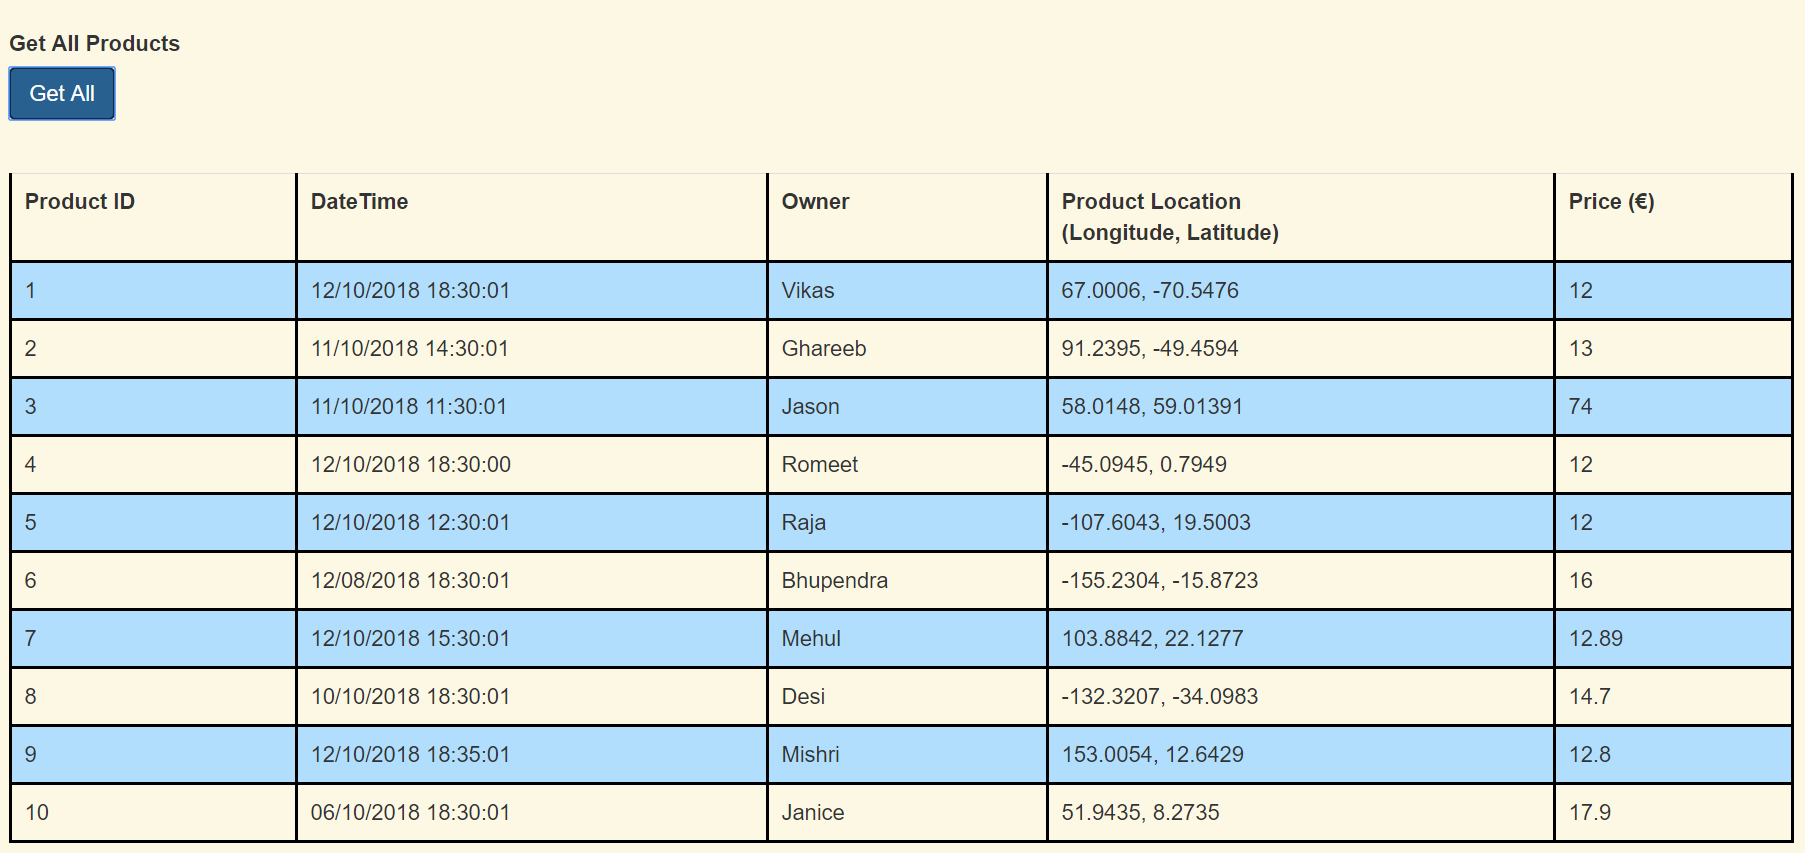
\includegraphics[width=\textwidth]{getp.png}
\caption{The view for displaying all the products in the blockchain.}
\label{fig:ga}
\end{center}
\end{figure}
Figure \ref{fig:ga} shows the product detail view as the product flows in the supply chain. The information about products get updated depending upon the user functions.
\begin{Listing}[h!]
\begin{lstlisting}
//define the object for the Fabric_Client SDK connection
var fabric_client = new Fabric_Client();

// setup the fabric network
//defines the name of the channel on which peer has to execute transaction
var channel = fabric_client.newChannel('mychannel');
//creates a peer object by passing its unique docker url
var peer = fabric_client.newPeer('grpc://192.168.99.100:7051');
//adds the peer object to the channel object for transaction execution
channel.addPeer(peer);
\end{lstlisting}
\caption{Code snippet for the connecting to the Fabric Client SDK.}
\label{lst:fc}
\end{Listing}
\begin{Listing}[h!]
\begin{lstlisting}
// queryAllProducts - requires no arguments , ex: args: [''],
    const request = {                 //request defines the request object created
    chaincodeId: 'product-chaincode', //the chaincode name on which transaction is executed
    txId: tx_id,                      //transaction id assigned to this action
    fcn: 'queryAllProducts',          //chaincode function name
    args: ['']                        //args represent the function parameters
};
\end{lstlisting}
\caption{Code snippet for the \textit{queryAllProducts} method in the controller function that calls the chaincode with the chaincodeId}
\label{lst:gapd}
\end{Listing}

\subsection{Get Product by Id}
This view represents the specific product that can be viewed by passing its product id. It requires one parameter, the name of the key which has to be searched in the world state. In our scenario, the key is the product id that was created by the user or during initialization.
\begin{figure}[h!]
\begin{center}
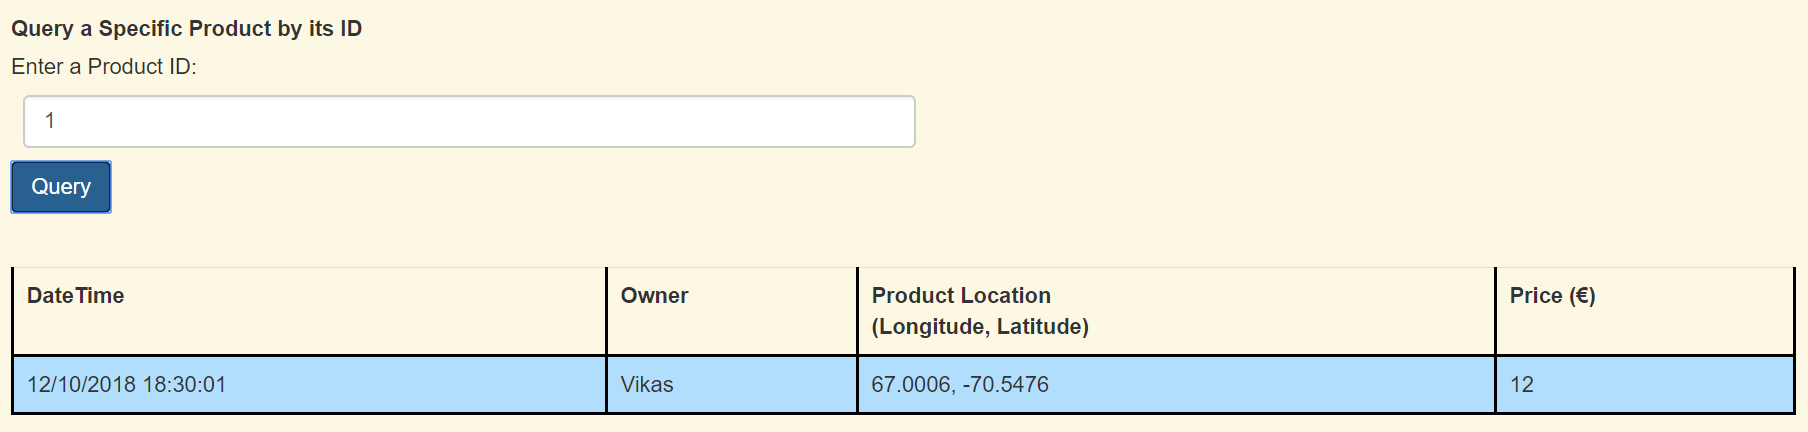
\includegraphics[width=\textwidth]{getPId.png}
\caption{The view for fetching a product by its id in the blockchain.}
\label{fig:gpi}
\end{center}
\end{figure}
\begin{Listing}[h!]
\begin{lstlisting}
// queryProduct - requires 1 argument, ex: args: ['4'],
    //the request object created to pass to the client SDK
    const request = { 
    //name of the installed chaincode for transaction execution
    chaincodeId: 'product-chaincode', 
    //the generated transaction id
    txId: tx_id,
    //name of the method in the chaincode
    fcn: 'queryProduct',
    //the value of the id passed to the controller
    args: [id]                    
};
\end{lstlisting}
\caption{Code snippet for the \textit{queryProduct} method in the controller function that calls the chaincode with the chaincodeId}
\label{lst:gapi}
\end{Listing}

\subsection{Create a Product}
Here we will see the view designed for creating a new product in the blockchain network. The producer has the permissions to create a new product that becomes part of the supply chain.
\begin{figure}[h!]
\begin{center}
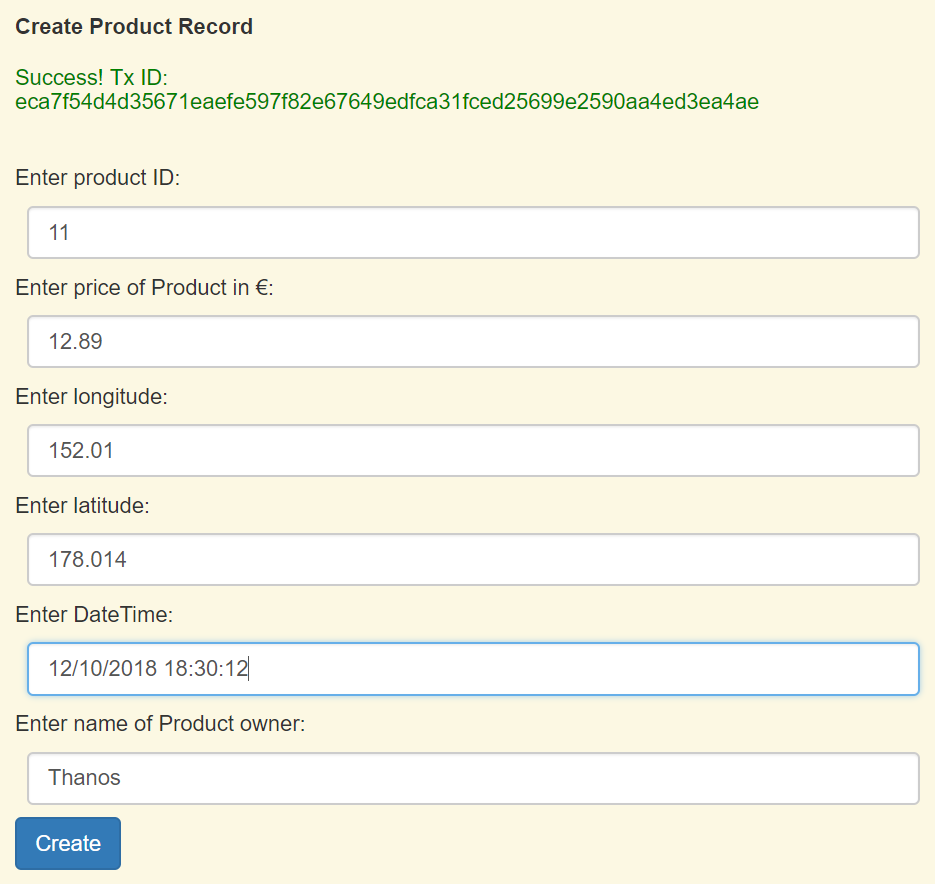
\includegraphics[width=\textwidth, height=9cm, keepaspectratio]{graphics/createProductSuccess.png}
\caption{The view for creating a new product and the acknowledgement of the transaction with transaction id}
\label{fig:cp}
\end{center}
\end{figure}
\begin{Listing}[h!]
\begin{lstlisting}
 // the request object is sent to the endorser as a proposal
    const request = {
    //name of the installed chaincode for transaction execution
    chaincodeId: 'product-chaincode',
    //name of the method in the chaincode
    fcn: 'createProduct',
    //the required fields passed to the controller
    args: [id, price, location, timestamp, owner],
    //name of the channel
    chainId: 'mychannel',
    //the generated transaction id
    txId: tx_id
};

// after the request is created, the transaction proposal is sent to the peers
\end{lstlisting}
\caption{Code snippet for the \textit{createProduct} method in the controller function that calls the chaincode with the chaincodeId}
\label{lst:cpr}
\end{Listing}

\subsection{Update a Product}
As the product flows in the supply chain, it constantly changes hands. It is therefore, essential to update the recent owner of a product so that any future issues can be easily resolved. The Supplier and Buyer are the one who are between the Consumer and Producer. The product is updated whenever it flows from one user to the other.
\begin{figure}[h!]
\begin{center}
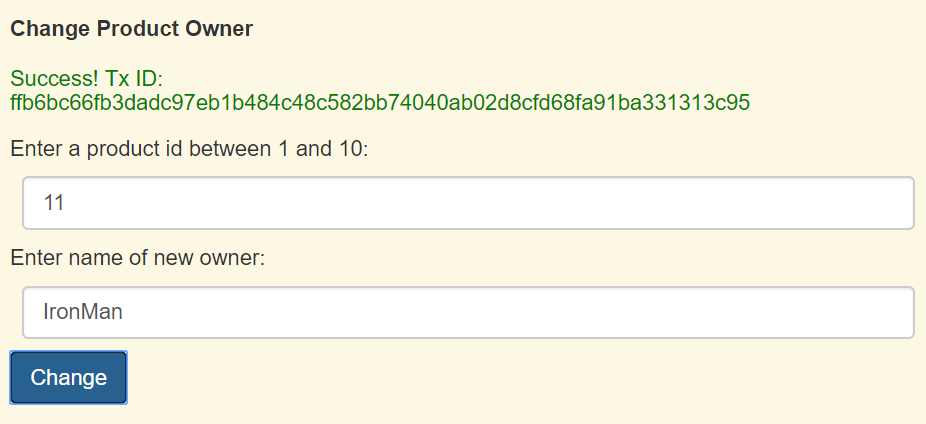
\includegraphics[width=\textwidth]{graphics/updateProductSuccess.png}
\caption{The view for updating a product with the new owner.}
\label{fig:up}
\end{center}
\end{figure}
\begin{Listing}[h!]
\begin{lstlisting}
 // the transaction proposal is created here and sent to endorser
    var request = {
    //name of the installed chaincode for transaction execution
    chaincodeId: 'product-chaincode',
    //name of the method in the chaincode
    fcn: 'changeProductOwner',
    //the required fields passed to the controller
    args: [id, owner],
    //name of the channel
    chainId: 'mychannel',
    //the transaction id generated in the request
    txId: tx_id
};

// after the request is created, the transaction proposal is sent to the peers
\end{lstlisting}
\caption{Code snippet for the \textit{changeProductOwner} method in the controller function that calls the chaincode with the chaincodeId}
\label{lst:upr}
\end{Listing}

\section{Android application}
The Android application is designed keeping the \textbf{Consumer} in mind. The consumer has no direct access to the web application. Thus, in order to check if a product has gone through all the required tests or to check if the product is illegitimate, the Consumer can use the app, scan the QR-Code on the product and verify the product details.
\begin{figure}[h!]
\begin{center}
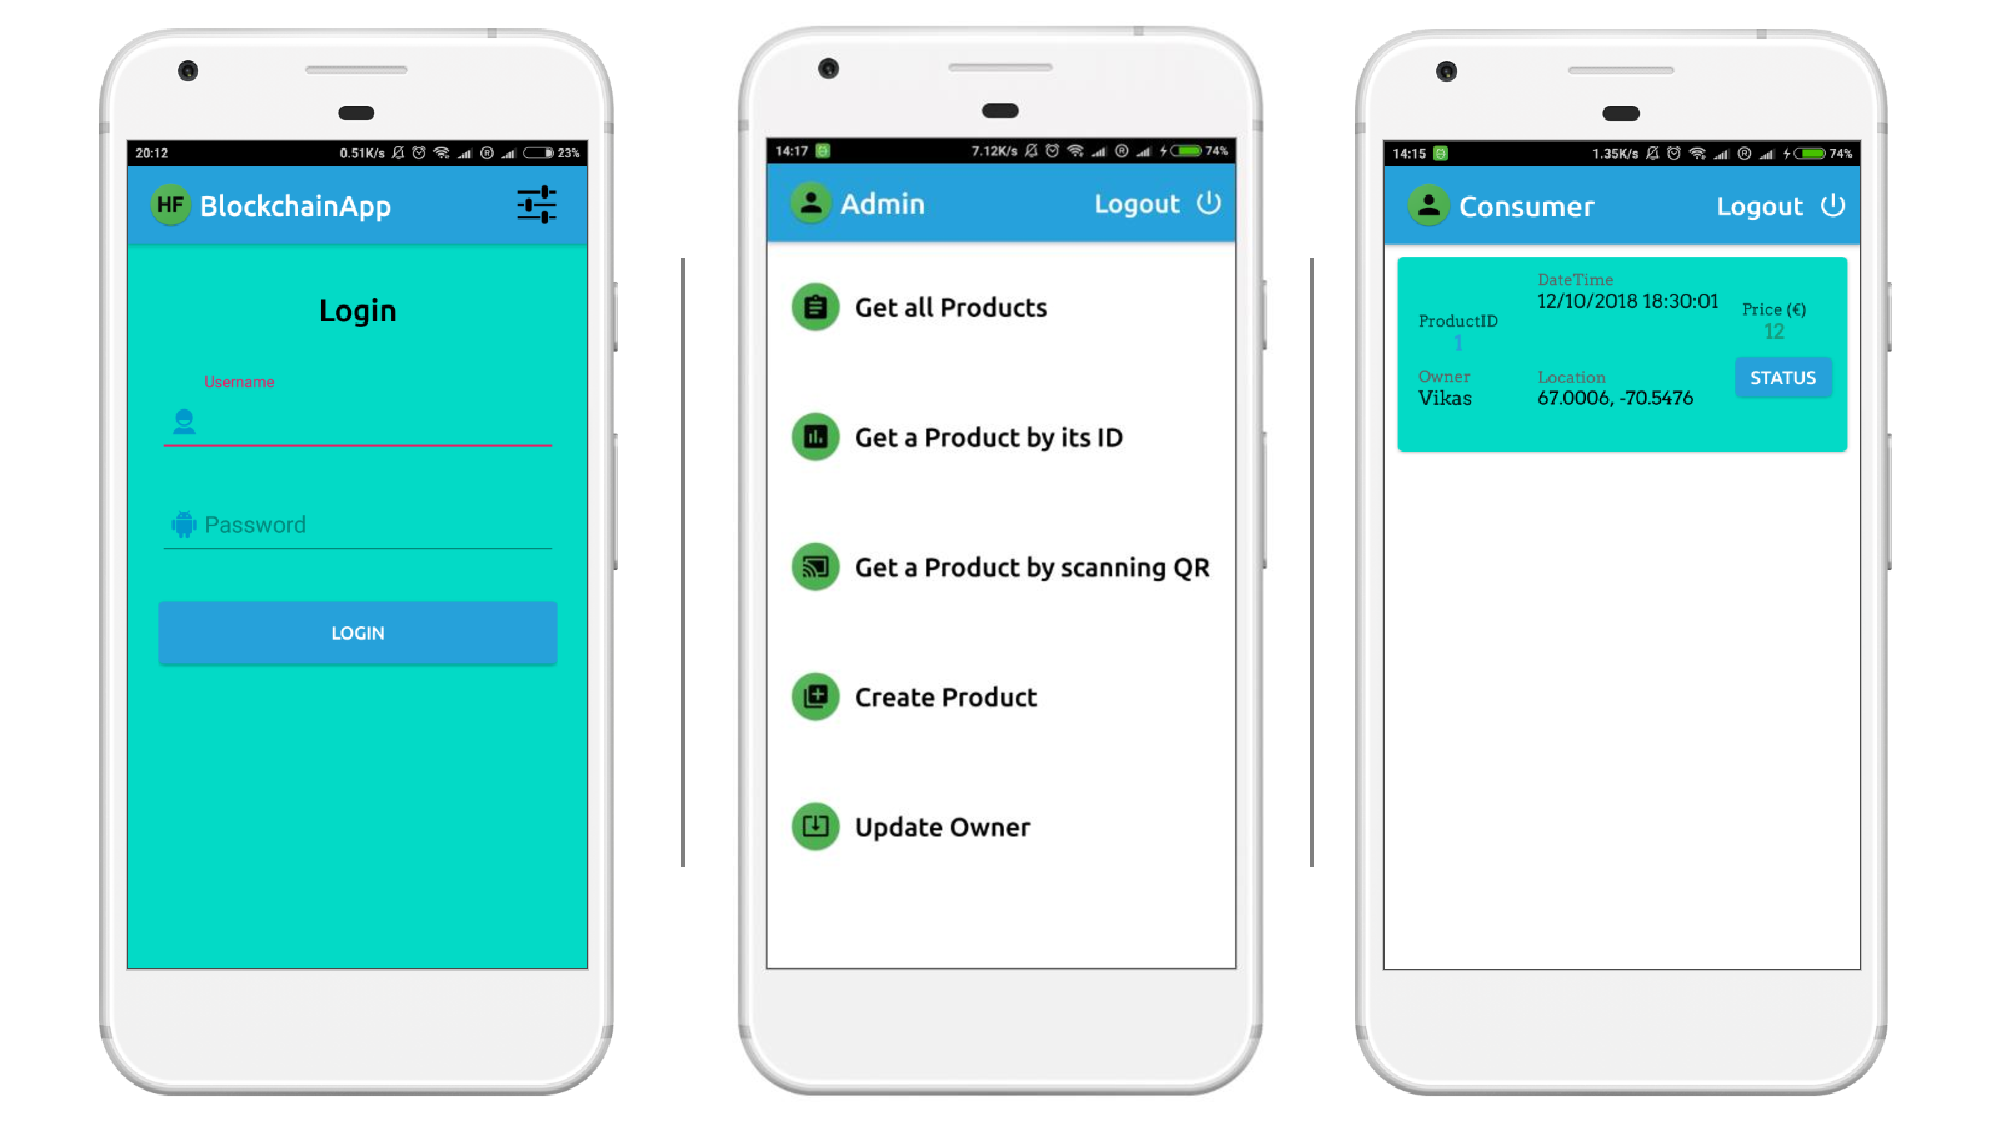
\includegraphics[width=\textwidth]{graphics/app1.pdf}
\caption{The mobile app screens designed for the blockchain network}
\label{fig:app1}
\end{center}
\end{figure}

Figure \ref{fig:app1} shows the different screens designed for the Android app. Authentication is required for the user to login to the blockchain network and to use the app. With the correct credentials, the view with the designated functions is shown to the user. For example, \textbf{Admin} user sees all the functions in the app. The \textbf{Consumer} can see the two relevant functions like \textit{Get a Product by its ID}, where the numeric id can be entered on the screen by the consumer, and \textit{Get a Product by scanning QR} where a QR can be scanned for the Product ID and the result will be shown as displayed in the third screen.

The app also works in the same way as the front-end web application works. The app is designed in JAVA using the Android SDK and is compatible with the Android devices running Android 3.0 or higher. 

Figure \ref{fig:arch2} shows the architecture of the app that uses the backend developed in Node.js. The request proposal is sent to the backend which then forwards it to the respective chaincode method. The chaincode method is executed on the peer and the transaction proposal response is sent back to the Node.js backend. The response is returned as a JSON response to the app which then parses the object and shows the result back to the user. The use cases in the app are similar to the web frontend application with additional feature of QR scanning for the product id.
\begin{figure}[h!]
\begin{center}
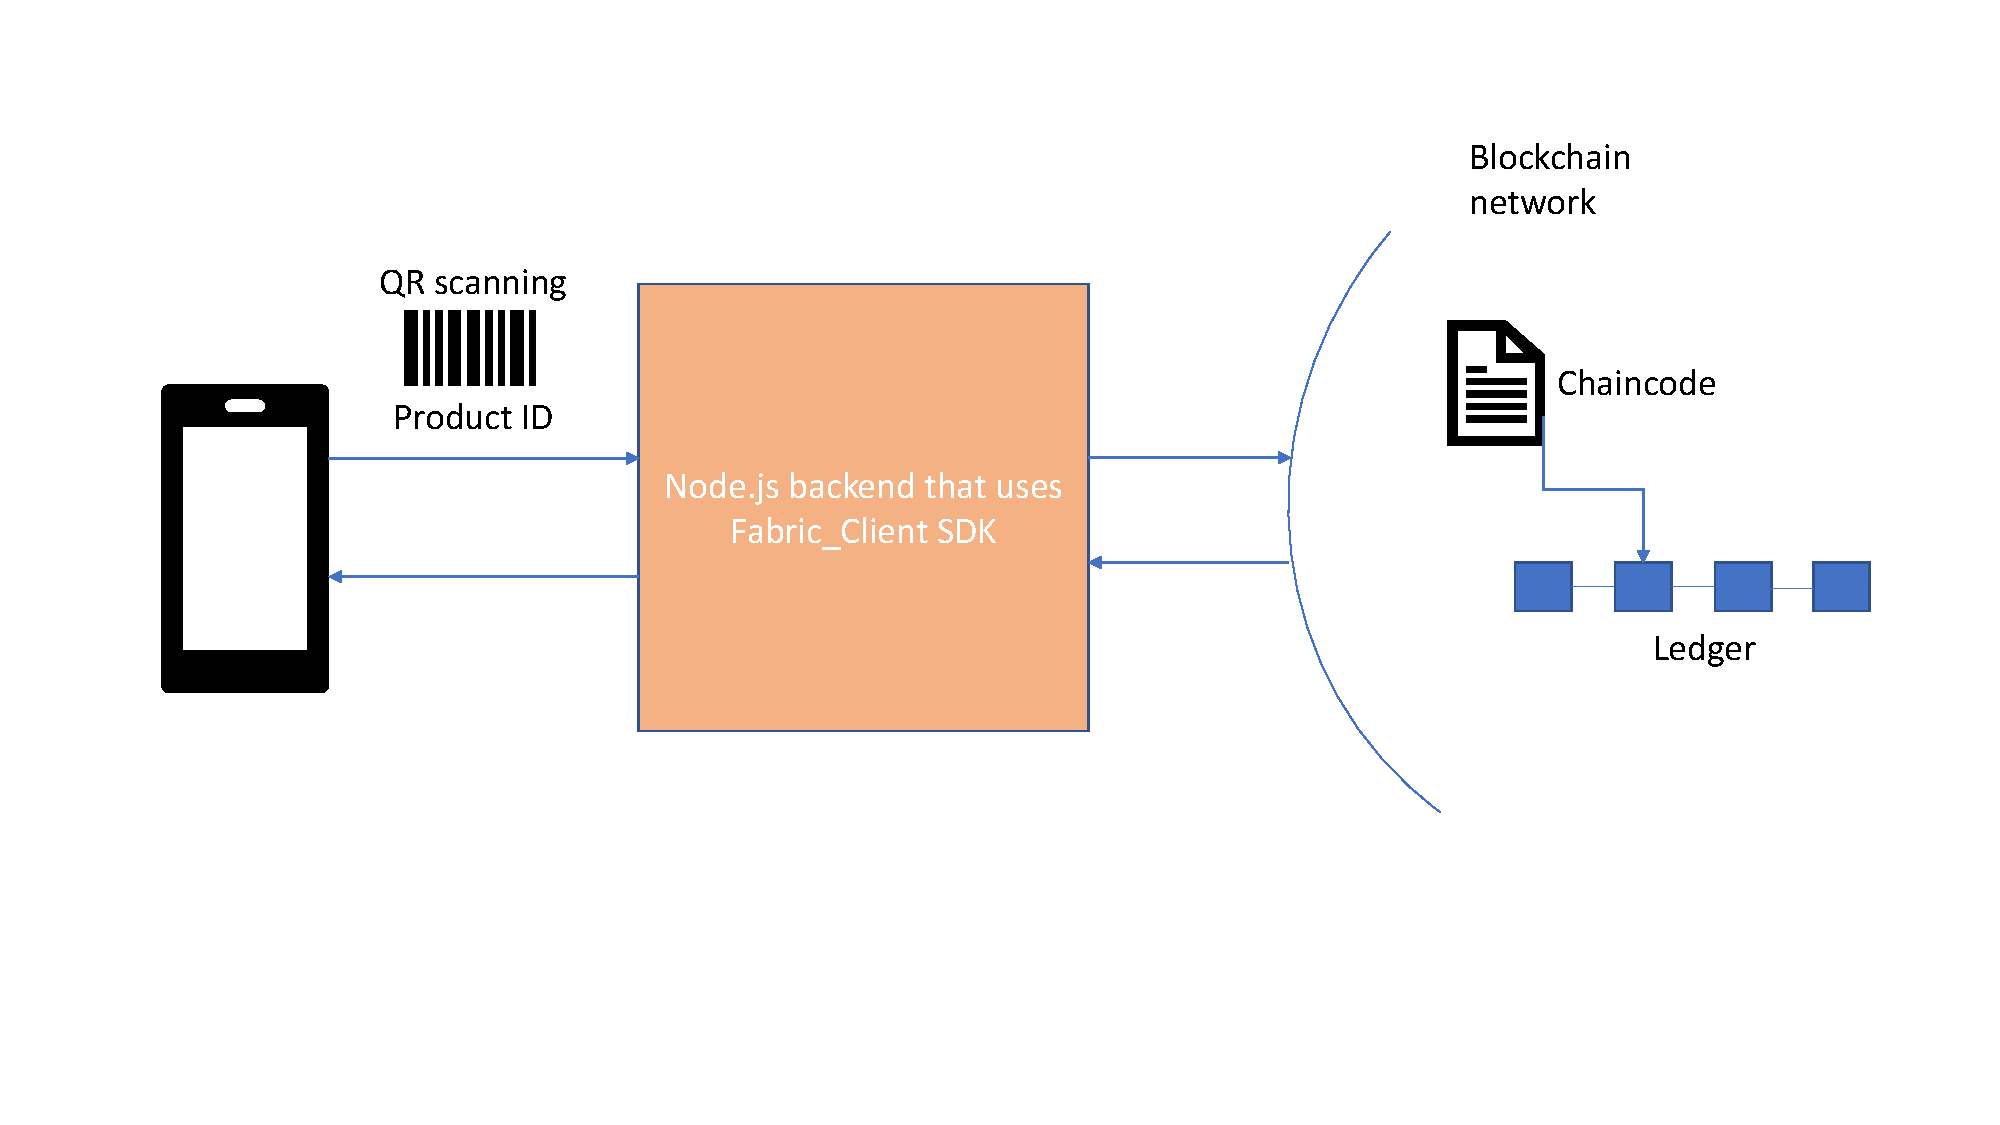
\includegraphics[width=\textwidth]{graphics/arch2.pdf}
\caption{The architecture of the mobile application interacting with the blockchain network.}
\label{fig:arch2}
\end{center}
\end{figure}

Figure \ref{fig:app2} shows the extension of the mobile application that can be designed to provide the important functionality of traceability and quality assurance. The extension is not discussed here and just shows the idea but can be implemented as a future work for the app.
\begin{figure}[h!]
\begin{center}
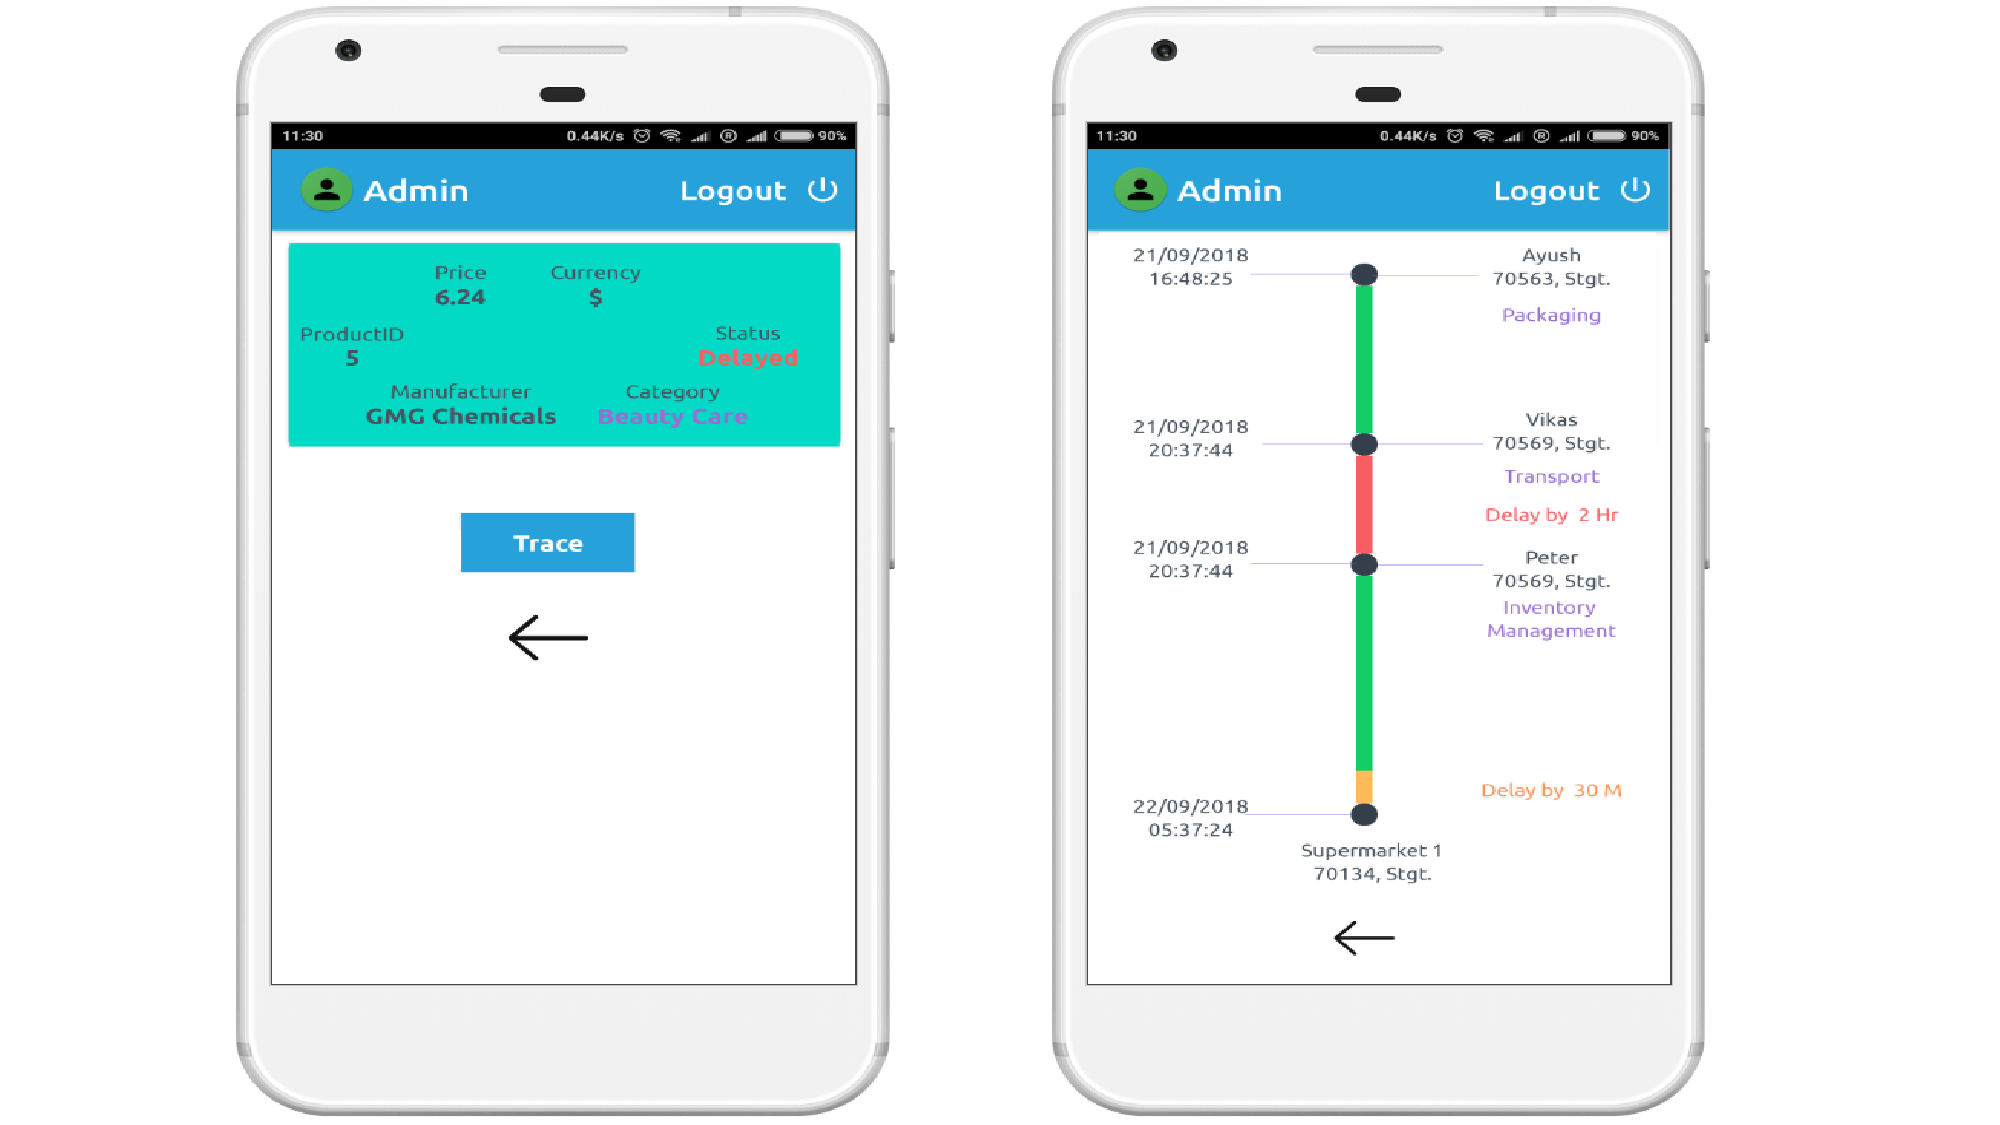
\includegraphics[width=\textwidth]{graphics/app2.pdf}
\caption{The extension of the app that can be used to view the status and other information about a product.}
\label{fig:app2}
\end{center}
\end{figure}

\chapter{Experimental Design and Results}
In this chapter, we will discuss the different experiments performed with the blockchain network to study various important transaction characteristics of permissioned blockchain networks. The business logic is written on the chaincode and therefore, the focus will be on chaincodes and the ledger for the experiments. 
\label{chap:de}

\section{Experiment 1: Chaincode to chaincode call on same channel}
\label{sec:exp1}
In this section we will see how a chaincode transaction is scoped when one chaincode calls another chaincode on the same channel. The chaincode call can be a read transaction on the world state or a write transaction on the world state and the blockchain. Therefore, the experiment will be divided into two subsections for read and write. We will verify and put forward the results.

\subsection{Read from same channel}
\label{sec:read}
There are various business transactions that require data from different applications in the network. Chaincodes contain the business logic for the blockchain applications and transactions can only be executed with the chaincodes method on the ledger. It is therefore important to study the behaviour of chaincode in a read operation requiring data from a different chaincode. 
\subsubsection{Experimental setup}
In this approach, we will use two different chaincodes, \textit{chaincode1} and \textit{chaincode2}. These chaincodes will be installed on the peer (considering a single peer) and will be on the same channel. In this setup, we will use chaincode2 methods to call chaincode1 method to read the world state. 

We will first create two keys \textbf{a} and \textbf{b} with some initial value by instantiating the chaincode chaincode1. Then we will instantiate chaincode2 with a key \textbf{sum} and initial value as \textbf{0}. Then with the help of chaincode2, we will call a method that reads the values of \textbf{a} and \textbf{b} and puts the values in the key \textbf{sum} that is scoped to chaincode2. The chaincode1 is based on the code at \cite{ce2} and chaincode2 at \cite{ce5}. 

Listing \ref{lst:c1i} shows the \textit{invoke} method defined in chaincode1 that deducts value from key \textbf{a} and adds the same value to key \textbf{b}.

Similarly, Listing \ref{lst:c2i} shows the invoke method for the chaincode2 that reads the keys \textbf{a} and \textbf{b} from chaincode1 and shows its sum in the key \textbf{sum} of chaincode2.
\begin{Listing}[h!]
\begin{lstlisting}
/* the experiment is based on the code at https://github.com/hyperledger/fabric/blob/release-1.3/examples/chaincode/go/example02/chaincode.go */
// Transaction makes payment of X units from A to B
func (t *SimpleChaincode) invoke(stub shim.ChaincodeStubInterface, args []string) pb.Response {
	
    //A and B are the arguments or keys initialized
	A = args[0]
	B = args[1]

	// Get the state from the ledger
	Avalbytes, err := stub.GetState(A)
	if err != nil {
		return shim.Error("Failed to get state")
	}
	Aval, _ = strconv.Atoi(string(Avalbytes))

	Bvalbytes, err := stub.GetState(B)
	if err != nil {
		return shim.Error("Failed to get state")
	}
	Bval, _ = strconv.Atoi(string(Bvalbytes))

	// Perform the execution
	X, err = strconv.Atoi(args[2])
	if err != nil {
		return shim.Error("Invalid transaction amount, expecting a integer value")
	}
	//sends a value from A to B
	Aval = Aval - X
	Bval = Bval + X
	fmt.Printf("Aval = %d, Bval = %d\n", Aval, Bval)

	// Write the state back to the ledger
	err = stub.PutState(A, []byte(strconv.Itoa(Aval)))
	if err != nil {
		return shim.Error(err.Error())
	}

	err = stub.PutState(B, []byte(strconv.Itoa(Bval)))
	if err != nil {
		return shim.Error(err.Error())
	}

	return shim.Success(nil)
}

\end{lstlisting}
\caption{Code snippet for the \textit{invoke} method in the chaincode1}
\label{lst:c1i}
\end{Listing}
\begin{Listing}[h!]
\begin{lstlisting}
/* the experiment is based on the code at https://github.com/hyperledger/fabric/blob/release-1.3/examples/chaincode/go/example05/chaincode.go */
// Invoke queries another chaincode and updates its own state
func (t *SimpleChaincode) invoke(stub shim.ChaincodeStubInterface, args []string) pb.Response {
	var sum, channelName string // Sum entity
	var Aval, Bval, sumVal int  // value of sum entity - to be computed
	var err error
	chaincodeName := args[0] // Expecting name of the chaincode you would like to call, this name would be given during chaincode install time
	sum = args[1]

	if len(args) > 2 {
		channelName = args[2]
	} else {
		channelName = ""
	}

	// Query chaincode1
	f := "query"
	queryArgs := toChaincodeArgs(f, "a")

	//   if chaincode being invoked is on the same channel,
	//   then channel defaults to the current channel and args[2] can be "".
	//   If the chaincode being called is on a different channel,
	//   then you must specify the channel name in args[2]

	response := stub.InvokeChaincode(chaincodeName, queryArgs, channelName)
	Aval, err = strconv.Atoi(string(response.Payload))
	
	queryArgs = toChaincodeArgs(f, "b")
	response = stub.InvokeChaincode(chaincodeName, queryArgs, channelName)
	
	Bval, err = strconv.Atoi(string(response.Payload))
	// Compute sum
	sumVal = Aval + Bval

	// Write sumVal back to the ledger
	err = stub.PutState(sum, []byte(strconv.Itoa(sumVal)))
	fmt.Printf("Invoke chaincode successful. Got sum %d\n", sumVal)
	return shim.Success([]byte(strconv.Itoa(sumVal)))
}
\end{lstlisting}
\caption{Code snippet for the \textit{invoke} method in the chaincode2}
\label{lst:c2i}
\end{Listing}
\clearpage
The various steps followed to install the chaincode and perform the operations can be described as follows:
\subsubsection{Install chaincode}
\begin{Listing}[h!]
\begin{lstlisting}
//installs the chaincode1 with name as chaincode1 on channel mychannel and the chaincode file is located at the path specified by -p
peer chaincode install -n chaincode1 -C mychannel -v 1.0 -p github.com/chaincode/chaincode1/
//installs the chaincode2 with name as chaincode2 on channel mychannel and the chaincode file is located at the path specified by -p
peer chaincode install -n chaincode2 -v -C mychannel 1.0 -p github.com/chaincode/chaincode2/
\end{lstlisting}
\caption{cli command for chaincode \textit{install}}
\label{lst:ci}
\end{Listing}

\subsubsection{Instantiate chaincode}
\begin{Listing}[h!]
\begin{lstlisting}
//instantiates chaincode1 with key a=100, b=200 and the endorsement policy is specified with -P, -o specifies the orderer endpoint
peer chaincode instantiate -o 127.0.0.1:7050 -C $CHANNEL_NAME -n chaincode1 -v 1.0 -c '{"Args":["init","a", "100", "b","200"]}' -P "OR ('Org1MSP.member','Org2MSP.member')"

//instantiates chaincode2 with key sum=0 and the endorsement policy is specified with -P, -o specifies the orderer endpoint
peer chaincode instantiate -o 127.0.0.1:7050 -C $CHANNEL_NAME -n chaincode2 -v 1.0 -c '{"Args":["init","sum", "0"]}' -P "OR ('Org1MSP.member','Org2MSP.member')"
\end{lstlisting}
\caption{cli command for chaincode \textit{instantiate}}
\label{lst:cin}
\end{Listing}
\subsubsection{Query chaincode}
\begin{Listing}[h!]
\begin{lstlisting}
peer chaincode query -C $CHANNEL_NAME -n chaincode1 -c '{"Args":["query","a"]}' //response is a=100
peer chaincode query -C $CHANNEL_NAME -n chaincode1 -c '{"Args":["query","b"]}' //response is b=200
//the args specifies in order the method in chaincode2 to call, the target callee chaincode name as chaincode1, the key in which value is stored and the channel name on which chaincode1 is installed.
peer chaincode query -n chaincode2 -c '{"Args":["query","chaincode1","sum","mychannel"]}' //response is sum=300
\end{lstlisting}
\caption{cli command for chaincode \textit{query}}
\label{lst:cq}
\end{Listing}

\clearpage
\subsubsection{Invoke chaincode}
\begin{Listing}[h!]
\begin{lstlisting}
peer chaincode invoke -o 127.0.0.1:7050 -C $CHANNEL_NAME -n chaincode1 -c '{"Args":["invoke","a","b","10"]}' //transfers 10 from a to b

peer chaincode invoke -o 127.0.0.1:7050 -C $CHANNEL_NAME -n chaincode2 -c '{"Args":["invoke","chaincode1","sum","mychannel"]}' //adds the value of a and b in chaincode1 and saves sum=300
\end{lstlisting}
\caption{cli command for chaincode \textit{invoke}}
\label{lst:civ}
\end{Listing}

\subsubsection{Final Query}
\begin{Listing}[h!]
\begin{lstlisting}
peer chaincode query -C $CHANNEL_NAME -n chaincode1 -c '{"Args":["query","a"]}' //response is a=90
peer chaincode query -C $CHANNEL_NAME -n chaincode1 -c '{"Args":["query","b"]}' //response is b=210
peer chaincode query -n chaincode2 -c '{"Args":["query","chaincode1","sum","mychannel"]}' //response is sum=300
\end{lstlisting}
\caption{cli command for chaincode \textit{query}}
\label{lst:cf}
\end{Listing}
\begin{figure}[h!]
\begin{center}
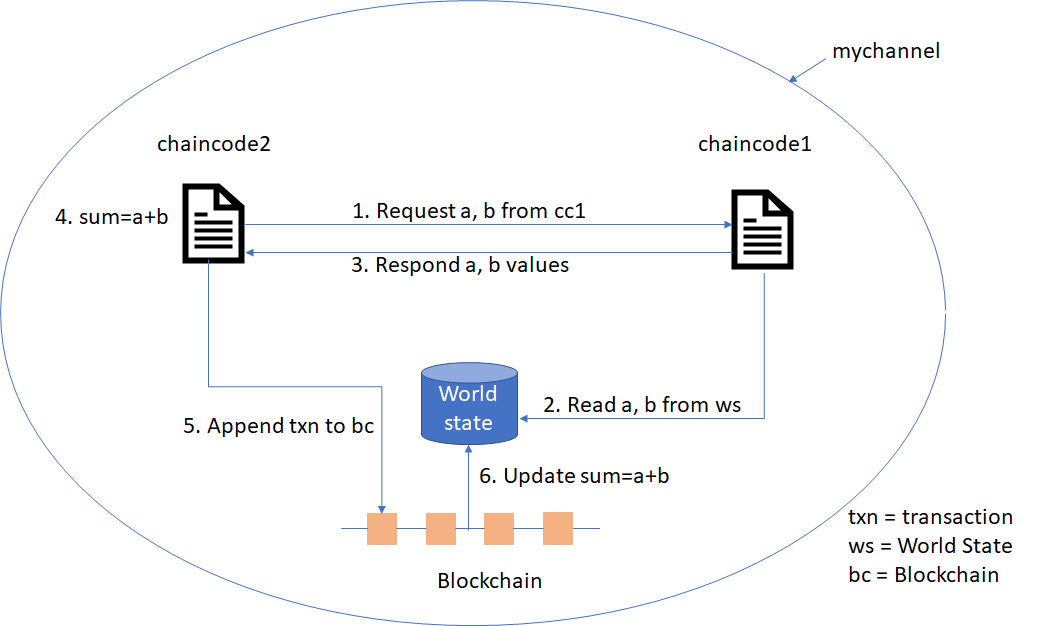
\includegraphics[width=\textwidth]{graphics/readsc.png}
\caption{The overall flow of read operation from a different chaincode}
\label{fig:readsc}
\end{center}
\end{figure}
The overall flow of the experiment can be seen in the Figure \ref{fig:readsc}. The figure shows the different operations that reads values from chaincode1 and returns those values to chaincode2 for further calculations.
\subsubsection{Results}
The above experiment to read the chaincode state from different chaincode can be summarized in the Table \ref{tab:result1}. The table shows the different values of the chaincode keys after different operations were performed. The key \textbf{sum} that belongs to \textbf{chaincode2} contains the sum of the values read for key \textbf{a} and the key \textbf{b} from \textbf{chaincode1}.
\begin{table}[h!]
\begin{center}
    \begin{tabular}{ |l|l|l|l|l|l|}
    \hline
    \multirow{2}{*}{\textbf{Keys}} & \multicolumn{5}{c|}{\textbf{Chaincode Operations}}\\ \cline{2-6}
    &\textbf{Install}& \textbf{Instantiate}& \textbf{Query}& \textbf{Invoke}& \textbf{Final Query} \\ \hline
    \textbf{a} & - & 100 & 100 & 90 & 90 \\ \hline
    \textbf{b} & - & 200 & 200 & 210 & 210 \\ \hline
    \textbf{sum} & - & 0 & 300 & 300 & 300 \\ \hline
    \end{tabular}
\end{center}
\caption{Different values for the keys during different chaincode operations.}
    \label{tab:result1}
\end{table}
\subsubsection{Conclusion of Results}
The experiment helps us to conclude that \begin{enumerate}
    \item A chaincode can read states of other chaincodes in the same channel with proper authorization.
    \item The caller chaincode, \textbf{chaincode2} interprets the object in the chaincode logic, and this object is not part of the MVCC for chaincode2 unless the caller chaincode writes it back to the ledger (using putState). 
    \item Any error in the called method of a different chaincode can be handled in the business logic of the caller chaincode that helps to create nested transactions characterized by read operations across different chaincodes that are both \textbf{atomic} and \textbf{consistent}.
\end{enumerate} 

\subsection{Write on same channel}
\label{ssec:wsc}
In the previous experiment, we have seen that chaincode can read state of another chaincode within the same channel. In this experiment, we will try to write to a chaincode state by executing a method of a different chaincode.

\subsubsection{Experimental setup}
For the experiment, we will use the same two chaincodes, \textbf{chaincode1} and \textbf{chaincode2} discussed in the previous subsection. However, we will create a new method in chaincode2 that writes a value to the keys belonging to chaincode1.

The method in chaincode2 will deduct value of key \textbf{a} by amount \textbf{x} and increase the value of key \textbf{b} by the same amount \textbf{x}. It is important to note that the operation will be called on \textbf{chaincode2} and the keys belong to \textbf{chaincode1}.
\begin{Listing}[h!]
\begin{lstlisting}
//write method for writing to chaincode1
func (t *SimpleChaincode) write(stub shim.ChaincodeStubInterface, args []string) pb.Response {
	var channelName string // channel Name
	var A, B string        // Entities
	var X int              // Transaction value
	var err1 error

	chaincodeName := args[0] // Expecting name of the chaincode you would like to call, this name would be given during chaincode install time
	A = args[1]
	B = args[2]
	X, err1 = strconv.Atoi(args[3])

	if len(args) > 2 {
		channelName = args[4]
	} else {
		channelName = ""
	}

	// invoke function of chaincode1 is called that puts A=A-X and B=B+X
	f := "invoke"
	queryArgs := toChaincodeArgs(f, A, B, strconv.Itoa(X))
	response := stub.InvokeChaincode(chaincodeName, queryArgs, channelName)
	if response.Status != shim.OK {
		errStr := fmt.Sprintf("Failed to query chaincode. Got error: %s", response.Payload)
		fmt.Printf(errStr)
		return shim.Error(errStr)
	}
	fmt.Printf("Query Response:%s\n", X)
	return shim.Success([]byte(strconv.Itoa(X)))
}
\end{lstlisting}
\caption{Code snippet for the \textit{write} method in the chaincode2}
\label{lst:cw}
\end{Listing}

In section \ref{sec:read}, we have already seen how the chaincodes are installed in listing \ref{lst:ci}, instantiated in listing \ref{lst:cin} and queried in listing \ref{lst:cq}. The new operation introduced in this section is invoking a method \textbf{write} that will write to chaincode1 state.

\subsubsection{Invoke chaincode}
\begin{Listing}[h!]
\begin{lstlisting}
peer chaincode invoke -o 127.0.0.1:7050 -C $CHANNEL_NAME -n chaincode1 -c '{"Args":["invoke","a","b","10"]}' //transfers 10 from a to b, a=90, b=210
peer chaincode invoke -o 127.0.0.1:7050 -C $CHANNEL_NAME -n chaincode2 -c '{"Args":["write","chaincode1","a","b","27","mychannel"]}' //calls the invoke method of chaincode1 that transfers 27 from a to b, a=63, b=237
\end{lstlisting}
\caption{cli command for chaincode \textit{invoke} with write operation}
\label{lst:winv}
\end{Listing}
\begin{figure}[h!]
\begin{center}
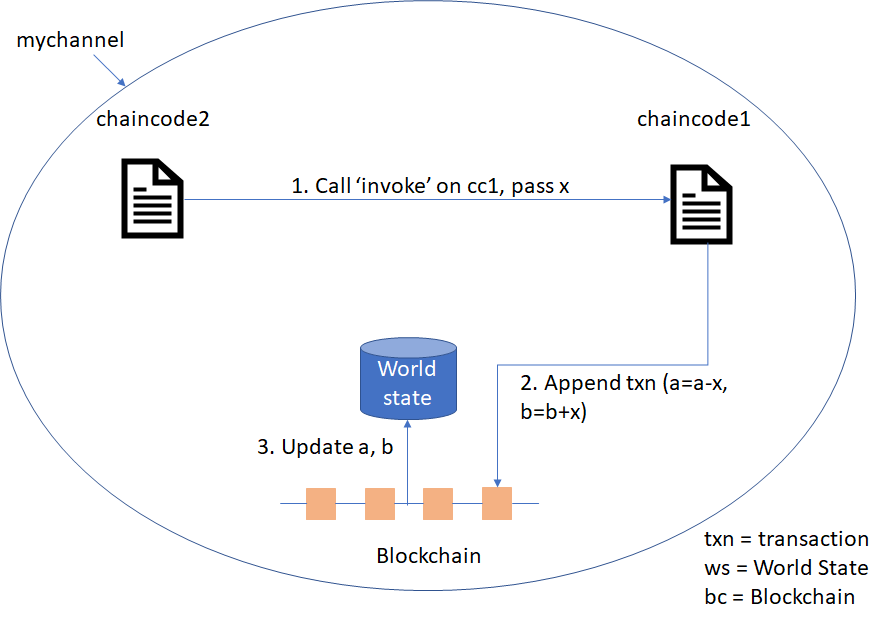
\includegraphics[width=\textwidth]{graphics/writesc.png}
\caption{The overall flow of write operation from a different chaincode}
\label{fig:writesc}
\end{center}
\end{figure}
The overall flow of the experiment can be seen in the Figure \ref{fig:writesc}. The figure shows the different operations that invokes method on chaincode1 which in turn writes the passed values from chaincode2 to the keys of chaincode1.

\subsubsection{Results}
The above experiment to write to the chaincode state from a  different chaincode can be summarized in the Table \ref{tab:result2}. The table shows the different values of the chaincode keys after different operations were performed. The keys \textbf{a} and \textbf{b} belong to \textbf{chaincode1} and their values are modified by calling a write operation from \textbf{chaincode2}.
\begin{table}[h!]
\begin{center}
    \begin{tabular}{ |l|l|l|l|l|l|}
    \hline
    \multirow{2}{*}{\textbf{Keys}} & \multicolumn{5}{c|}{\textbf{Chaincode Operations}}\\ \cline{2-6}
    &\textbf{Install}& \textbf{Instantiate}& \textbf{Query}& \textbf{Invoke\_cc1}& \textbf{Invoke\_cc2} \\ \hline
    \textbf{a} & - & 100 & 100 & 90 & 63 \\ \hline
    \textbf{b} & - & 200 & 200 & 210 & 237 \\ \hline
    \end{tabular}
\end{center}
\caption{Different values for the keys during different chaincode operations.}
\label{tab:result2}
\end{table}
\subsubsection{Conclusion of Results}
The experiment helps us to conclude that \begin{enumerate}
    \item A chaincode can write states to other chaincodes in the same channel with proper authorization.
    \item The key version check will take place for both the chaincodes in a single transaction context and if any check fails, the whole transaction will be termed as invalid. 
    \item Nested transactions spanning two different chaincodes can be considered as \textbf{atomic} and \textbf{consistent}.
\end{enumerate}

\section{Experiment 2: Chaincode to chaincode call on different channels}
In this section, we will perform the same experiment as in section \ref{sec:exp1} but the two chaincodes will be installed on different channels on a single peer.

\subsection{Read from different channels}
\label{subs:read2}
We will use the same two chaincodes,\textbf{chaincode1} and \textbf{chaincode2} discussed in the previous section. The goal will be to call a chaincode method to read its state that is present on a different channel but on the same peer.
\subsubsection{Experimental setup}
The steps are similar to what is described in section \ref{sec:read} with a major difference in the chaincode path. The \textbf{chaincode1} will be installed on \textbf{mychannel1} and \textbf{chaincode2} on \textbf{mychannel2} with the code in the two chaincodes remaining the same.

The \textbf{chaincode2} will invoke a method on \textbf{chaincode1} that queries and reads the states for keys, \textbf{a} and \textbf{b} belonging to chaincode1. These read values will be added and saved in the key \textbf{sum} belonging to chaincode2.

The different steps to perform the experiment can be highlighted as follows:
\subsubsection{Install chaincode}
\begin{Listing}[h!]
\begin{lstlisting}
//installs the chaincode1 with name as chaincode1 on channel mychannel1 and the chaincode file is located at the path specified by -p
peer chaincode install -n chaincode1 -C mychannel1 -v 1.0 -p github.com/chaincode/chaincode1/
//installs the chaincode2 with name as chaincode2 on channel mychannel2 and the chaincode file is located at the path specified by -p
peer chaincode install -n chaincode2 -v -C mychannel2 1.0 -p github.com/chaincode/chaincode2/
\end{lstlisting}
\caption{cli command for chaincode \textit{install}}
\label{lst:ci2}
\end{Listing}

\subsubsection{Instantiate chaincode}
\begin{Listing}[h!]
\begin{lstlisting}
//instantiates chaincode1 on channel mychannel1 with key a=100, b=200 and the endorsement policy is specified with -P, -o specifies the orderer endpoint
peer chaincode instantiate -o 127.0.0.1:7050 -C mychannel1 -n chaincode1 -v 1.0 -c '{"Args":["init","a", "100", "b","200"]}' -P "OR ('Org1MSP.member','Org2MSP.member')"

//instantiates chaincode2 on channel mychannel2 with key sum=0 and the endorsement policy is specified with -P, -o specifies the orderer endpoint
peer chaincode instantiate -o 127.0.0.1:7050 -C mychannel2 -n chaincode2 -v 1.0 -c '{"Args":["init","sum", "0"]}' -P "OR ('Org1MSP.member','Org2MSP.member')"
\end{lstlisting}
\caption{cli command for chaincode \textit{instantiate}}
\label{lst:cin2}
\end{Listing}
\subsubsection{Query chaincode}
\begin{Listing}[h!]
\begin{lstlisting}
peer chaincode query -C mychannel1 -n chaincode1 -c '{"Args":["query","a"]}' //response is a=100
peer chaincode query -C mychannel1 -n chaincode1 -c '{"Args":["query","b"]}' //response is b=200
//the args specifies in order the method in chaincode2 to call, the target callee chaincode name as chaincode1, the key in which value is stored and the channel name on which chaincode1 is installed which is mychannel1.
peer chaincode query -n chaincode2 -C mychannel2 -c '{"Args":["query","chaincode1","sum","mychannel1"]}' //response is sum=300
\end{lstlisting}
\caption{cli command for chaincode \textit{query}}
\label{lst:cq2}
\end{Listing}
\subsubsection{Invoke chaincode}
\begin{Listing}[h!]
\begin{lstlisting}
peer chaincode invoke -o 127.0.0.1:7050 -C mychannel1 -n chaincode1 -c '{"Args":["invoke","a","b","10"]}' //transfers 10 from a to b

peer chaincode invoke -o 127.0.0.1:7050 -C mychannel2 -n chaincode2 -c '{"Args":["invoke","chaincode1","sum","mychannel1"]}' //adds the value of a and b scoped to chaincode1 and saves sum=300 scoped to chaincode2
\end{lstlisting}
\caption{cli command for chaincode \textit{invoke}}
\label{lst:civ2}
\end{Listing}
\clearpage
\subsubsection{Final Query}
\begin{Listing}[h!]
\begin{lstlisting}
peer chaincode query -C mychannel1 -n chaincode1 -c '{"Args":["query","a"]}' //response is a=90
peer chaincode query -C mychannel1 -n chaincode1 -c '{"Args":["query","b"]}' //response is b=210
peer chaincode query -n chaincode2 -C mychannel2 -c '{"Args":["query","chaincode1","sum","mychannel1"]}' //response is sum=300
\end{lstlisting}
\caption{cli command for chaincode \textit{query}}
\label{lst:cf2}
\end{Listing}
\begin{figure}[h!]
\begin{center}
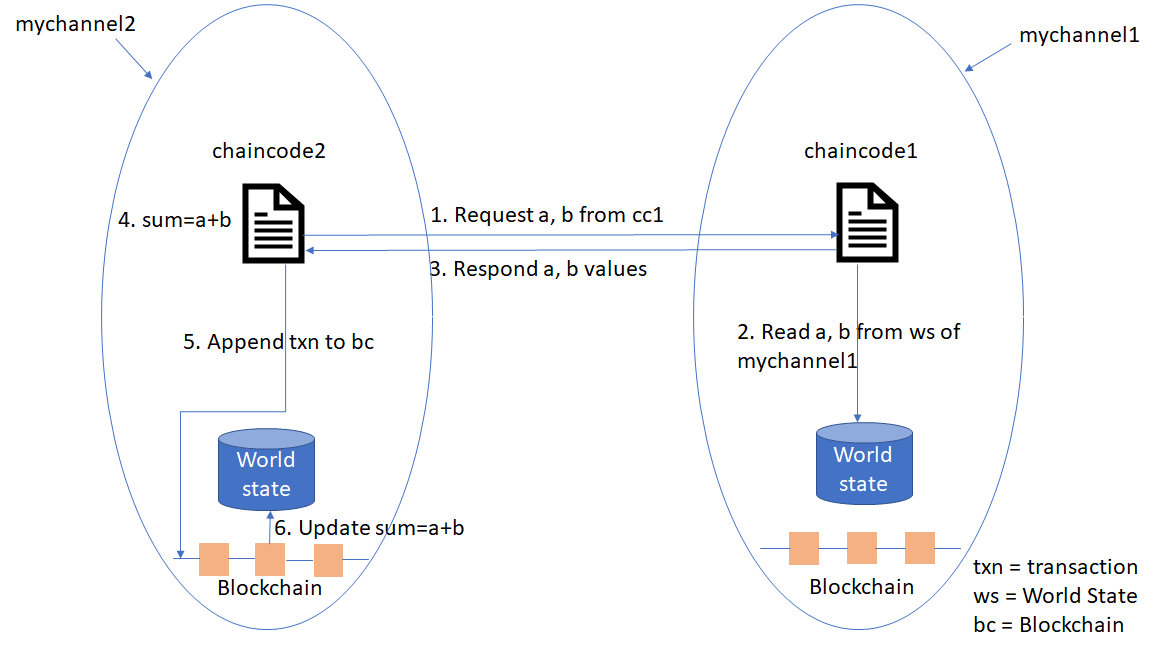
\includegraphics[width=\textwidth]{graphics/readsc2.png}
\caption{The overall flow of read operation from a different chaincode on different channels}
\label{fig:readsc2}
\end{center}
\end{figure}
The overall flow of the experiment can be seen in the Figure \ref{fig:readsc2}. The figure shows the different operations that reads values from chaincode1 and returns those values to chaincode2 for further calculations.
\subsubsection{Results}
\begin{table}[h!]
\begin{center}
    \begin{tabular}{ |l|l|l|l|l|l|}
    \hline
    \multirow{2}{*}{\textbf{Keys}} & \multicolumn{5}{c|}{\textbf{Chaincode Operations}}\\ \cline{2-6}
    &\textbf{Install}& \textbf{Instantiate}& \textbf{Query}& \textbf{Invoke}& \textbf{Final Query} \\ \hline
    \textbf{a} & - & 100 & 100 & 90 & 90 \\ \hline
    \textbf{b} & - & 200 & 200 & 210 & 210 \\ \hline
    \textbf{sum} & - & 0 & 300 & 300 & 300 \\ \hline
    \end{tabular}
\end{center}
\caption{Different values for the keys during different chaincode operations.}
    \label{tab:result12}
\end{table}
The above experiment to read the chaincode state from different chaincodes on different channels can be summarized in the Table \ref{tab:result12}. The table shows the different values of the chaincode keys after different operations were performed. The key \textbf{sum} that belongs to \textbf{chaincode2} on channel \textbf{mychannel2} contains the sum of the values read for key \textbf{a} and the key \textbf{b} from \textbf{chaincode1} that belongs on channel \textbf{mychannel1}. The experiment was also performed for different values of \textbf{a} and \textbf{b} and it concurred with the previous result.

\subsubsection{Conclusion of Results}
The experiment helps us to conclude that 
\begin{enumerate}
    \item A chaincode can read states of other chaincodes on different channels with proper authorization.
    \item The caller chaincode, \textbf{chaincode2} interprets the object in the chaincode logic, and this object is not part of the MVCC for chaincode2 unless the caller chaincode writes it back to the ledger (using putState). 
    \item Any error in the called method of a different chaincode can be handled in the business logic of the caller chaincode that can help to create nested transactions characterized by read operations across different chaincodes that are both \textbf{atomic} and \textbf{consistent}.
    \item The check will be based on read-write set of the callee chaincode, \textbf{chaincode1}, and hence, \textbf{chaincode2} should have read access for channel \textbf{mychannel1}.  
\end{enumerate} 

\subsection{Write on different channels}
In the previous experiment, we have seen that chaincode can read state of another chaincode present in a different channel. In this experiment, we will try to write to a chaincode state by executing a method of a different chaincode on a different channel.

\subsubsection{Experimental setup}
For the experiment, we will use the same two chaincodes, \textbf{chaincode1} and \textbf{chaincode2} discussed in the previous section and the method \textbf{write} discussed in listing \ref{lst:cw}.

We will call a method \textbf{write} defined in chaincode2 on channel \textbf{mychannel2}. The entire setup is similar to subsection \ref{ssec:wsc} with the only difference that chaincode1 will be on channel \textbf{mychannel1} and chaincode2 on \textbf{mychannel2}. 

The steps include Install, Instantiate, Query, Invoke and Final Query as outlined in previous subsection. Lets see the Invoke and Query results.
\clearpage
\subsubsection{Invoke chaincode}
\begin{Listing}[h!]
\begin{lstlisting}
peer chaincode invoke -o 127.0.0.1:7050 -C mychannel1 -n chaincode1 -c '{"Args":["invoke","a","b","10"]}' //transfers 10 from a to b, a=90, b=210
peer chaincode invoke -o 127.0.0.1:7050 -C mychannel2 -n chaincode2 -c '{"Args":["write","chaincode1","a","b","27","mychannel1"]}' //the write results in no change to values of a and b, a=90 and b=210
\end{lstlisting}
\caption{cli command for chaincode \textit{invoke} with write operation on different channels}
\label{lst:winv2}
\end{Listing}
\begin{figure}[h!]
\begin{center}
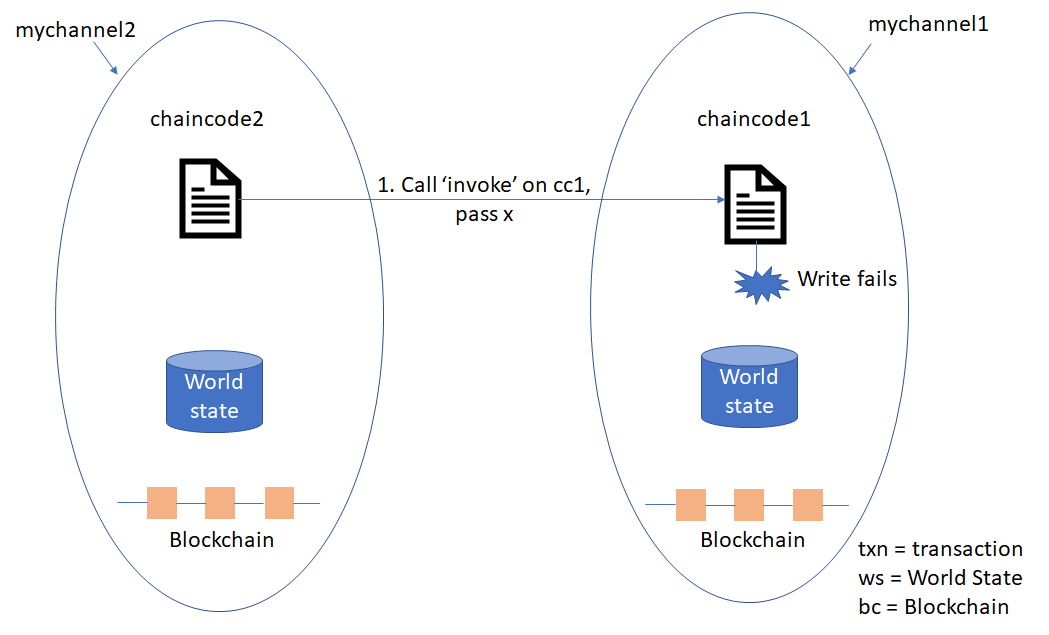
\includegraphics[width=\textwidth]{graphics/writesc2.png}
\caption{The overall flow of write operation from a different chaincode on a different channel}
\label{fig:writesc2}
\end{center}
\end{figure}
The overall flow of the experiment can be seen in the Figure \ref{fig:writesc2}. The figure shows the different operations that invokes method on chaincode1 which in turn tries to update the state of chaincode1 on channel \textbf{mychannel1}.

\subsubsection{Results}
The above experiment to write to the chaincode state from a  different chaincode on a different channel can be summarized in the Table \ref{tab:result22}. The table shows the different values of the chaincode keys after different operations were performed. The keys \textbf{a} and \textbf{b} belong to \textbf{chaincode1} on channel \textbf{mychannel1}.
\begin{table}[h!]
\begin{center}
    \begin{tabular}{ |l|l|l|l|l|l|}
    \hline
    \multirow{2}{*}{\textbf{Keys}} & \multicolumn{5}{c|}{\textbf{Chaincode Operations}}\\ \cline{2-6}
    &\textbf{Install}& \textbf{Instantiate}& \textbf{Query}& \textbf{Invoke\_cc1}& \textbf{Invoke\_cc2} \\ \hline
    \textbf{a} & - & 100 & 100 & 90 & 90 \\ \hline
    \textbf{b} & - & 200 & 200 & 210 & 210 \\ \hline
    \end{tabular}
\end{center}
\caption{Different values for the keys during different chaincode operations.}
\label{tab:result22}
\end{table}
\subsubsection{Conclusion of Results}
The experiment helps us to conclude that 
\begin{enumerate}
\item A chaincode on one channel cannot write to a chaincode state on a different channel.
\item Since every channel maintains its own ledger, it is not possible to update the state in a different channel.
\item In case a transaction consists of multiple sub-transactions, a 2-PC transaction monitor will be required that will manage the atomic commits and keep the blockchain and world state consistent.
\end{enumerate}

\section{Experiment 3: Implementation of an intermediate layer for transaction management}
In the previous sections, we were able to conclude that chaincode to chaincode write is not possible if the two chaincodes are on separate channels. Channels in Hyperledger Fabric are created to provide data privacy to the member of that channel and hence, an external write request fails \cite{Channels}. But a business transaction may include scenarios that require write on different channels and within the same transaction context. In short, a large business transaction may consist of smaller transactions that have write operations on different channels.

There are different alternatives with the use of channels as discussed down below:
\begin{enumerate}
    \item Use of a single channel and private data collection to provide privacy for only the data that is sensitive and cannot be shared with other peers on the channel. It will serve the purpose of multiple channels for data confidentiality.
    \item Use of single channel with data encryption.
    \item Use of multiple channels with an intermediate implementation of a software layer like a 2-PC transaction monitor on the application side that has access to all the channel's data and manages the dependent transactions. This layer has to take care of \textbf{rollback}, \textbf{compensation action} and \textbf{commit} for all the transactions. However, this type of implementation will make the network slow.
\end{enumerate}

We will focus on the third approach above and create a software implementation on the client application that handles multiple transactions within a single transaction context.

\subsection{Use case scenario}
Consider a scenario involving a large business transaction spanning 2 channels, \textbf{mychannel2} and \textbf{mychannel3}. Consider there is a \textbf{supplier1} and \textbf{company1} on \textbf{mychannel2} and \textbf{supplier2} and \textbf{company1} on \textbf{mychannel3}. Now consider a large business transaction such that the price on \textbf{mychannel2} for a product will be reduced if and only if the price of the product can be increased on \textbf{mychannel3}. These are 2 sub-transactions part of a large single business transaction. Since, we cannot write to a different channel, a software implementation that manages the transaction is developed. The developed software implementation is an extension of the application developed in chapter \ref{chap:cs}.
\begin{figure}[h!]
\begin{center}
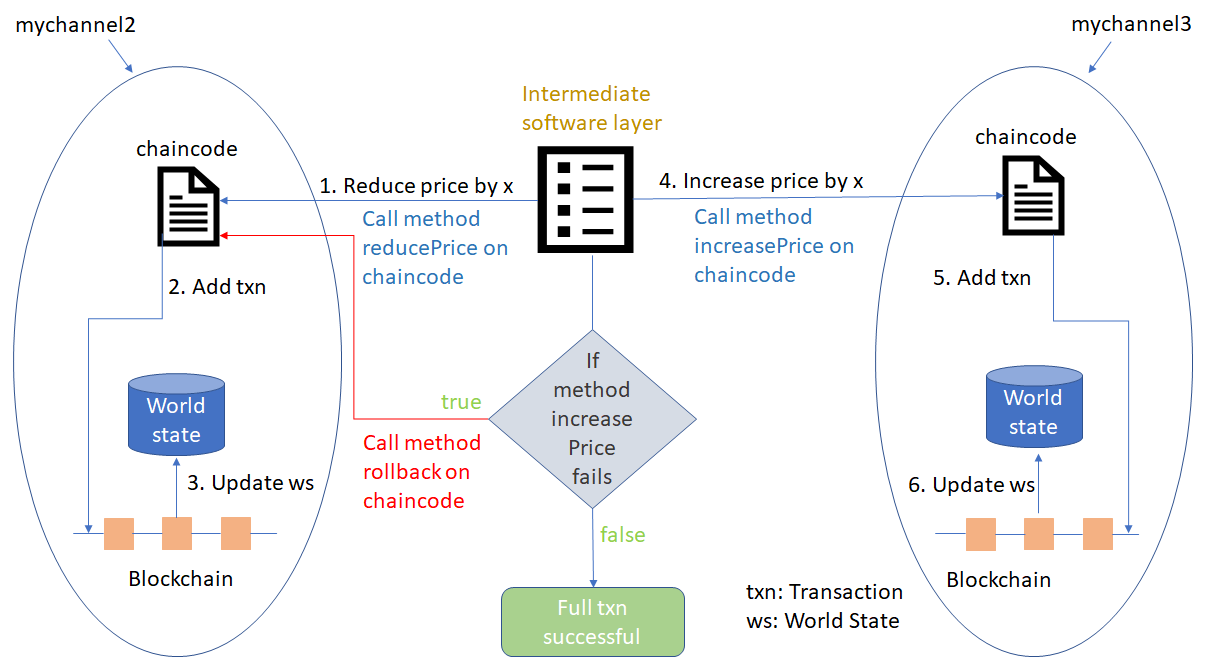
\includegraphics[width=\textwidth]{graphics/2pcDiagram.png}
\caption{The overall flow of two separate transactions managed within a single transaction context. }
\label{fig:2pcDiagram}
\end{center}
\end{figure}

Figure \ref{fig:2pcDiagram} shows the system with two different channels. Let us discuss the design of the software layer.
\begin{enumerate}
    \item The entire transaction to reduce price on \textbf{mychannel2} and increase price on \textbf{mychannel3} is a single transaction that has to be managed as two sub-transactions by the intermediate software layer.
    \item The transaction starts by reducing price on channel \textbf{mychannel2}. This is achieved by calling the chaincode method \textbf{reducePrice}. At the same time, the last value for price before reducing it on \textbf{mychannel2} is saved in a \textbf{localStorage} string variable and a boolean variable that stores if \textbf{increasePrice} was successful or not.
    \item When the \textbf{increasePrice} method is called, the boolean variable \textbf{isPriceIncreased} is set to true. This marks the completion of entire transaction.
    \item However, there are cases when the transaction for increasing price fails. In that scenario, the boolean variable \textbf{isPriceIncreased} is set to false. The software layer checks regularly if the \textbf{increasePrice} method was successfully executed. If its not successfully executed, a new transaction on \textbf{mychannel2} is submitted that puts the old price in the world state of \textbf{mychannel2}. This is mimicking the \textbf{rollback} transaction but with a \textbf{compensation action} as a blockchain is an append-only ledger.
    \item Similar check can be carried out for \textbf{reducePrice} as the order of transaction does not matter and in order that the entire transaction is successful, both the transactions should successfully be committed to their respective ledgers.
    \item Thus the software layer works like a 2-PC transaction monitor for transaction management of multiple sub-transactions spanning different channels.
\end{enumerate}
\begin{figure}[h!]
\begin{center}
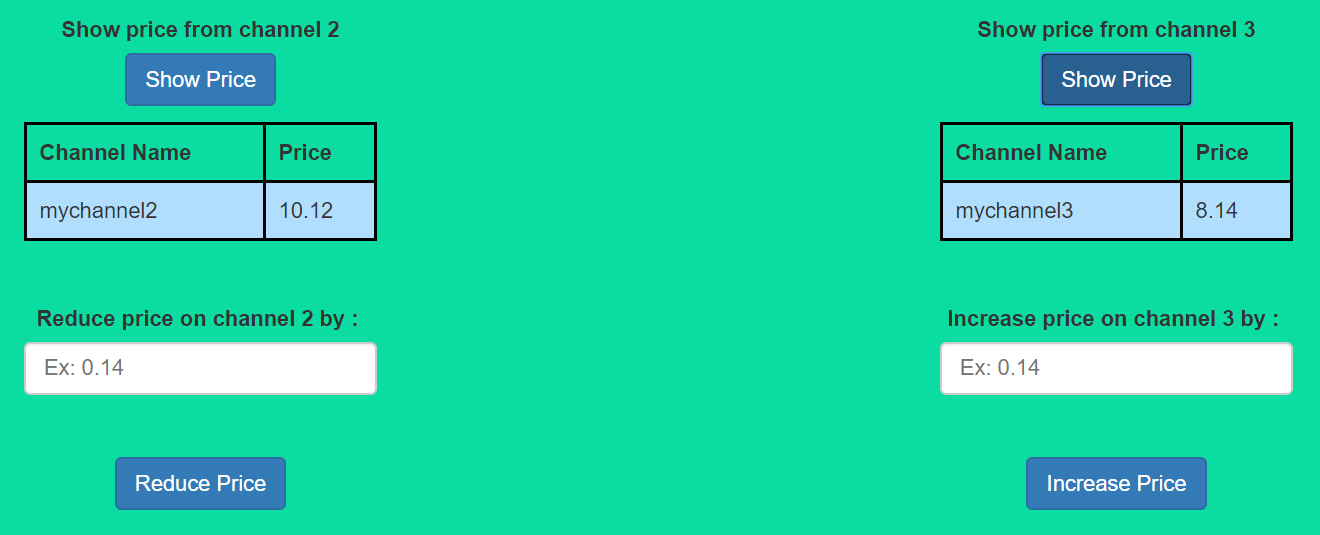
\includegraphics[width=\textwidth]{graphics/2pc.png}
\caption{The view of the software layer that handles transaction on multiple channels. }
\label{fig:2pc}
\end{center}
\end{figure}
Figure \ref{fig:2pc} shows the view that helped to conduct the experiment. The two actions, to reduce price and increase price, are put on respective button clicks as shown in the figure for experimentation. However, in real scenarios this will be a single event and can be managed by execution of one method after another with \textbf{callback}.

\subsection{Results}
With the help of this experiment, the price on both the channels was changed and this was part of a single transaction context. Write on a different channel is not allowed, but with an intermediate software layer we were able to manage transactions spanning multiple channels. It is also possible to rollback the transaction effects on the world state with proper implementation. However, a rollback transaction on the blockchain involves submitting a new transaction that is also recorded on the blockchain as it is an append-only ledger. 

\subsection{Conclusion of Results}
It is possible to manage transactions spanning different channels. However, this makes the system slow due to an intermediate layer and should be implemented only when it is absolutely essential. It is possible to rollback the transaction effect by submitting a new transaction. In short, the rollback works on the world state and not on the blockchain.

\section{Experiment 4: Test for immutability of ledger}
The experiments that were performed till now were related to channels and chaincodes. In this experiment, we will focus on the immutability of blockchain component of ledger and also try to change the world state without invoking any chaincode transactions. This experiment will help us to understand how strong is the immutability property of blockchains compared to durability in ACID transactions.

\subsection{Modifying the world state}
In this experiment we will create a blockchain network with two peers, \textbf{PEER0} belonging to \textbf{Organization1} and \textbf{PEER2} belonging to \textbf{Organization2}. Both the peers will be part of a single channel \textbf{mychannel} and endorsement policy will be set to \textit{OR ('Org1MSP.member','Org2MSP.member')}.

This experiment is based on the \textbf{marbles} example designed by the Hyperledger Fabric community \cite{marbles}. We will use the same setting to test the world state with couchDB container.

Steps to perform the experiment and the corresponding outcome for each step can be outlined as follows:
\begin{enumerate}
    \item Joined both the peers, \textbf{PEER0} and \textbf{PEER1} to the channel \textbf{mychannel}.
    
    \textbf{Outcome}: The world state is populated in a separate container and can be accessed in the browser through the port specified in the docker-compose file. However, it is important to note that world state is only visible when the peers join the channel.
    \item An invoke transaction is submitted from \textbf{PEER0} that creates a marble, \textbf{marble1} {\ttfamily\bfseries\slshape \{name:"marble1", size:"20", color:"blue", owner:"vikas"\}}
    
    \textbf{Outcome}: The created marble can be seen for each of the peers in their respective containers. At this stage, all the peers have consistent copy of data.
    \item The value for \textbf{color} field of \textbf{marble1} is changed to \textbf{green} by manually modifying the object in the couchDB host for \textbf{PEER0}.
    
    \textbf{Outcome}: A query for \textbf{marble1} on \textbf{PEER0} gave the manually modified value with \textbf{color} as \textbf{green} while a query on \textbf{PEER2} gave the value for \textbf{color} as \textbf{blue} that is the correct one. This shows that the peers are in inconsistent state.
    \item There is a function in the \textbf{marbles} chaincode called as \textbf{transferMarblesBasedOnColor} that checks the color of the marble and changes its owner. Called this method from \textbf{PEER0} to change the owner to "Ghareeb" for marbles of color \textbf{green} (this is the modified color value on PEER0, and PEER2 holds the right value for color as blue). 
    
    \textb{Outcome}: There is no change in owner on any of the peers even when the \textb{PEER0} had manually modified color value as \textb{green}.
    \item Called the same function \textbf{transferMarblesBasedOnColor} on \textbf{PEER0} but now the color value was \textb{blue} (that is the right one) and new owner as "Ghareeb".
    
    \textb{Outcome}: Though the \textb{owner} was changed to "Ghareeb", the \textb{color} field also got modified to \textb{green} (this is wrong value) on both the peers. The data was consistent on both the peers but the color field was incorrect. So instead of {\ttfamily\bfseries\slshape \{name:"marble1", size:"20", color:"blue", owner:"Ghareeb"\}}, it showed {\ttfamily\bfseries\slshape \{name:"marble1", size:"20", color:"green", owner:"Ghareeb"\}}
\end{enumerate}

\subsubsection{Conclusion of Results}
\begin{enumerate}
    \item The above experiment showed that a peer's world state can be accessed and modified leading inconsistent state on that peer. Authentication for the couchDB container should be provided so that unauthorized changes in world state can be avoided. This can be achieved by creating username and password for the admin account.
    \item It was seen that the malicious peers data can affect the data of all the peers in the blockchain and lead to an \textb{inconsistent} state. The solution for this would be to use a stronger endorsement policy requiring endorsements from multiple peers of all the organizations. Care should be taken to install chaincode on all the endorsing peers (endorsement is generate by executing a transaction and transactions can only be executed by the chaincode).
\end{enumerate}

\subsection{Modifying the peer blockchain}
In this experiment, we will try to modify the blockchain file present on the peer and see its effect on query and invoke transactions. The blockchain on a peer container is located at \textb{var/hyperledger/production/ledgersData/chains/chains/mychannel}. Here mychannel is the name of the channel. We will modify the blockchain file for a peer and see its effect.

The same example of \textb{marbles} \cite{marbles} can be used as discussed above. The steps for the experiment can be outlined as follows:
\begin{enumerate}
    \item Joined \textb{PEER0} to the channel, \textbf{mychannel} and created a marble object \textbf{marble1} with fields as {\ttfamily\bfseries\slshape \{name:"marble1", size:"20", color:"blue", owner:"vikas"\}}
    
    \textb{Outcome}: The \textbf{marble1} object was created and after querying fetched the right results. There is a method called \textbf{getHistoryForMarble} that queries the blockchain for the transaction ids related to the marble name. This method also returned the right transaction id.
    \item The blockchain file on \textbf{PEER0} was located at {\ttfamily\bfseries\slshape var/hyperledger/production/ledgersData/} and was copied on the desktop to view its content. Then a new transaction was submitted for \textbf{marble2} on the same peer with fields as {\ttfamily\bfseries\slshape \{name:"marble2", size:"70", color:"red", owner:"ghareeb"\}}.
    
    \textbf{Outcome}: The data was consistent and both the marbles object were visible in the couchDB container and the query also fetched right results.
    \item Then copied the blockchain file with the new transaction for \textbf{marble2} on the desktop. Compared the contents of the two blockfiles. Removed the recently added block from new file that had the transaction for \textbf{marble2} and saved this file in the \textbf{PEER0} container. Queried the world state for the \textbf{marble2} and the blockchain with the method \textbf{getHistoryForMarble} for \textbf{marble2}.
    
    \textbf{Outcome}: It was found that a query on world state fetched the right result for \textbf{marble2}. However, \textbf{getHistoryForMarble} that queries the blockchain for \textb{marble2} history gave an endorsement failure error. This demonstrates that the blockchain on \textbf{PEER0} has been tampered with.
    \item Joined a new peer, \textbf{PEER2} to the channel and executed the method \textbf{getHistoryForMarble}. 
    
    \textbf{Outcome}: The query executed without errors and contained the transaction history for \textbf{marble1} and \textbf{marble2} executed separately. This indicates that when a new peer joins the channel, its blockchain is created and synced through the blocks in the \textbf{orderer} node. 
    
\end{enumerate}
\subsubsection{Conclusion of Results}
\begin{enumerate}
    \item Modifying the blockchain on a peer can be detected and the malicious peer can be removed from the network.
    \item The queries on keys are executed only on the world state and hence, it is decoupled from the blockchain for queries. Even if the blockchain has been tampered, the world state still contains the right values.
    \item A new joining peer will never get the tampered blocks and will always contain consistent data.
\end{enumerate}

\subsection{Modifying the peer and orderer blockchain and then joining a new peer}
In this subsection, we will modify the blockchain for two peers, \textb{PEER0} and \textbf{PEER2} on the channel, then we will modify the orderer blockchain and then join two new peers, \textbf{PEER1} belonging to \textbf{Org1} and \textbf{PEER3} belonging to \textbf{Org2}. The same example of \textbf{marbles} as in the previous subsections will be used \cite{marbles}. 
\begin{Listing}[h!]
\begin{lstlisting}
    marble1 {name:"marble1", color: "blue", owner: "vikas", size:"70"}
    marble2 {name:"marble2", color: "green", owner: "ghareeb", size:"70"}
    marble3 {name:"marble3", color: "red", owner: "jason", size:"70"}
    marble4 {name:"marble4", color: "blue", owner: "bhuppi", size:"70"}
    marble5 {name:"marble5", color: "blue", owner: "romeet", size:"70"}
\end{lstlisting}
\caption{The different objects created in the experiment}
\label{lst:obj}
\end{Listing}

Listing \ref{lst:obj} shows the different objects that will be created in separate transactions in the network. In the remaining part, we will refer to the objects with their \textbf{name} fields. In total five invoke transactions will be executed on the network at different times after modifying the blockchain file.

The different steps in the experiment and their corresponding analysis can be highlighted as below:

\begin{enumerate}
    \item Joined \textbf{PEER0} and \textbf{PEER2} to the channel \textbf{mychannel}. Submitted three transactions for \textbf{marble1}, \textbf{marble2} and \textbf{marble3} respectively.
    
    \textbf{Outcome}: The three transactions were visible on both the peers and query on the blockchain and world state yielded correct results.
    \item Removed the block that contained the transaction for \textbf{marble3} from the blockchain file of \textbf{PEER0}. The blockchain file is located at {\ttfamily\bfseries\slshape var/hyperledger/production/ledgersData/..}.
    
    \textbf{Outcome}: Execution of method \textbf{getHistoryForMarble} on \textbf{PEER0} for \textbf{marble1} and \textbf{marble2} yielded correct results. However, execution of this method for \textbf{marble3} yielded endorsement failure error. Verified it again by running the method for all the three marbles on \textbf{PEER2} which yielded right results. Thus, the \textbf{PEER0} blockchain file has been tampered can be identified.
    \item Created another transaction for a new marble, \textbf{marble4}.
    
    \textbf{Outcome}: The world state for the four marbles showed correct data in the couchDB container for both the peers. However, the \textbf{getHistoryForMarble} method on \textbf{PEER0} for \textbf{marble4} gave the endorsement failure error.
    \item Removed the block for the transaction containing \textbf{marble4} from \textbf{PEER2}.
    
    \textbf{Outcome}:The same behaviour of endorsement failure was observed here on \textbf{PEER2} after the execution of the method \textbf{getHistoryForMarble}.
    \item Submitted another transaction that created a new marble, \textbf{marble5} on the network.
    
    \textbf{Outcome}: The transactions was successful an the couchDB container for both the peers showed five different marble objects.
    \item Removed the block containing the transaction for \textbf{marble5} from the orderer blockchain file. The orderer blockchain file is present at {\ttfamily\bfseries\slshape var/hyperledger/production/orderer/..}. Joined peer \textbf{PEER1} to the channel.
    
    \textbf{Outcome} Initially when the peer \textbf{PEER1} joined the channel, it contained only three marble objects, \textbf{marble1}, \textbf{marble2} and \textbf{marble3}. However, the blockchain got synced after a considerable amount of time and showed all the five marble objects. Execution of the method \textbf{getHistoryForMarble} for all the five marbles yielded the right results.
    \item Joined peer \textbf{PEER3} to the channel.
    
    \textbf{Outcome}: Initially it showed only four marble objects, \textbf{marble1}, \textbf{marble2}, \textbf{marble3} and \textbf{marble4} but eventually synced to all the five objects. Execution of the method \textbf{getHistoryForMarble} for all the five marbles yielded the right results.
\end{enumerate}
\subsubsection{Conclusion of Results}
\begin{enumerate}
    \item It can be seen that initially the newly joining peers were not consistent, but eventually they synced their blockchain files and contained the right blocks even after the orderer and the peer blockchain files were modified.
    \item This leads us to believe that any tampering with the blockchain files can be easily caught by the system and the system tries to reach a consistent state eventually.
    \item The ledger can, thus, be considered as tamper-resistant.
    \item The experiment can be further extended to test for immutability by adopting different approaches.
\end{enumerate}
\chapter{Conclusion}
In this chapter we will finally conclude the entire thesis. In the first part we will discuss the summary of the tasks done and the second part will focus on the future work that can be done to further study the blockchain networks.
\label{chap:cf}

\section*{Summary}
The aim of this thesis was to study the transaction characteristics of permissioned blockchain network. For the purpose of the study, we used Hyperledger Fabric that contains a highly modular architectural pattern. We have seen the various components like \textit{chaincodes}, \textit{channels}, \textit{endorsement policies}, and the \textit{consensus protocols} in a permissioned blockchain network. The transactional properties are affected by these components and hence, importance was given to create strong modular components. 

The first part of the thesis mainly focused on the research aspects related to consensus algorithms, comparing the transactional properties of permissioned blockchain networks with that of the permissionless networks and also to ACID transactions. The later part was mainly focused on how a permissioned blockchain works with all the components and the experiments that helped us to understand certain important transactional aspects. 

It can be concluded that a blockchain system has an tamper-proof ledger and any modifications in the blockchain does not affect newly added peers. However, a modification to the world state and without a strong endorsement policy can lead to unwanted data being committed to the blockchain and the world state. Also writes on different channels can be achieved in business transactions by implementing an intermediate software layer that mimics a 2-PC transaction monitor where a large transaction consisting of multiple sub-transactions is made \textbf{atomic}. 

\section*{Future Work}
A blockchain network can have multiple organizations adopting different blockchain frameworks and hence, it becomes necessary to adopt a dynamic solution for blockchain networks. Further study can be done to understand the interaction of different blockchain networks like Ethereum and Hyperledger Fabric that can make the blockchain environment more interesting. Work can be done to study the transactional properties of business transactions in mixed blockchain environment.

Also the immutability of the blockchain can be made more stronger by implementing compulsory strong endorsement policies and not leaving it to the disposal of the developer. A huge problem of networks like Hyperledger Fabric is the certificate authority which is currently a single node (therefore representing a single point of failure on the network) and this can be researched further.
%\blinddocument

\printbibliography

\appendix
%% !TeX root = main-english.tex
% !TeX spellcheck = en-US
% !TeX encoding = utf8
% -*- coding:utf-8 mod:LaTeX -*-

%This smart spell only works if no changes have been made to the chapter 
%using the options proposed in preambel/chapterheads.tex.
\setchapterpreamble[u]{%
  \dictum[Albert Einstein]{We cannot solve our problems with the same level of thinking that created them}
}
\chapter{LaTeX Hints}
\label{chap:latexhints}

One sentence per line.
This rule is important for the usage of version control systems.
A new line is generated with a blank line.
As you would do in Word:
New paragraphs are generated by pressing enter.
In LaTeX, this does not lead to a new paragraph as LaTeX joins subsequent lines.
In case you want a new paragraph, just press enter twice (!).
This leads to an empty line.
In word, there is the functionality to press shift and enter.
This leads to a hard line break.
The text starts at the beginning of a new line.
In LaTeX, you can do that by using two backslashes (\textbackslash\textbackslash).
This is rarely used.

Please do \textit{not} use two backslahes for new paragraphs.
For instance, this sentence belongs to the same paragraph, whereas the last one started a new one.
A long motivation for that is provided at \url{http://loopspace.mathforge.org/HowDidIDoThat/TeX/VCS/#section.3}.

\section{File Encoding and Support of Umlauts}
\label{sec:firstsectioninlatexhints}
The template offers foll UTF-8 support.
All recent editors should not have issues with that.

\section{Citations}


References are set by means of \texttt{\textbackslash cite[key]}.

\begin{filecontents*}{\democodefile}
Example: \cite{WSPA} or by author input: \citet{WSPA}.
\end{filecontents*}
\PrintDemo{style=parallel}

The following sentence demonstrates
\begin{inparaenum}[1.]
  \item the capitalization of author names at the beginning of the sentence,
  \item the correct citation using author names and the reference,
  \item that the author names are a hyperlink to the bibliography and that
  \item the bibliography contains the name prefix \qq{van der} of \qq{Wil M.\,P.\ van der Aalst}.
\end{inparaenum}

\begin{filecontents*}{\democodefile}
\Citet{RVvdA2016} present a study on the effectiveness of workflow management systems.
\end{filecontents*}
\PrintDemo{style=parallel}

The following sentence demonstrates that you can overwrite the text part of the generated label using \texttt{label} in a bibliopgrahie"=entry, but the year and the uniqueness is still generated by biber.

\begin{filecontents*}{\democodefile}
The workflow engine Apache ODE \cite{ApacheODE} executes \BPEL processes reliably.
\end{filecontents*}
\PrintDemo{style=parallel}

\begin{filecontents*}{\democodefile}
Words are best enclosed using \texttt{\textbackslash qq\{..\}}, then the correct quotes are used.
\end{filecontents*}
\PrintDemo{style=parallel}

When creating the Bibtex file it is recommended to make sure that the DOI is listed.

\section{Formulas and Equations}
\label{sec:mf}

\begin{filecontents*}{\democodefile}
Equations $f(x)=x$ inside the text can be provided.
\end{filecontents*}
\PrintDemo{style=parallel}

A list with all available mathematical symbols is provided at \url{http://texdoc.net/pkg/symbols-a4}.

\begin{filecontents*}{\democodefile}
As example the set of natural numbers is given by $\mathbb{N}$.
\end{filecontents*}
\PrintDemo{style=parallel}

For the documentation of editing mathematical formulas read the package documentation of \texttt{amsmath}\footnote{\url{http://texdoc.net/pkg/amsmath}}.

Equation~\ref{eq:test} is numbered and can be referenced in the text:
\begin{filecontents*}{\democodefile}
\begin{align}
  \label{eq:test}
  x = y
\end{align}
\end{filecontents*}
\PrintDemo{style=parallel}

Following equation is not numbered because of using \texttt{\textbackslash align*} as environment.
\begin{filecontents*}{\democodefile}
\begin{align*}
  x = y
\end{align*}
\end{filecontents*}
\PrintDemo{style=parallel}

The template offers \verb+\abs+ to enable the bars scaling well at the absolute value:

\begin{filecontents*}{\democodefile}
$\abs{X}$.
\end{filecontents*}
\PrintDemo{style=parallel}

More details about mathematical environments provides the documentation available at \url{http://www.ctan.org/tex-archive/help/Catalogue/entries/voss-mathmode.html}.


%%%%%%%%%%%%%%%%%%%%%%%%%%%%%%%%%%%%%%%%%%%%%%%%%%%%%%%%%%%%%%%%%%%%%%%%%%%%%%
\section{Sourcecode}
%%%%%%%%%%%%%%%%%%%%%%%%%%%%%%%%%%%%%%%%%%%%%%%%%%%%%%%%%%%%%%%%%%%%%%%%%%%%%%
\Cref{lst:ListingANDlstlisting} shows how to emmbed source code.
With \texttt{\textbackslash lstinputlisting} the source code can be loaded directly from files.

%Listing-Umgebung wurde durch \newfloat{Listing} definiert
\begin{Listing}
  \begin{lstlisting}
<listing name="second sample">
  <content>not interesting</content>
</listing>
\end{lstlisting}
  \caption{The code is separated by two horizontal lines in the listings environment.}
  \label{lst:ListingANDlstlisting}
\end{Listing}

\begin{filecontents*}{\democodefile}
Source code is also available in the text \lstinline|<listing />|.
\end{filecontents*}
\PrintDemo{style=parallel}


%%%%%%%%%%%%%%%%%%%%%%%%%%%%%%%%%%%%%%%%%%%%%%%%%%%%%%%%%%%%%%%%%%%%%%%%%%%%%%
\section{Pseudocode}
%%%%%%%%%%%%%%%%%%%%%%%%%%%%%%%%%%%%%%%%%%%%%%%%%%%%%%%%%%%%%%%%%%%%%%%%%%%%%%
\Cref{alg:sample} shows a sample algorithm.
\begin{Algorithmus} %Use the environment only if you want to place the algorithm similar to graphics from TeX
  \caption{Sample algorithm}
  \label{alg:sample}
  \begin{algorithmic}
\Procedure{Sample}{$a$,$v_e$}
\State $\mathsf{parentHandled} \gets (a = \mathsf{process}) \lor \mathsf{visited}(a'), (a',c,a) \in \mathsf{HR}$
\State \Comment $(a',c'a) \in \mathsf{HR}$ denotes that $a'$ is the parent of $a$
\If{$\mathsf{parentHandled}\,\land(\mathcal{L}_\mathit{in}(a)=\emptyset\,\lor\,\forall l \in \mathcal{L}_\mathit{in}(a): \mathsf{visited}(l))$}
\State $\mathsf{visited}(a) \gets \text{true}$
\State $\mathsf{writes}_\circ(a,v_e) \gets
\begin{cases}
\mathsf{joinLinks}(a,v_e) & \abs{\mathcal{L}_\mathit{in}(a)} > 0\\
\mathsf{writes}_\circ(p,v_e)
& \exists p: (p,c,a) \in \mathsf{HR}\\
(\emptyset, \emptyset, \emptyset, false) & \text{otherwise}
\end{cases}
$
\If{$a\in\mathcal{A}_\mathit{basic}$}
  \State \Call{HandleBasicActivity}{$a$,$v_e$}
\ElsIf{$a\in\mathcal{A}_\mathit{flow}$}
  \State \Call{HandleFlow}{$a$,$v_e$}
\ElsIf{$a = \mathsf{process}$} \Comment Directly handle the contained activity
  \State \Call{HandleActivity}{$a'$,$v_e$}, $(a,\bot,a') \in \mathsf{HR}$
  \State $\mathsf{writes}_\bullet(a) \gets \mathsf{writes}_\bullet(a')$
\EndIf
\ForAll{$l \in \mathcal{L}_\mathit{out}(a)$}
  \State \Call{HandleLink}{$l$,$v_e$}
\EndFor
\EndIf
\EndProcedure
  \end{algorithmic}
\end{Algorithmus}

\clearpage
And if you want to write an algorithm that goes over several pages, you can only do this with the following \textbf{dirty} hack:

{
\begin{minipage}{\textwidth}
  \hrule height .8pt width\textwidth
  \vskip.3em%\vskip\abovecaptionskip\relax
  \stepcounter{Algorithmus}
  \addcontentsline{alg}{Algorithmus}{\protect\numberline{\theAlgorithmus}{\ignorespaces Description \relax}}
  \noindent\textbf{Algorithmus \theAlgorithmus} Description
  %\stepcounter{algorithm}
  %\addcontentsline{alg}{Algorithmus}{\thealgorithm{}\hskip0em Description}
  %\textbf{Algorithmus \thealgorithm} Description
  \vskip.3em%\vskip\belowcaptionskip\relax
  \hrule height .5pt width\textwidth
\end{minipage}
%without the following line, the text is nerer at the rule
\vskip-.3em
%
code goes here\\
test2\\
%
\vskip-.7em
\hrule height .5pt width\textwidth
}


%%%%%%%%%%%%%%%%%%%%%%%%%%%%%%%%%%%%%%%%%%%%%%%%%%%%%%%%%%%%%%%%%%%%%%%%%%%%%%
\section{Figures}
%%%%%%%%%%%%%%%%%%%%%%%%%%%%%%%%%%%%%%%%%%%%%%%%%%%%%%%%%%%%%%%%%%%%%%%%%%%%%%
The \cref{fig:chor1} and \ref{fig:chor2} are important to understand this document.
In the appendix \vref{fig:AnhangsChor} shows again the complete choreography.

%The parameters in square brackets are optional - e.g. [htb!]
%htb! means: Dear LaTeX, please place this image here first ("_h_ere"). If this does not work, place it at the "_t_op" of the page. And if this is not possible, please place it at the "_b_ottom" of the page. And please, please prefer here and above, even if it doesn't look so optimal ("!")
%These should NOT be used if possible. LaTeX's algorithm for placing the glide environment is already very good!
\begin{figure}
  \centering
  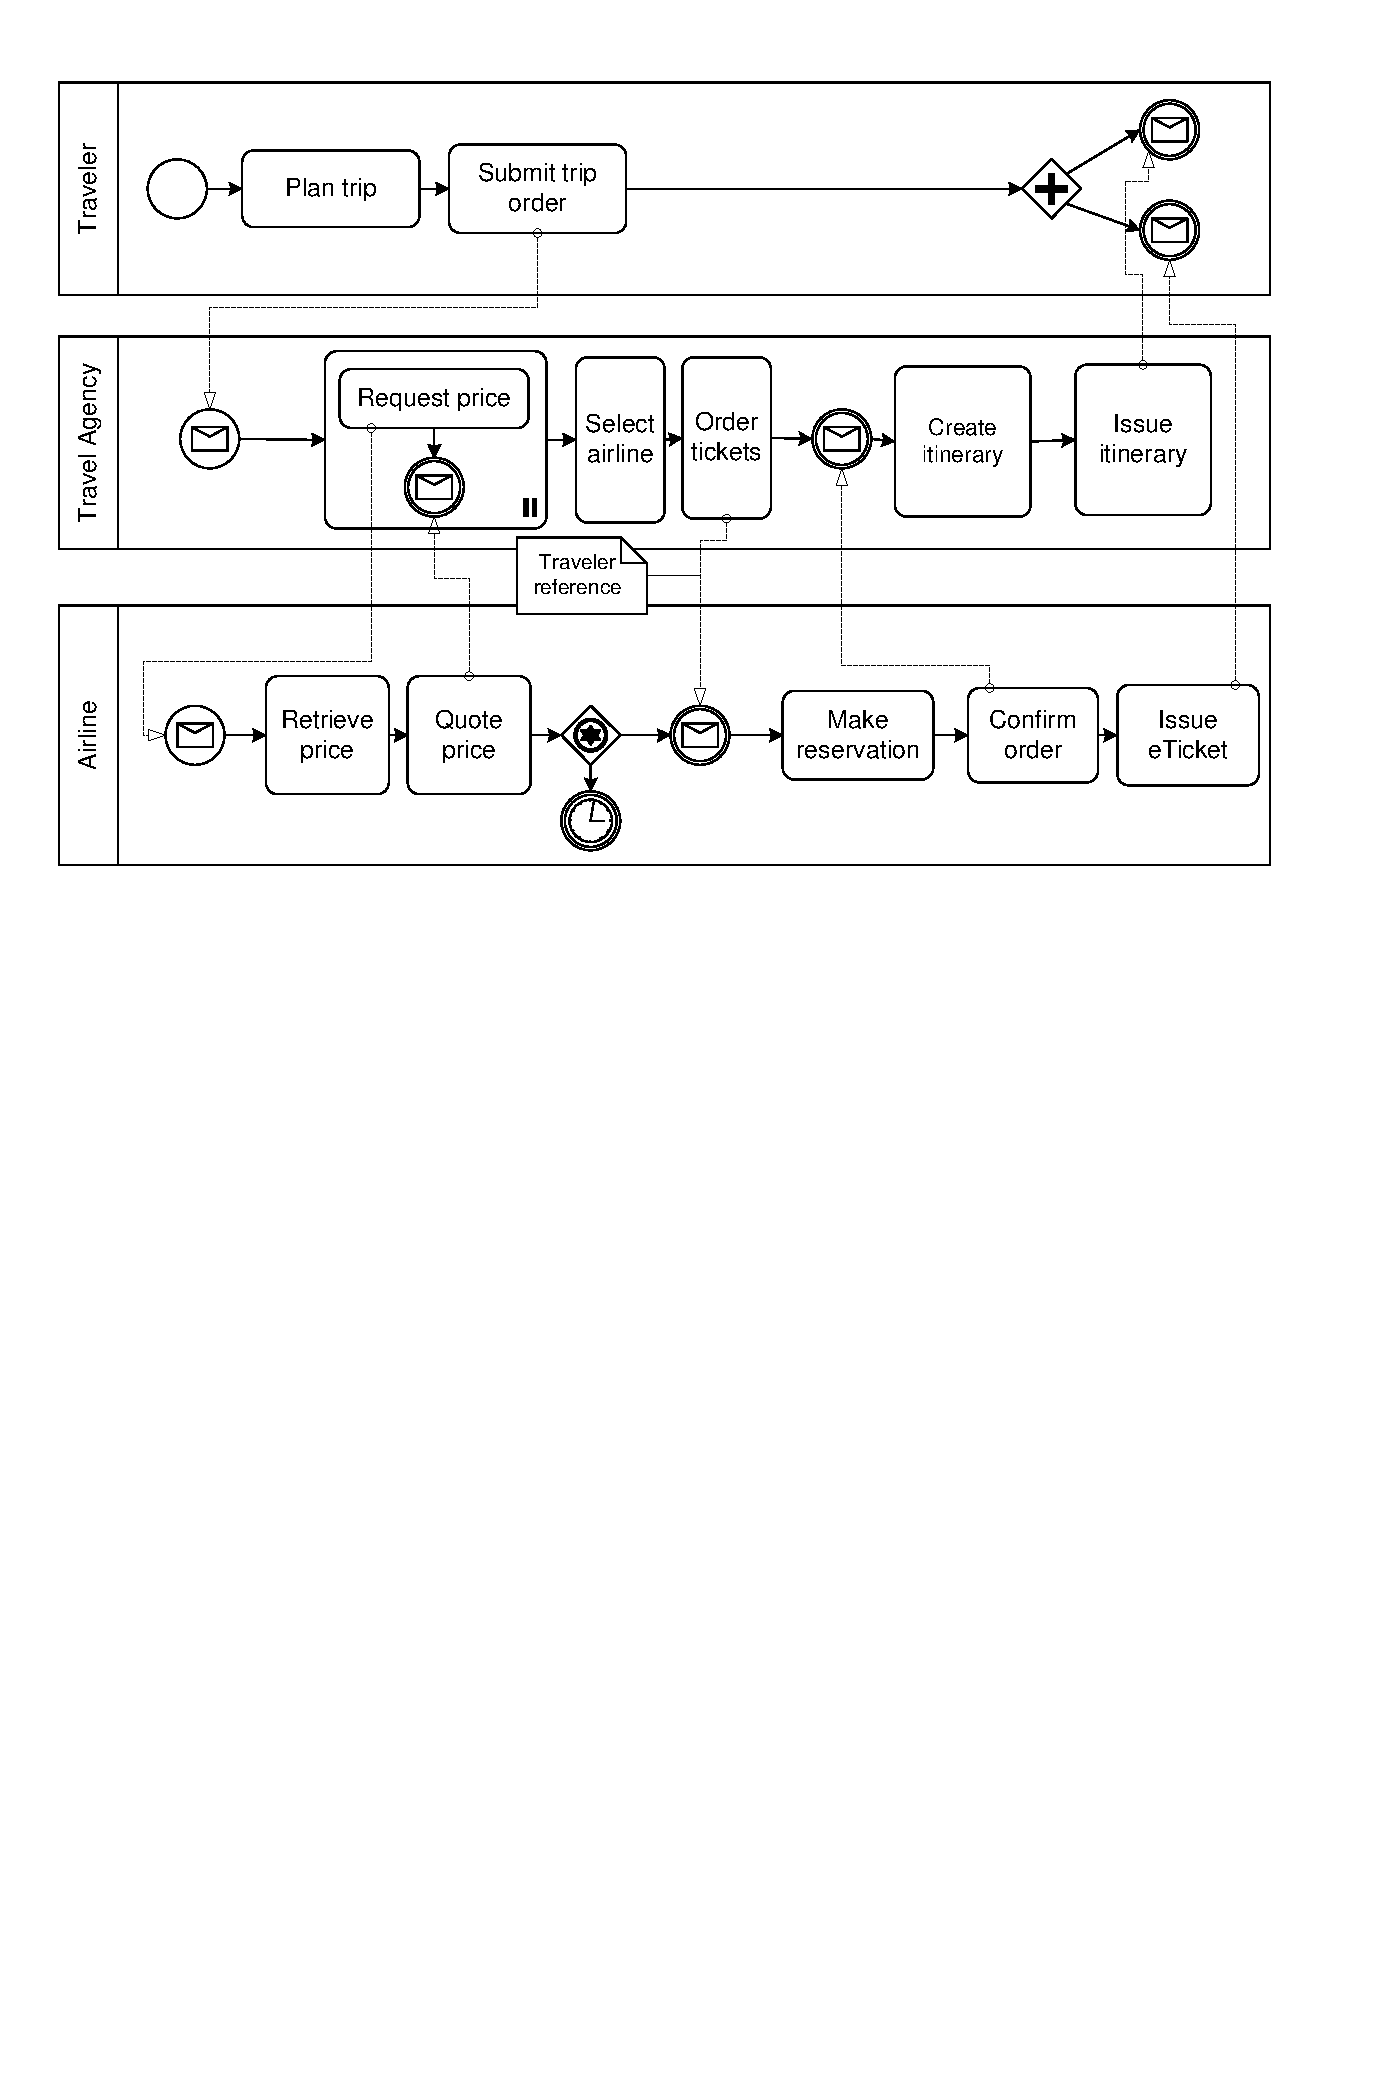
\includegraphics[width=\textwidth]{choreography.pdf}
  \caption{Example Choreography}
  \label{fig:chor1}
\end{figure}

\begin{figure}
  \centering
  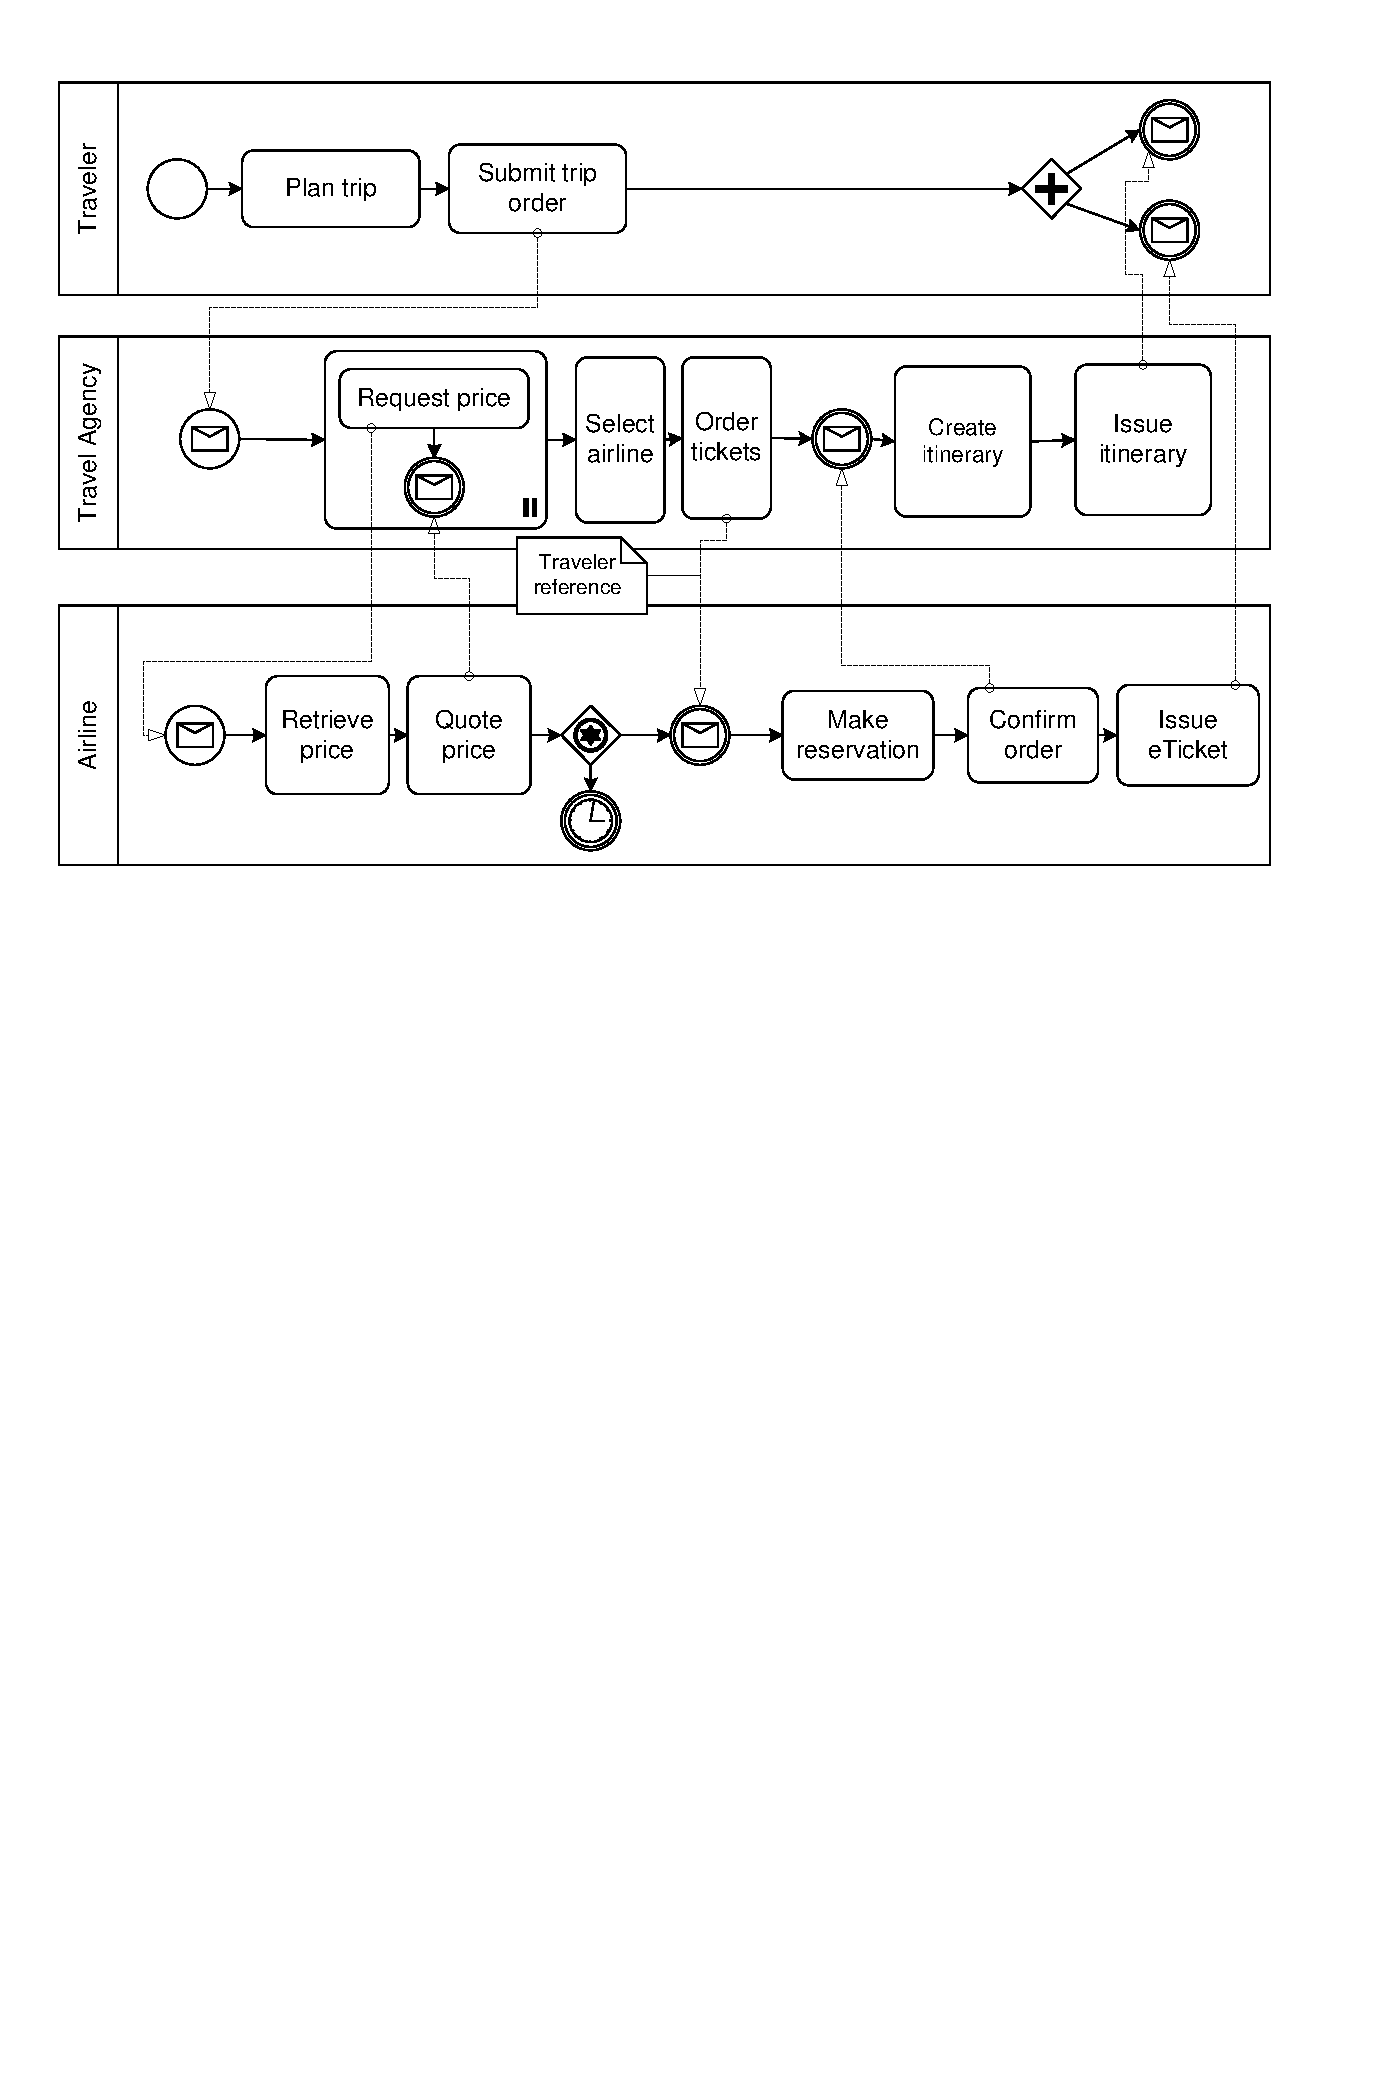
\includegraphics[width=.8\textwidth]{choreography.pdf}
  \caption[Example Choreography]{The example choreography. Now slightly smaller to demonstrate \texttt{\textbackslash textwidth}. And also the use of alternative captions for the list of images. However, the latter is only conditionally recommended, because who reads so much text under a picture? Or is it just a matter of style?}
  \label{fig:chor2}
\end{figure}


\begin{figure}
  \hfill
  \begin{subfigure}{.3\textwidth}
    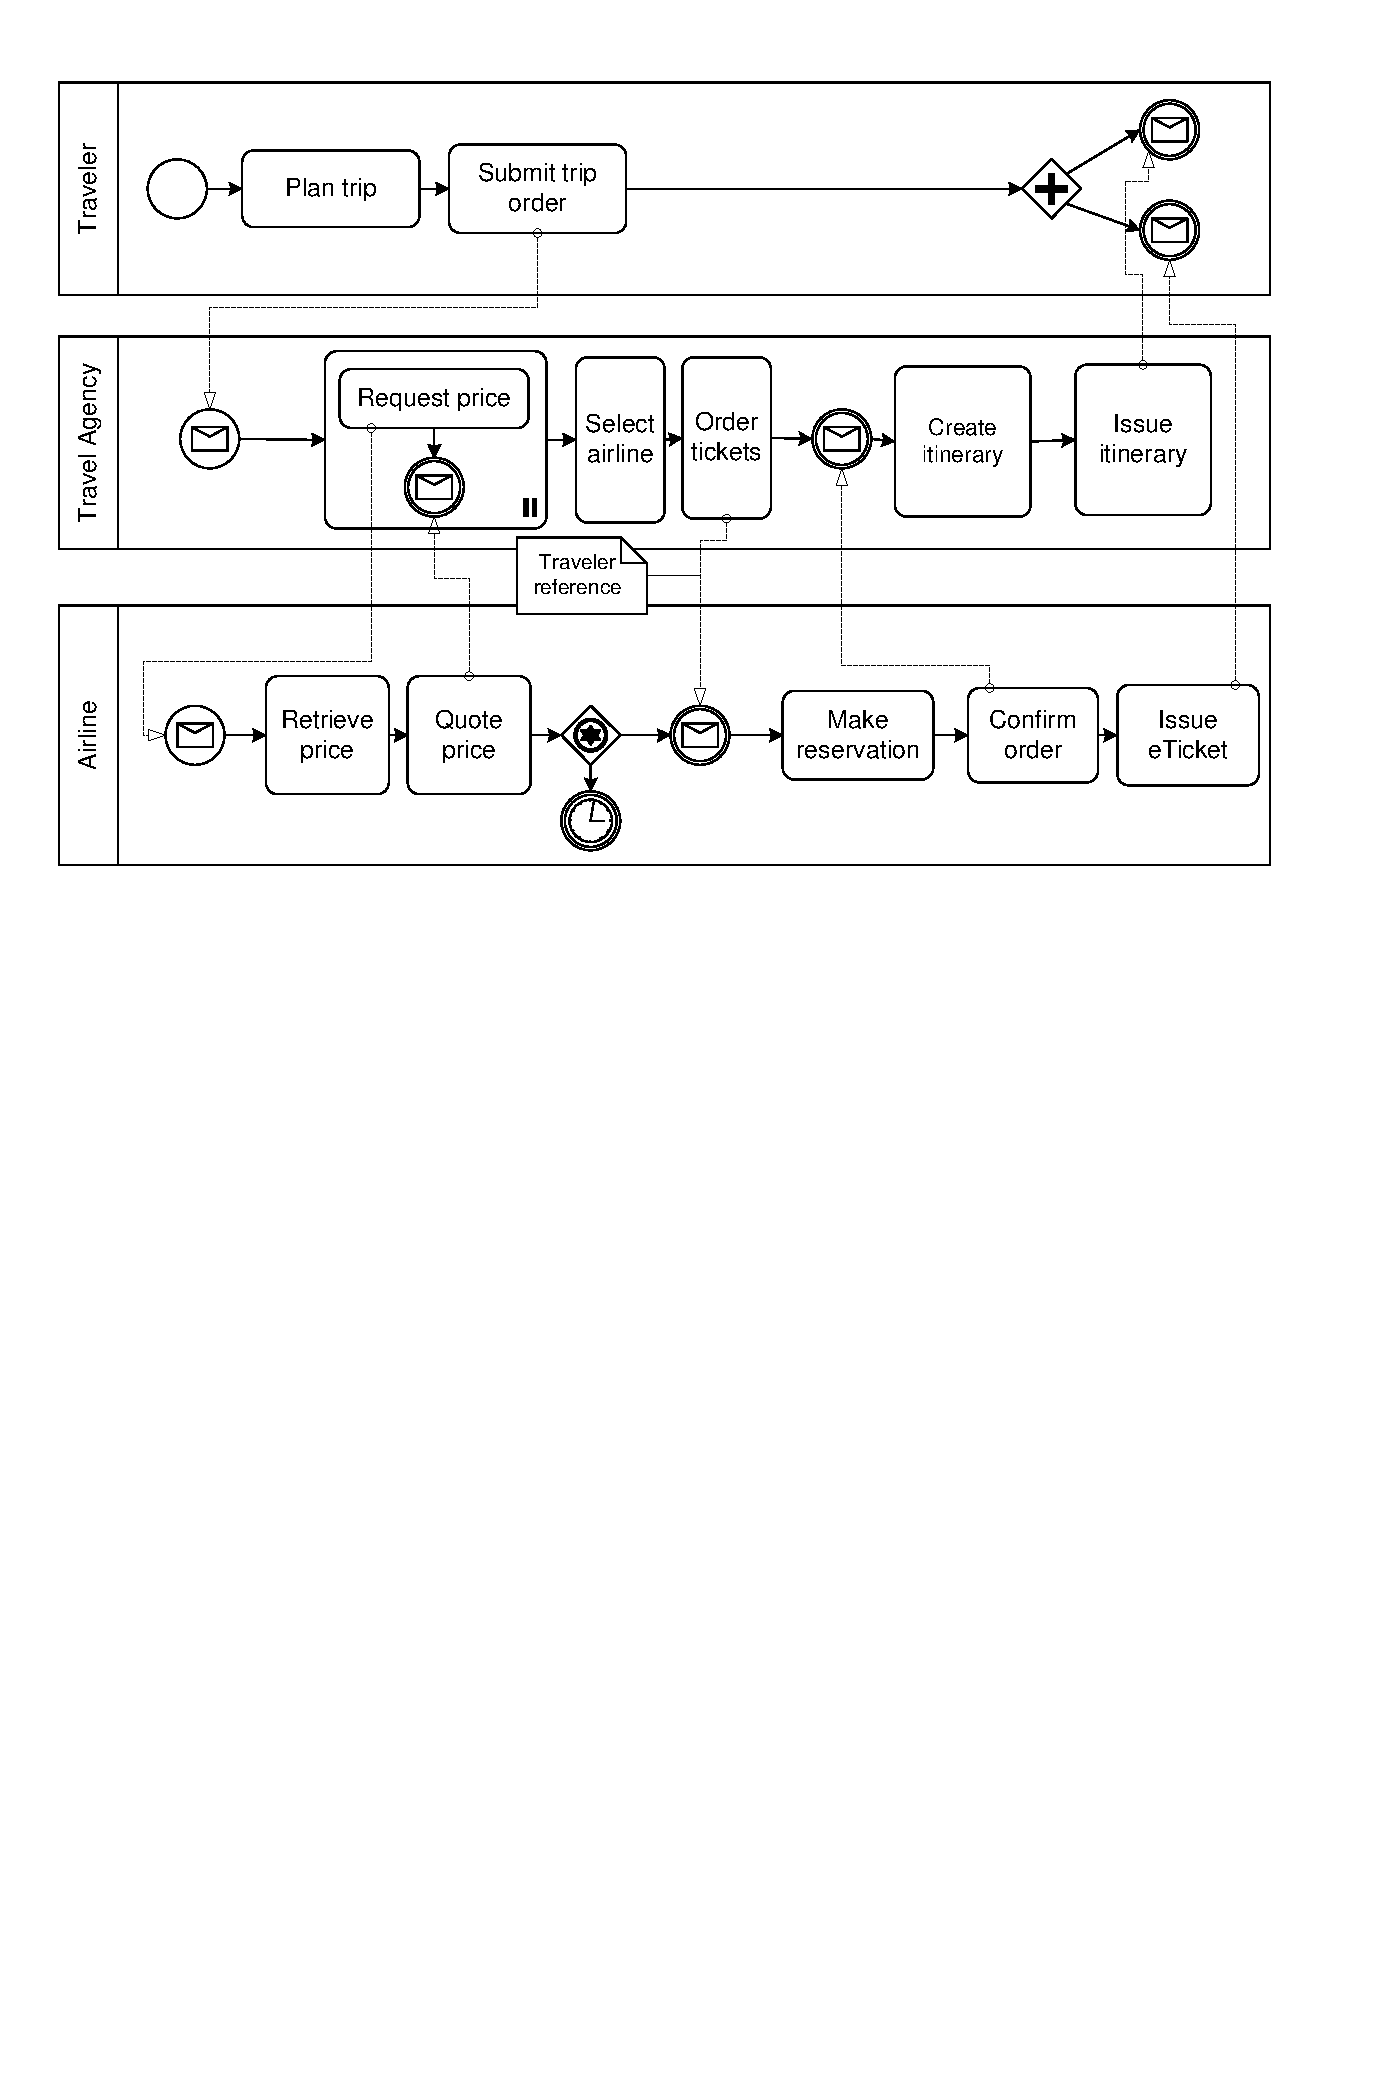
\includegraphics[width=\textwidth]{choreography.pdf}
    \caption{Choreography 1}
    \label{fig:subfigA}
  \end{subfigure}
  \hfill
  \begin{subfigure}{.3\textwidth}
    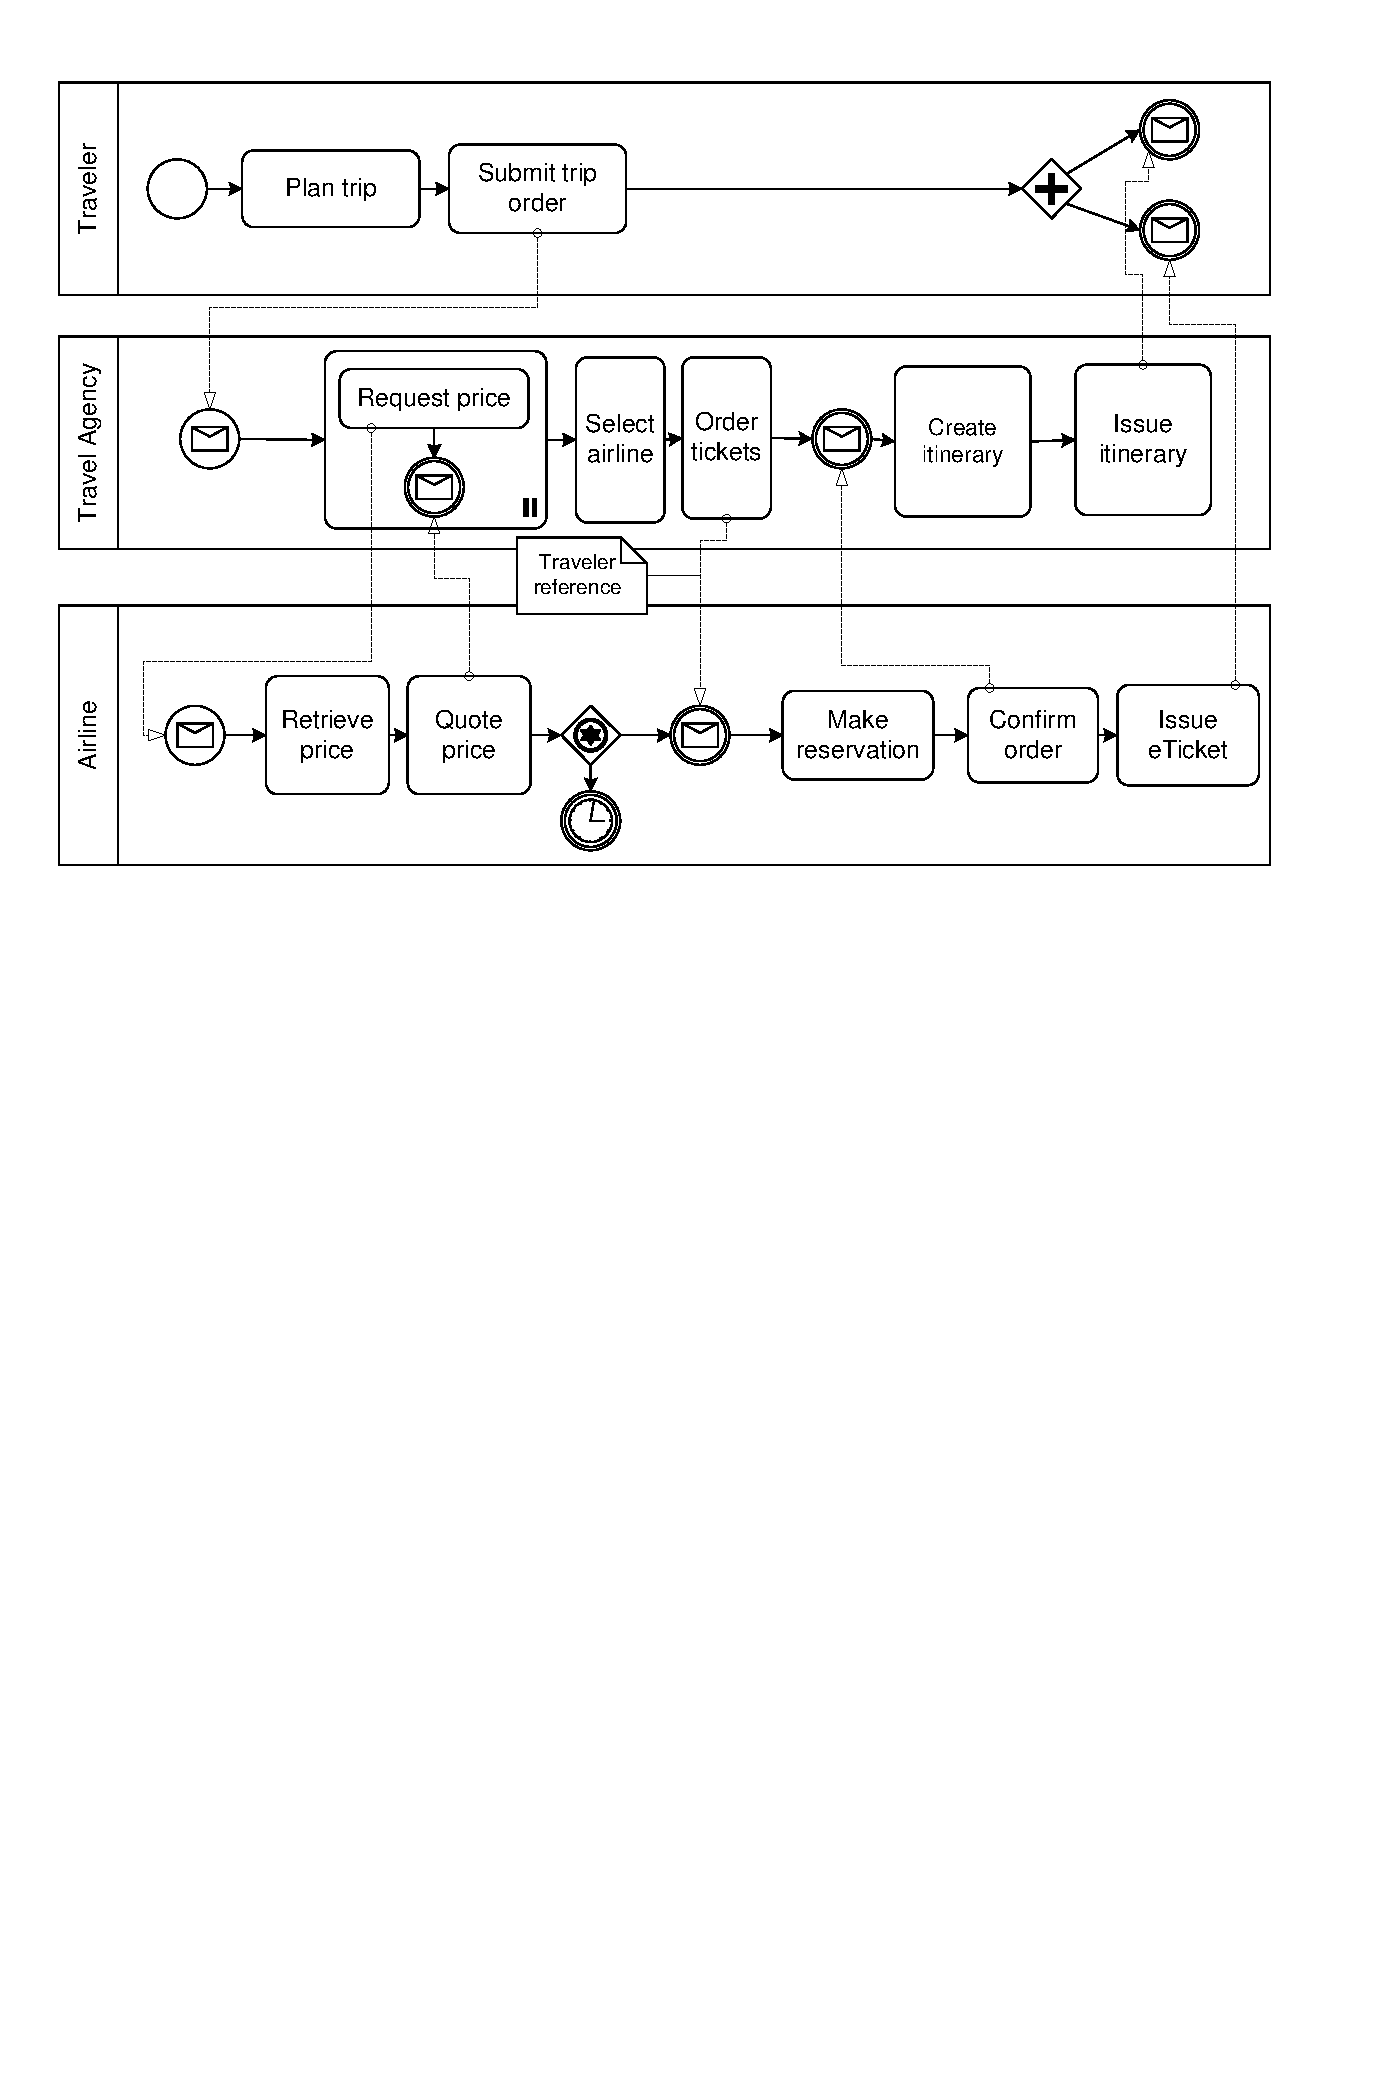
\includegraphics[width=\textwidth]{choreography.pdf}
    \caption{Choreography 2}
    \label{fig:subfigB}
  \end{subfigure}
  \hfill
  \begin{subfigure}{.3\textwidth}
    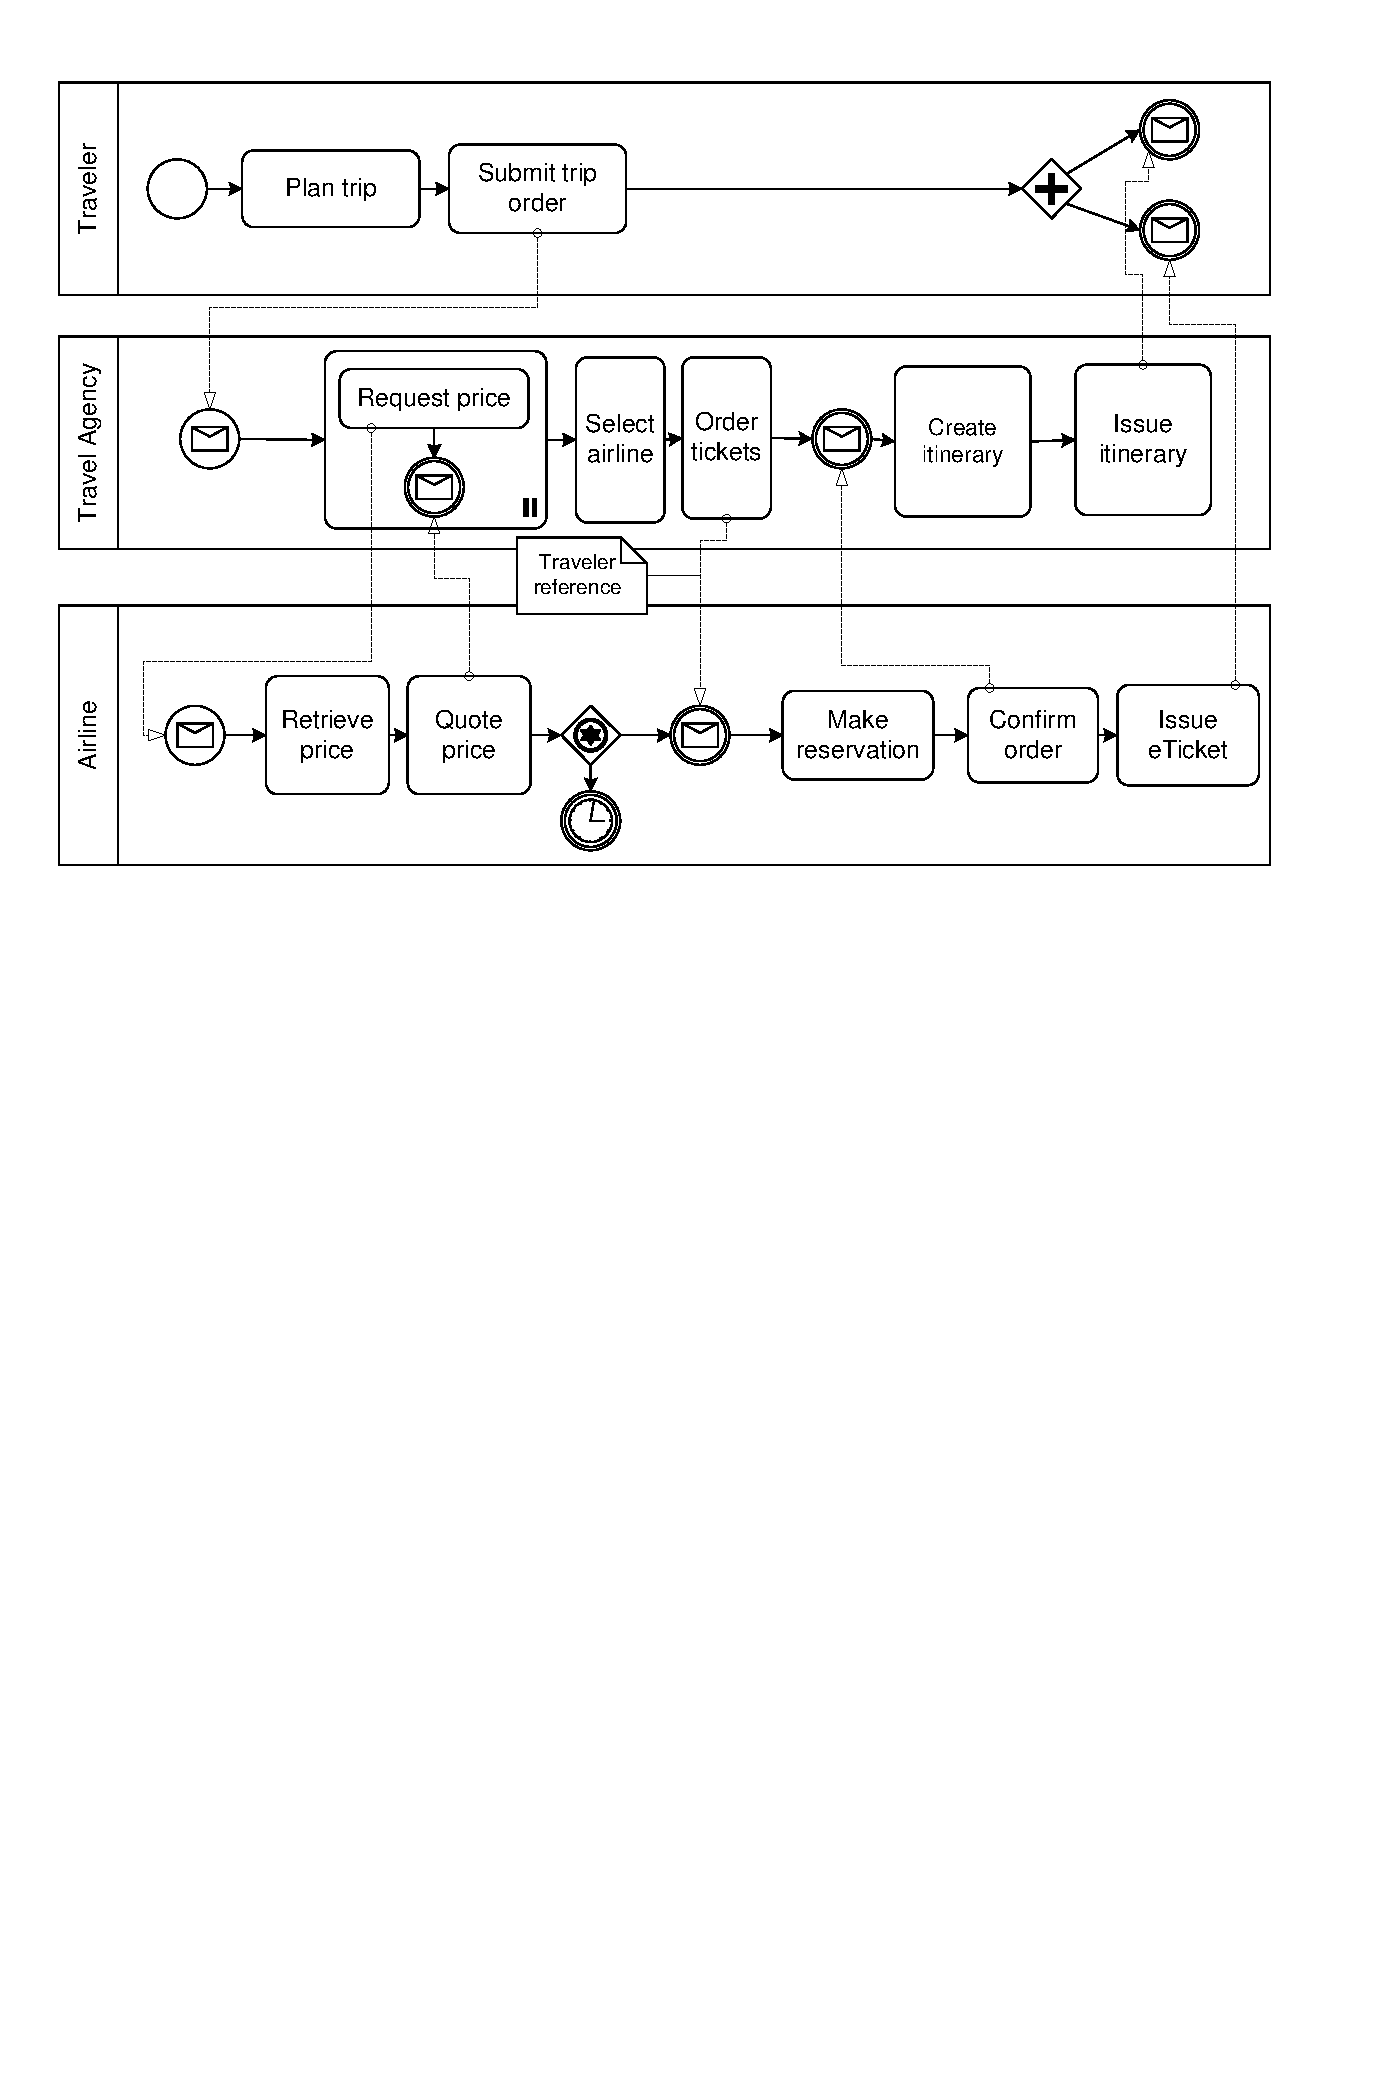
\includegraphics[width=.9\textwidth]{choreography.pdf}
    \caption{Choreography 3}
    \label{fig:subfigC}
  \end{subfigure}
  \caption{Example to place 3 illustrations next to each other. Further, it is possible to reference each separately.}
  \label{fig:subfig_example}
\end{figure}

\Cref{fig:subfig_example} shows the usage of the package subcaption.
It is indeed possible to reference to sub figures: \Cref{fig:subfigA}.

It is possible to convert SVGs to PDF directly during compilation.
This is described in the source code of latex-tipps.tex, but commented out.

\iffalse % <-- Take this away if inkscape is in the path
  The SVG in \cref{fig:directSVG} is directly included, while the text in the SVG in \cref{fig:latexSVG} is set using pdflatex.
  If you want to see the graphics, inkscape must be in PATH and in the text source \texttt{\textbackslash{}iffalse} and \text{\textbackslash{}iftrue} have to be commented out.

  \begin{figure}
    \centering
    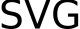
\includegraphics{svgexample.svg}
    \caption{SVG directly included}
    \label{fig:directSVG}
  \end{figure}

  \begin{figure}
    \centering
    \def\svgwidth{.4\textwidth}
    \includesvg{svgexample}
    \caption{Text in SVN set via \LaTeX{}}
    \label{fig:latexSVG}
  \end{figure}
\fi % <-- Take this away if inkscape is in the path



\section{More Illustrations}
\Cref{fig:AnhangsChor,fig:AnhangsChor2} show two choreographies, which should further explain the facts. The second figure is rotated 90 degrees to demonstrate the \texttt{pdflscape} package.

\begin{figure}
  \centering
  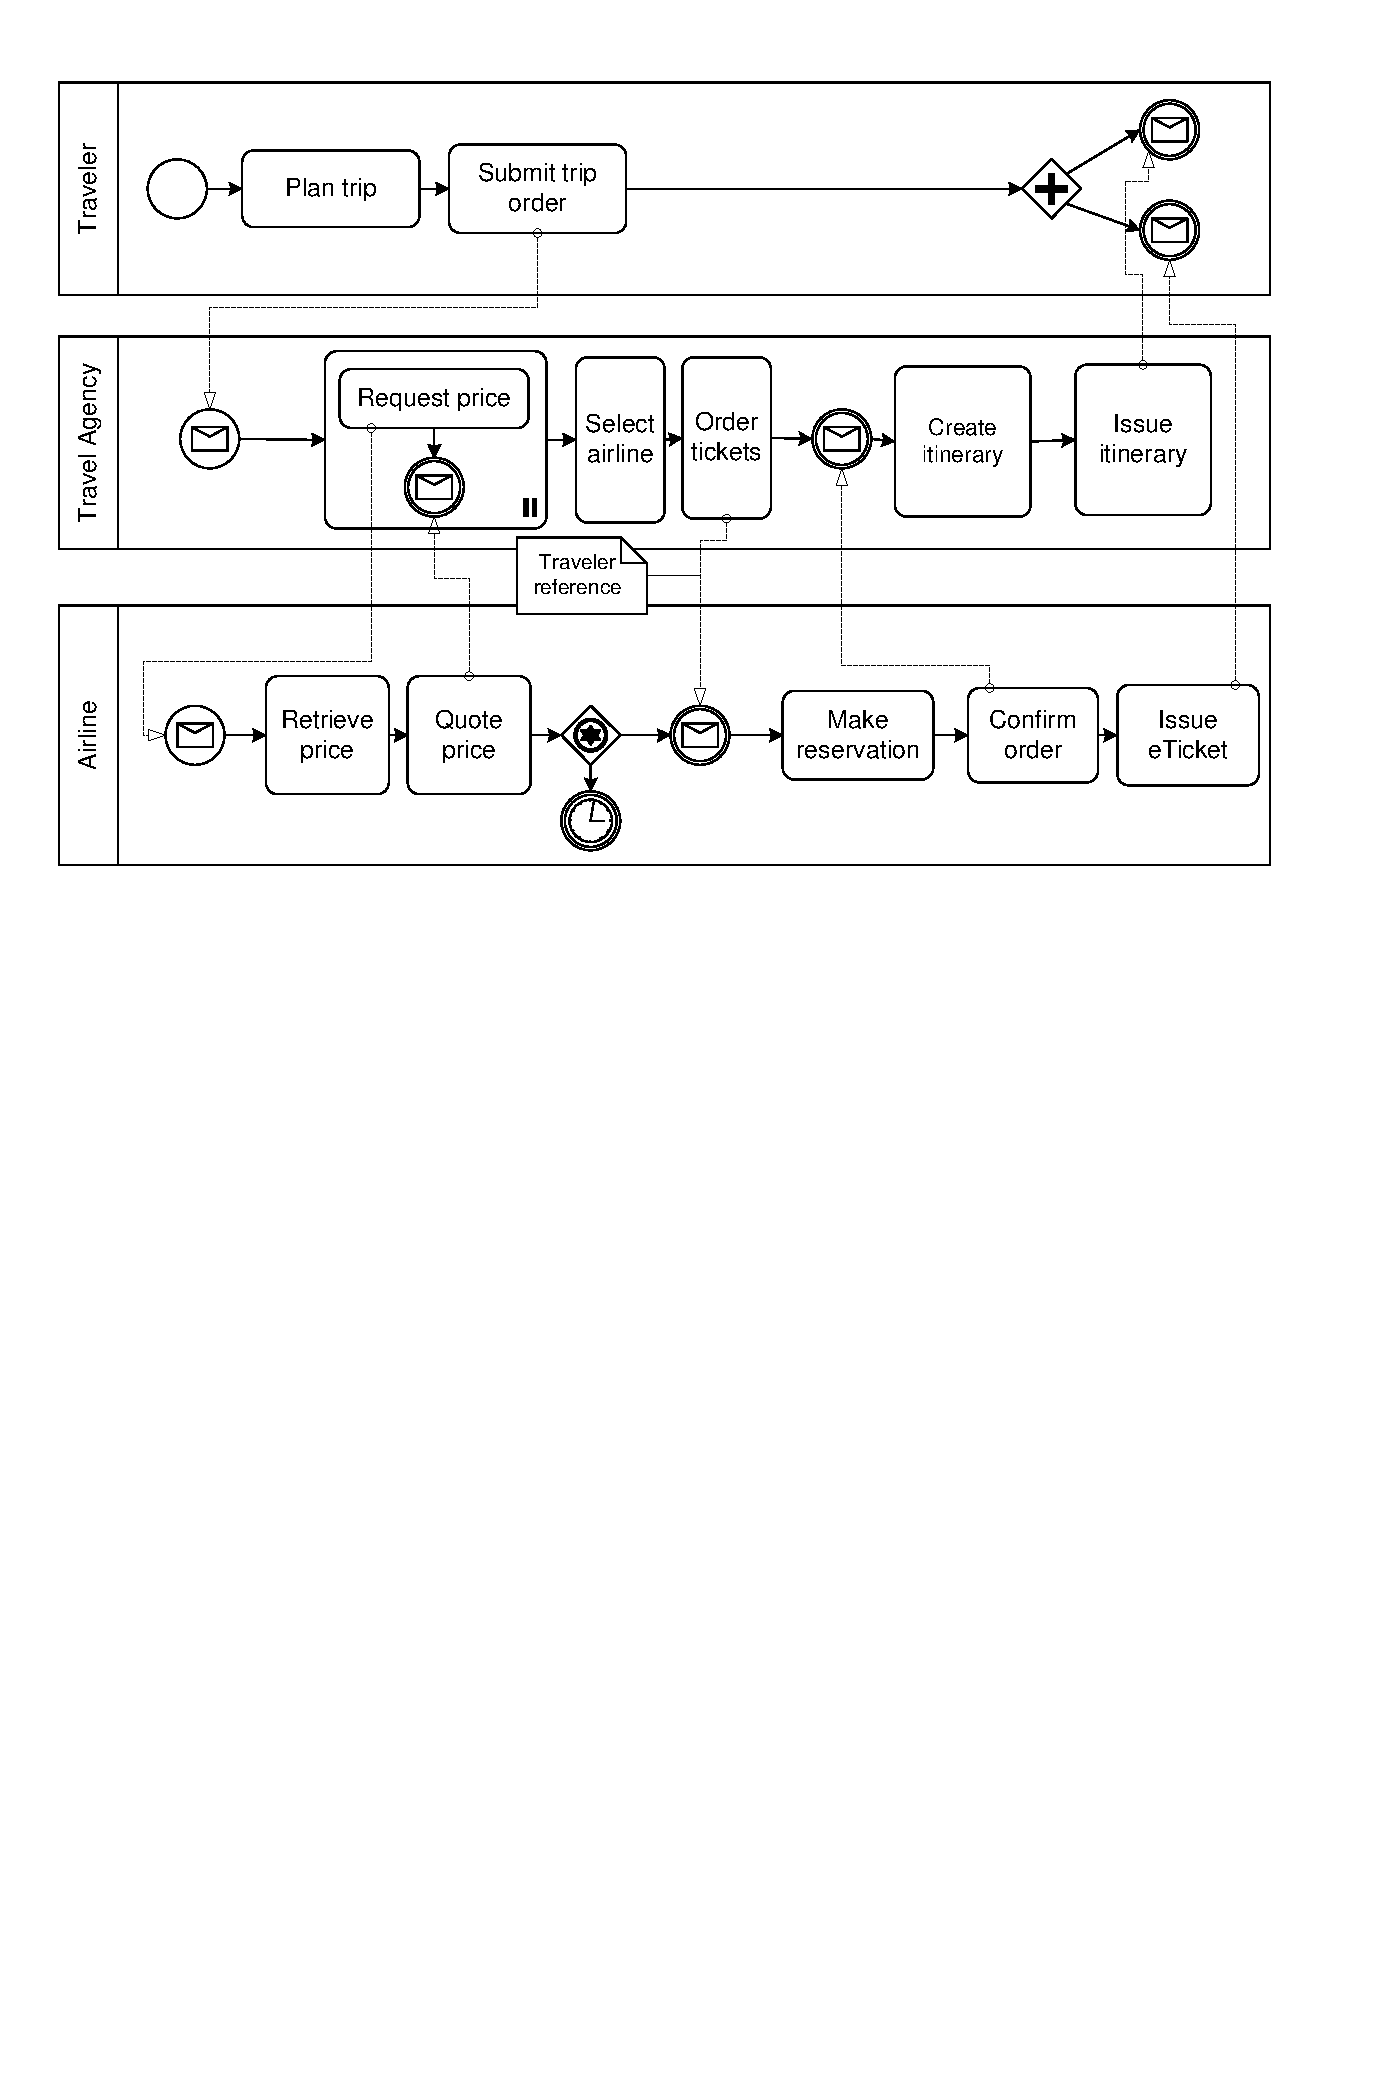
\includegraphics[width=\textwidth]{choreography.pdf}
  \caption{Example Choreography I}
  \label{fig:AnhangsChor}
\end{figure}

\begin{landscape}
  %sidewaysfigure
  \begin{figure}
    \centering
    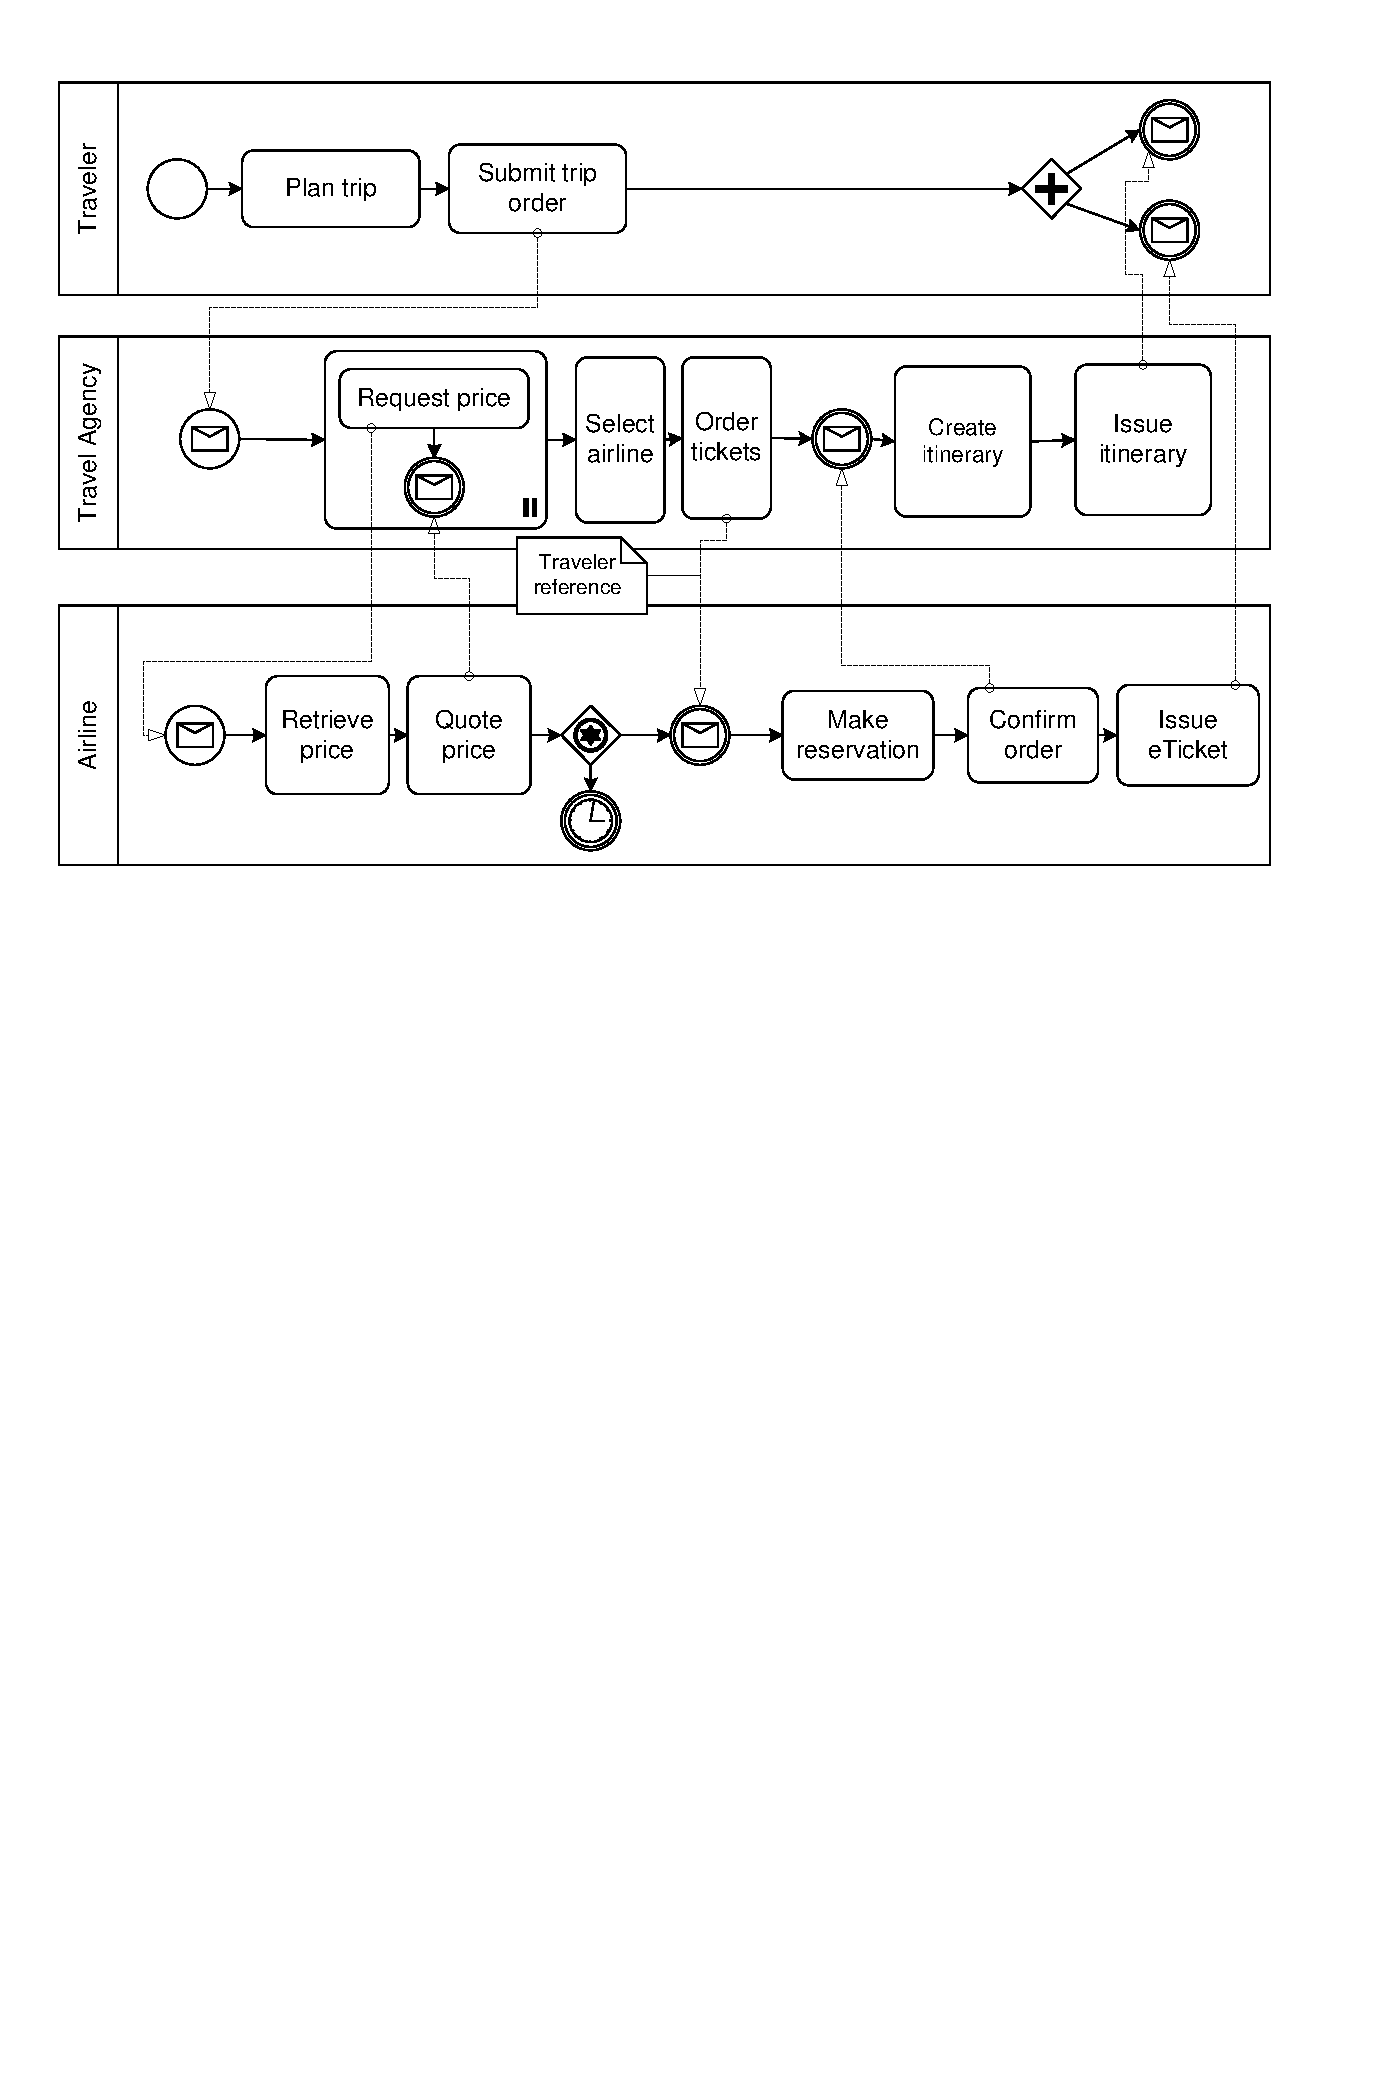
\includegraphics[width=\textwidth]{choreography.pdf}
    \caption{Example Choreography II}
    \label{fig:AnhangsChor2}
  \end{figure}
\end{landscape}


\IfFileExists{pgfplots.sty}{
  %%%%%%%%%%%%%%%%%%%%%%%%%%%%%%%%%%%%%%%%%%%%%%%%%%%%%%%%%%%%%%%%%%%%%%%%%%%%%%
  \section{Plots with pgfplots}
  %%%%%%%%%%%%%%%%%%%%%%%%%%%%%%%%%%%%%%%%%%%%%%%%%%%%%%%%%%%%%%%%%%%%%%%%%%%%%%
  The package pdfplots provides plotting of functions directly in \LaTeX~like with matlab or gnuplot. Some visual examples are available here\footnote{\url{http://texdoc.net/pkg/visualtikz}}.
  \begin{figure}[h]
    \begin{center}
      \begin{tikzpicture}
        \begin{axis}[xlabel=$x$,
            ylabel=$\sin(x)$]
          \addplot {sin(deg(x))};  % Print sine function
        \end{axis}
      \end{tikzpicture}
    \end{center}
    \caption{Plot of $\sin(x)$ direclty inside the figure environment with pgfplots.}
  \end{figure}

  \begin{figure}[h]
    \begin{center}
      \begin{tikzpicture}
        \begin{axis}[xlabel=$x$,
            ylabel=$y$]
          \addplot table [x=a, y=c, col sep=comma] {data/data.csv};  % Read coordinates from csv file and plot them
        \end{axis}
      \end{tikzpicture}
    \end{center}
    \caption{Coordinates $x$ and $y$ read from csv file and plotted pgfplots.}
  \end{figure}

}{}


%%%%%%%%%%%%%%%%%%%%%%%%%%%%%%%%%%%%%%%%%%%%%%%%%%%%%%%%%%%%%%%%%%%%%%%%%%%%%%
\section{Figures with tikz}
%%%%%%%%%%%%%%%%%%%%%%%%%%%%%%%%%%%%%%%%%%%%%%%%%%%%%%%%%%%%%%%%%%%%%%%%%%%%%%
The tikz is a package for creating graphics programmatically. With this package grids or other regular strucutres can be easliy generated.

\begin{figure}[ht]
  \begin{center}
    \begin{tikzpicture}
      \draw(0,0) rectangle (4,4);
      \foreach \x in {0.5,1,1.5,2,2.5,3,3.5}
      \foreach \y in {0.5,1,1.5,2,2.5,3,3.5}
      \draw(\x,\y) circle (1pt);
    \end{tikzpicture}
  \end{center}
  \caption{A regular grid genrated with easily with two for loops.}\label{fig:tikz_example}
\end{figure}


%%%%%%%%%%%%%%%%%%%%%%%%%%%%%%%%%%%%%%%%%%%%%%%%%%%%%%%%%%%%%%%%%%%%%%%%%%%%%%
\section{UML diagrams using tikz-uml}
%%%%%%%%%%%%%%%%%%%%%%%%%%%%%%%%%%%%%%%%%%%%%%%%%%%%%%%%%%%%%%%%%%%%%%%%%%%%%%

\Cref{fig:uml} presents a class diagram typeset using tikz-uml.

\begin{center}
\begin{figure}
\begin{tikzpicture}
\begin{umlpackage}{p}
\begin{umlpackage}{sp1}
\umlclass[template=T]{A}{
  n : uint \\ t : float
}{}
\umlclass[y=-3]{B}{
  d : double
}{
  \umlvirt{setB(b : B) : void} \\ getB() : B}
\end{umlpackage}
\begin{umlpackage}[x=10,y=-6]{sp2}
\umlinterface{C}{
  n : uint \\ s : string
}{}
\end{umlpackage}
\umlclass[x=2,y=-10]{D}{
  n : uint
  }{}
\end{umlpackage}

\umlassoc[geometry=-|-, arg1=tata, mult1=*, pos1=0.3, arg2=toto, mult2=1, pos2=2.9, align2=left]{C}{B}
\umlunicompo[geometry=-|, arg=titi, mult=*, pos=1.7, stereo=vector]{D}{C}
\umlimport[geometry=|-, anchors=90 and 50, name=import]{sp2}{sp1}
\umlaggreg[arg=tutu, mult=1, pos=0.8, angle1=30, angle2=60, loopsize=2cm]{D}{D}
\umlinherit[geometry=-|]{D}{B}
\umlnote[x=2.5,y=-6, width=3cm]{B}{A note with respect to class B}
\umlnote[x=7.5,y=-2]{import-2}{A anotation}
\end{tikzpicture}
\caption{Class diagram generated with tikz-uml. Example adapted from Nicolas Kielbasiewicz.}
\label{fig:uml}
\end{figure}
\end{center}

\section{UML diagrams using PlantUML}

In case \lualatex{} is used and PlantUML is installed, UML diagrams can be defined using PlantUML.

% Only works if "--shell-escape" is activated. Please activate only if you are sure, your compilation settings are correct
%\IfFileExists{plantuml.sty}{\input{latexhints-english-plantuml}}{}

%%%%%%%%%%%%%%%%%%%%%%%%%%%%%%%%%%%%%%%%%%%%%%%%%%%%%%%%%%%%%%%%%%%%%%%%%%%%%%
\section{Tables}
%%%%%%%%%%%%%%%%%%%%%%%%%%%%%%%%%%%%%%%%%%%%%%%%%%%%%%%%%%%%%%%%%%%%%%%%%%%%%%
\cref{tab:Ergebnisse} shows results and \cref{tab:Results} shows how numerical data can be represented in a table.
\begin{table}
  \centering
  \begin{tabular}{ccc}
    \toprule
    \multicolumn{2}{c}{\textbf{summed}} & \textbf{Title}                                                          \\ \midrule
    Table                                      & as                                                           & in      \\
    \url{tabsatz.pdf}                            & recommended                                                     & gesetzt \\

    \multirow{2}{*}{Example}                    & \multicolumn{2}{c}{a nice example}                                \\
                                                 & \multicolumn{2}{c}{for using \qq{multirow}}           \\
    \bottomrule
  \end{tabular}
  \caption[Example Table]{Exampe Table -- see \url{http://www.ctan.org/tex-archive/info/german/tabsatz/}}
  \label{tab:Ergebnisse}
\end{table}

\begin{table}
  \centering
  \begin{tabular}{l *{8}{d{3.2}}}
    \toprule

                         & \multicolumn{2}{c}{\textbf{Parameter 1}} & \multicolumn{2}{c}{\textbf{Parameter 2}} & \multicolumn{2}{c}{\textbf{Parameter 3}} & \multicolumn{2}{c}{\textbf{Parameter 4}}                                                                                                                                       \\
    \cmidrule(r){2-3}\cmidrule(lr){4-5}\cmidrule(lr){6-7}\cmidrule(l){8-9}

    \textbf{Bedingungen} & \multicolumn{1}{c}{\textbf{M}}           & \multicolumn{1}{c}{\textbf{SD}}          & \multicolumn{1}{c}{\textbf{M}}           & \multicolumn{1}{c}{\textbf{SD}}          & \multicolumn{1}{c}{\textbf{M}} & \multicolumn{1}{c}{\textbf{SD}} & \multicolumn{1}{c}{\textbf{M}} & \multicolumn{1}{c}{\textbf{SD}} \\
    \midrule

    W                    & 1.1                                      & 5.55                                     & 6.66                                     & .01                                      &                                &                                 &                                &                                 \\
    X                    & 22.22                                    & 0.0                                      & 77.5                                     & .1                                       &                                &                                 &                                &                                 \\
    Y                    & 333.3                                    & .1                                       & 11.11                                    & .05                                      &                                &                                 &                                &                                 \\
    Z                    & 4444.44                                  & 77.77                                    & 14.06                                    & .3                                       &                                &                                 &                                &                                 \\
    \bottomrule
  \end{tabular}

  \caption{Example table for 4 constraints (W-Z), each having 4 parameters with (M und SD). Note: use always the same number of decimal places.}
  \label{tab:Werte}
\end{table}

\IfFileExists{pgfplotstable.sty}{

\subsection{Tables with pgfplots}
With the pgfplotstable package tables can be directly generated from a csv file.

\begin{table}[h]
\centering
\pgfplotstabletypeset[
col sep = comma,
every head row/.style={before row=\toprule,after row=\midrule},
every last row/.style={after row=\bottomrule},
display columns/0/.style={string type,column name={}}
]
{data/data.csv}
\caption{Table direclty generated from the values of a csf file.}
\end{table}
}{}


\section{Tables spanning multiple pages}


\begin{longtable}{|l|l|l|}
\caption{A sample long table.} \label{tab:long} \\

\hline \multicolumn{1}{|c|}{\textbf{First column}} & \multicolumn{1}{c|}{\textbf{Second column}} & \multicolumn{1}{c|}{\textbf{Third column}} \\ \hline
\endfirsthead

\multicolumn{3}{c}%
{{\bfseries \tablename\ \thetable{} -- continued from previous page}} \\
\hline \multicolumn{1}{|c|}{\textbf{First column}} & \multicolumn{1}{c|}{\textbf{Second column}} & \multicolumn{1}{c|}{\textbf{Third column}} \\ \hline
\endhead

\hline \multicolumn{3}{|r|}{{Continued on next page}} \\ \hline
\endfoot

\hline \hline
\endlastfoot

A & BC & D \\
A & BC & D \\
A & BC & D \\
A & BC & D \\
A & BC & D \\
A & BC & D \\
A & BC & D \\
A & BC & D \\
A & BC & D \\
A & BC & D \\
A & BC & D \\
A & BC & D \\
A & BC & D \\
A & BC & D \\
A & BC & D \\
A & BC & D \\
A & BC & D \\
A & BC & D \\
A & BC & D \\
A & BC & D \\
A & BC & D \\
A & BC & D \\
A & BC & D \\
A & BC & D \\
A & BC & D \\
A & BC & D \\
A & BC & D \\
A & BC & D \\
A & BC & D \\
A & BC & D \\
A & BC & D \\
A & BC & D \\
A & BC & D \\
A & BC & D \\
A & BC & D \\
A & BC & D \\
A & BC & D \\
A & BC & D \\
A & BC & D \\
A & BC & D \\
A & BC & D \\
A & BC & D \\
A & BC & D \\
A & BC & D \\
A & BC & D \\
A & BC & D \\
A & BC & D \\
A & BC & D \\
A & BC & D \\
A & BC & D \\
A & BC & D \\
A & BC & D \\
A & BC & D \\
A & BC & D \\
A & BC & D \\
A & BC & D \\
A & BC & D \\
A & BC & D \\
A & BC & D \\
A & BC & D \\
A & BC & D \\
A & BC & D \\
A & BC & D \\
A & BC & D \\
A & BC & D \\
A & BC & D \\
A & BC & D \\
A & BC & D \\
A & BC & D \\
A & BC & D \\
A & BC & D \\
A & BC & D \\
A & BC & D \\
A & BC & D \\
A & BC & D \\
A & BC & D \\
A & BC & D \\
A & BC & D \\
A & BC & D \\
A & BC & D \\
\end{longtable}


%%%%%%%%%%%%%%%%%%%%%%%%%%%%%%%%%%%%%%%%%%%%%%%%%%%%%%%%%%%%%%%%%%%%%%%%%%%%%%
\section{Abbreviations}
%%%%%%%%%%%%%%%%%%%%%%%%%%%%%%%%%%%%%%%%%%%%%%%%%%%%%%%%%%%%%%%%%%%%%%%%%%%%%%
At the first pass the \gls{fr} was 5.
At the second pass was \gls{fr} 3.
The plural form can be seen here: \glspl{er}.
To demonstrate what the list of abbreviations looks like for longer description texts, \glspl{rdbms} must be mentioned here.

With \verb+\gls{...}+ you can enter abbreviations, the first time you call it, the long form is used.
When reusing \verb+\gls{..}+ the short form is automatically displayed.
The abbreviation is also automatically inserted in the abbreviation list.
With \verb+\glspl{...}+ the plural form is used.
If you want the short form to appear directly at the first use, you can use \verb+\glsunset{..}+ to mark an abbreviation as already used.
The opposite is achieved with \verb+\glsreset{..}+.

Abbreviations are defined in \textit{content\\ausarbeitung.tex} by means of \verb+\newacronym{...}{...}{...}+.

More information at: \url{http://tug.ctan.org/macros/latex/contrib/glossaries/glossariesbegin.pdf}
%%%%%%%%%%%%%%%%%%%%%%%%%%%%%%%%%%%%%%%%%%%%%%%%%%%%%%%%%%%%%%%%%%%%%%%%%%%%%%
\section{References}
%%%%%%%%%%%%%%%%%%%%%%%%%%%%%%%%%%%%%%%%%%%%%%%%%%%%%%%%%%%%%%%%%%%%%%%%%%%%%%
For distant sections \qq{varioref} is recommended:
\qq{See \vref{sec:mf}}.
The command \texttt{\textbackslash{}vref} works similar to \texttt{\textbackslash{}cref} the difference beeing that a reference to the page is additionally added.
\texttt{vref}: \qq{\vref{sec:firstsectioninlatexhints}}, \texttt{cref}: \qq{\cref{sec:firstsectioninlatexhints}}, \texttt{ref}: \qq{\ref{sec:firstsectioninlatexhints}}.

If \qq{varioref} causes difficulties, then \qq{cref} can be used instead.
This also creates the word \qq{section} automatically: \cref{sec:mf}.
This is also possible for illustrations etc.
In English please use \verb1\Cref{...}1 (with large \qq{C} at the beginning).

%With MiKTeX installation from 2012-01-16 no longer necessary.
%If a section becomes longer than one page and you want to refer to a specific place in the section with \texttt{\textbackslash{}vref}, then you should use \texttt{\textbackslash{}phantomsection} then using \texttt{vref} will also display the correct page number.

%%The link location will be placed on the line below.
%%Tipp von http://en.wikibooks.org/wiki/LaTeX/Labels_and_Cross-referencing#The_hyperref_package_and_.5Cphantomsection
%\phantomsection
%\label{alabel}
%View the example for \texttt{\textbackslash{}phantomsection} in the \LaTeX{} source code.

%Here is the example: See Section \vref{hack1} and Section \vref{hack2}.
%%%%%%%%%%%%%%%%%%%%%%%%%%%%%%%%%%%%%%%%%%%%%%%%%%%%%%%%%%%%%%%%%%%%%%%%%%%%%%
\section{Definitions}
%%%%%%%%%%%%%%%%%%%%%%%%%%%%%%%%%%%%%%%%%%%%%%%%%%%%%%%%%%%%%%%%%%%%%%%%%%%%%%
\begin{definition}[Title]
  \label{def:def1}
  Definition Text
\end{definition}

\Cref{def:def1} shows \ldots

%%%%%%%%%%%%%%%%%%%%%%%%%%%%%%%%%%%%%%%%%%%%%%%%%%%%%%%%%%%%%%%%%%%%%%%%%%%%%%
\section{Footnotes}
%%%%%%%%%%%%%%%%%%%%%%%%%%%%%%%%%%%%%%%%%%%%%%%%%%%%%%%%%%%%%%%%%%%%%%%%%%%%%%
Footnotes are provided by the command \verb+\footnote{...}+\footnote{\label{fussnote}Example footnote.}. Citing footnotes is possible by provinding a label\verb+\footnote{\label{...}...}+ and cite the footnote with \verb+\cref{...}+ in the text\cref{fussnote}.
%%%%%%%%%%%%%%%%%%%%%%%%%%%%%%%%%%%%%%%%%%%%%%%%%%%%%%%%%%%%%%%%%%%%%%%%%%%%%%

%%%%%%%%%%%%%%%%%%%%%%%%%%%%%%%%%%%%%%%%%%%%%%%%%%%%%%%%%%%%%%%%%%%%%%%%%%%%%%
\section{Various Things}
%%%%%%%%%%%%%%%%%%%%%%%%%%%%%%%%%%%%%%%%%%%%%%%%%%%%%%%%%%%%%%%%%%%%%%%%%%%%%%
\label{sec:diff}
\ifdeutsch
  Numbers (123\,654\,789) are nicely set.
  Either in a line or as non-lining figure.
  The latter is reached by parameter \texttt{osf} at package \texttt{libertine} or.\ \texttt{mathpazo} in \text{fonts.tex}.
\fi

\begin{filecontents*}{\democodefile}
\begin{compactenum}[I.]
  \item You can also keep the numbering compact thanks to paralist
  \item and switch to a different numbering
\end{compactenum}
\end{filecontents*}
\PrintDemo{style=parallel}

The words \qq{workflow} and \qq{dwarflike} can be copied from the PDF and pasted to a text file.

\begin{filecontents*}{\democodefile}
In case \LuaLaTeX{} is used as compiler, there is no ligature at \qq{f\/l} in the word \qq{dwarflike} (in contrast to \qq{fl} at \qq{workflow}).
In other words: \qq{dwarflike} and \qq{dwarf\/like} look the same in the PDF.
In case they do not, there is an issue with Lua\LaTeX{} and the selnolig package.
\end{filecontents*}
\PrintDemo{style=parallel}
% Meta comment: The precise form of the optimal ligation suppression command may vary depending on the character pairs involved - see https://tex.stackexchange.com/q/28437/9075


%%%%%%%%%%%%%%%%%%%%%%%%%%%%%%%%%%%%%%%%%%%%%%%%%%%%%%%%%%%%%%%%%%%%%%%%%%%%%%
\section{Closing remarks}
%%%%%%%%%%%%%%%%%%%%%%%%%%%%%%%%%%%%%%%%%%%%%%%%%%%%%%%%%%%%%%%%%%%%%%%%%%%%%%
Please feel free to provide enhancements for this template and create a new ticket on GitHub (\url{https://github.com/latextemplates/uni-stuttgart-computer-science-template/issues}).


\pagestyle{empty}
\renewcommand*{\chapterpagestyle}{empty}
\Versicherung

\end{document}
